%% Version 5.0, 2 January 2020
%
%%%%%%%%%%%%%%%%%%%%%%%%%%%%%%%%%%%%%%%%%%%%%%%%%%%%%%%%%%%%%%%%%%%%%%
% amspaperV5.tex --  LaTeX-based template for submissions to American 
% Meteorological Society journals
%
%
%%%%%%%%%%%%%%%%%%%%%%%%%%%%%%%%%%%%%%%%%%%%%%%%%%%%%%%%%%%%%%%%%%%%%
% PREAMBLE
%%%%%%%%%%%%%%%%%%%%%%%%%%%%%%%%%%%%%%%%%%%%%%%%%%%%%%%%%%%%%%%%%%%%%

%% Start with one of the following:
% DOUBLE-SPACED VERSION FOR SUBMISSION TO THE AMS
\documentclass{ametsocV5}

% TWO-COLUMN JOURNAL PAGE LAYOUT---FOR AUTHOR USE ONLY
% \documentclass[twocol]{ametsocV5}


% Enter packages here. If too many math alphabets are used,
% remove unnecessary packages or define hmmax and bmmax as necessary.

%\newcommand{\hmmax}{0}
%\newcommand{\bmmax}{0}
\usepackage{amsmath,amsfonts,amssymb,bm}
\usepackage{mathptmx}%{times}
\usepackage{newtxtext}
\usepackage{newtxmath}


%%% To be entered by author:

\newcommand{\appbEqnSoln}{Appendix~A}
\newcommand{\appFGEqnSoln}{Appendix~B}
\newcommand{\appnumSoln}{Appendix~C}
\newif\ifshowfootnotes
\showfootnotestrue   % development: show footnotes
% \showfootnotesfalse % production: hide footnotes

\newcommand{\myfootnote}[1]{%
  \ifshowfootnotes
    \footnote{#1}%
  \fi
}

\newcommand{\Claude}[1]{{\color{red}{#1}}}

% Tracked changes. Edits made in the repository Manuscript/ folder are marked
% with \added, \deleted, and \replaced (author CL): insertions in blue,
% deletions struck through, and a list of changes after the title. To accept
% every change, load the package as \usepackage[final]{changes}.
\usepackage{changes}
\definechangesauthor[name={Claude}, color=blue]{CL}
% Review corrections of 2026-10-26, for checking.
\definechangesauthor[name={Claude review}, color=magenta]{CR}
% For struck-out mathematics in CR changes; remove with them.
\usepackage{cancel}
\newcommand{\CRnew}[1]{{\color{magenta}#1}}
\newcommand{\CRold}[1]{{\color{magenta}\cancel{#1}}}

%% May use \\ to break lines in title:

\title{On Robust Diagnostic Planetary Geostrophy}

%%% Enter authors' names, as you see in this example:
%%% Use \correspondingauthor{} and \thanks{Current Affiliation:...}
%%% immediately following the appropriate author.
%%%
%%% Note that the \correspondingauthor{} command is NECESSARY.
%%% The \thanks{} commands are OPTIONAL.

    \authors{Thomas W. N. Haine\correspondingauthor{Thomas Haine, Thomas.Haine@jhu.edu}}

     \affiliation{Earth \& Planetary Sciences, Johns Hopkins University, Baltimore, MD, }

%%%%%%%%%%%%%%%%%%%%%%%%%%%%%%%%%%%%%%%%%%%%%%%%%%%%%%%%%%%%%%%%%%%%%
% ABSTRACT
%
% Enter your Abstract here

\abstract{Planetary geostrophy (PG) with a prescribed density field, the robust-diagnostic approximation, determines the steady large-scale ocean circulation from the surface stress, the surface buoyancy, and a restoring buoyancy field. We solve the linear robust-diagnostic PG equations exactly, with vertical friction and diffusion, over arbitrary bathymetry and Coriolis parameter. Closed-form Green's functions give the buoyancy and horizontal velocity in each water column, resolving the surface and bottom Ekman layers even where they overlap. The surface pressure then satisfies one two-dimensional advection--diffusion equation with exact column-integral coefficients, which is solved with finite elements and no normal flow at the coast. The solution is verified by mesh convergence, by closure of the depth-integrated momentum and vorticity balances, and against a numerical primitive-equation model to 1--2\%, at 25 to 150 times lower cost. 
It recovers the Sverdrup--Stommel gyre, $\beta$ plumes in open water and beside a coast, and topographic steering, and quantifies the corrections to these classical results.
The Ekman drag varies as $f^{1/2}$ for Coriolis parameter $f$, and the bottom Ekman layer of depth $\delta_E$ acts as a displacement thickness so that the flow follows $f/(H - \delta_E/2)$ contours, where $H$ is the water depth.
Steering by these contours fails where $H \lessapprox 2 \delta_E$. 
In a double basin joined by a strait, the integral constraint of N\o st and Isachsen on closed $f/H$ contours reproduces the bottom velocity to 3\% with the derived bottom stress, \added[id=CL]{but errs by more than 100\% with a calibrated isotropic drag.}
One adjoint sensitivity solve maps the forcing that sets the strait transport. 
}

\begin{document}


%% Necessary!
\maketitle
\listofchanges[style=summary]

%%%%%%%%%%%%%%%%%%%%%%%%%%%%%%%%%%%%%%%%%%%%%%%%%%%%%%%%%%%%%%%%%%%%%
% SIGNIFICANCE STATEMENT/CAPSULE SUMMARY
%%%%%%%%%%%%%%%%%%%%%%%%%%%%%%%%%%%%%%%%%%%%%%%%%%%%%%%%%%%%%%%%%%%%%
%
% If you are including an optional significance statement for a journal article or a required capsule summary for BAMS 
% (see www.ametsoc.org/ams/index.cfm/publications/authors/journal-and-bams-authors/formatting-and-manuscript-components for details), 
% please apply the necessary command as shown below:
%
% \statement
% Significance statement here.
% Added by Claude (CL): draft significance statement.
\statement
\added[id=CL]{The large-scale ocean circulation is often explained by simple rules: currents follow contours of depth and latitude, friction at the sea floor acts as a linear drag, and the circulation around closed depth contours is set by the wind. We give an exact solution for the steady wind- and density-driven }\added[id=CL]{circulation of a model ocean with idealized but complex topography}\added[id=CL]{, in which the friction near the sea floor is resolved rather than assumed. 
The solution agrees with a numerical ocean circulation model, and shows where the classical rules hold and where they fail, notably over shallow shelves and when the bottom drag is assumed. It is a fast and exact baseline for interpreting ocean models and observations.}
%
% \capsule
% Capsule summary here.


%%%%%%%%%%%%%%%%%%%%%%%%%%%%%%%%%%%%%%%%%%%%%%%%%%%%%%%%%%%%%%%%%%%%%
% MAIN BODY OF PAPER
%%%%%%%%%%%%%%%%%%%%%%%%%%%%%%%%%%%%%%%%%%%%%%%%%%%%%%%%%%%%%%%%%%%%%
%

%%%%%%%%%%%%%%%%%%%%%%%%%%%%%%%%%%%%%%%%%%%%%%%%%%%%%%%%%%%%%%%%%%%%%%
% TWNH BEGIN
%%%%%%%%%%%%%%%%%%%%%%%%%%%%%%%%%%%%%%%%%%%%%%%%%%%%%%%%%%%%%%%%%%%%%%

\section{Introduction}
\label{sect:introduction}

The large-scale, low-frequency ocean general circulation is controlled by hydrostatic and geostrophic dynamics (e.g., see \citealt{pedlosky87b}, Section 8.8 of \citealt{salmon98} and Section 5.3 of \citealt{vallis06}).
The flow is forced by (i) surface stress from the atmosphere, and (ii) air/sea fluxes of heat and freshwater that determine the seawater temperature and salinity, and thereby its density (equivalently, its buoyancy, which is a negative scaled density).
The flow is dissipated by viscous friction and property mixing that act on small-scales.
The density field and the velocity field are coupled.
These dynamics are called \emph{planetary geostrophic} (PG), or sometimes the \emph{thermocline equations} \citep{robinson&stommel59,welander59,colindeverdiere88}.

Understanding how the general circulation, and the large-scale density field, depend on air/sea forcing and small-scale dissipation is a central goal of physical oceanography.
For instance, we want to quantify the processes responsible for the gross structure of the thermocline and the associated field of motion.
Achieving this goal has been difficult, however, for several reasons.
First, PG dynamics are nonlinear. 
The nonlinearity does not arise from inertia (momentum advection) or the seawater equation of state, although these are both prominent features of more complete dynamical models.
Instead, the nonlinearity arises from the advection of density.
Second, PG dynamics are non-conservative. 
That is, they describe a forced-dissipative balance without preserved invariants, like energy and potential vorticity.
Third, PG dynamics are non-local.
In particular, the pressure at a particular point depends on remote properties.
This is most obviously seen in the hydrostatic balance, which equates the pressure with the integrated weight of the water above the point in question.
Fourth, the density and velocity fields are coupled in a nearly inextricable way for the (realistic) case of variable ocean depth.
For these reasons, the challenge of understanding the general circulation has also been called the \emph{thermocline problem} (e.g., \citealt{veronis69,welander71b}).
Each of these reasons presents technical obstacles to theoretical progress on solving PG dynamics.

Much prior work has focused on linear PG dynamics, with a rich theoretical literature stretching back to the early twentieth century (for a textbook presentation, see chapter 3 of \citealt{salmon98}, and for an historical essay, see \citealt{pedlosky06}).
Seminal milestones in this literature include the following:
The mechanism of stress transmission via thin, unstratified viscous-geostrophic boundary layers and inviscid interior vortex stretching by pumping or suction was pioneered by \citet{ekman05} (see also \citealt{greenspan90}).
The origin of western intensification of subtropical gyre flow was elucidated by the flat-bottomed, unstratified models of \citet{stommel48} and \citet{munk50}, which pointed out the essential effect of meridionally-varying Coriolis parameter $f$.
\citet{stommel&arons59} applied similar ideas to western intensification of abyssal flow fed by a point source of mass.
Stratification in its simplest form was introduced in layer models, such as that by \citet{welander68}.

Three conceptual insights were achieved around this time: First, the guiding role of $f/H$ geostrophic contours was recognized, where $H$ is the ocean depth.
For example, unstratified, unforced, and undamped PG flow must conserve $f/H$. 
Therefore, streamlines coincide with $f/H$ contours \citep{welander68}.
Stratification can shield the upper circulation from this topographic constraint \citep{anderson&gill75, rhines&young82, marshall95, spall16}.
In the presence of surface Ekman pumping/suction and linear bottom drag, the equation for the streamfunction of the horizontal flow is isomorphic to a forced advection-diffusion equation.
In other words, the streamfunction is analogous a passive scalar tracer field advected by $f/H$ streamlines, diffused by bottom drag, and forced by the wind-driven surface Ekman layer \citep{welander68}.
The so-called \emph{$\beta$ plume} is a canonical example in which a plume of streamfunction contours spreads westward from an isolated Ekman pumping source on an unstratified, flat-bottomed, $\beta$-plane ($\beta = d f / dy$ measures the variation in the Coriolis parameter with latitude $y$; \citealt{stommel82}).

Notable twenty-first century advances include the following.
\citet{nost&isachsen03} exploit the alignment of streamlines and $f/H$ contours to infer the circulation given the surface stress and the density field (see also \citealt{aaboe&nost08,nilsson_etal24}).
To do so, they assume simple forms for the bottom drag and use climatological density data: that is, they exploit observations of the temperature and salinity fields and do not try to infer them.
The circulation on a particular closed $f/H$ contour is computed from the density data and the integrated surface stress curl over the area enclosed by the $f/H$ contour (or, equivalently, the total torque of the stress around the contour).
Papers in the last few years have explored the nature and consequences of the boundary layer at the sea floor (e.g., \citealt{peterson&callies23,peterson&callies26}).
Diapycnal (near vertical) mixing is known to be enhanced near the bottom. 
Also, the heat and freshwater fluxes (hence the buoyancy flux) across the sea floor are very small.
This constraint implies a non-zero horizontal density gradient near sloping topography that associates with horizontal pressure gradients and therefore geostrophic flow.
These bottom boundary layer processes therefore provide a mechanism to induce circulation, in addition to air/sea stress and buoyancy exchange.

To our knowledge, no theoretical treatment exists of the linear, stratified, PG problem with variable topography and Coriolis parameter, plus accurate surface and bottom boundary layers.
The central question tackled in this paper is therefore: Given a three-dimensional density field, and a surface stress field, what is the PG flow? 
Equivalently: How does the PG flow at a particular point depend on the buoyancy field and the surface stress at other points?
We answer this question for an arbitrary basin shape, a variable Coriolis parameter, and resolved surface and bottom boundary layers.
The deep tropics, where the Coriolis parameter vanishes and PG breaks down, are excluded.
An analytic solution is provided, not a numerical model, although, in general, a two-dimensional elliptic differential equation for the surface pressure (and thus the surface height) field must be solved numerically.
Software to derive and compute solutions is provided too.
There are several benefits, including: conceptual transparency, access to parameter regimes that are expensive (or impossible) to reach numerically, and speed of calculation.
There are some disadvantages, such as limitations on the forms of viscous and diabatic dissipation.
Even for these cases, the approach described here is enlightening.

Answering this question is a step towards the thermocline problem.
It provides new physical and mathematical insight and a framework that may be useful to tackle the broader question.
Avoiding density advection amounts to, essentially, specifying the density field.
% There are some straightforward details associated with satisfying the bottom boundary condition on buoyancy.
This density specification has been called a \emph{robust diagnostic} assumption (\citealt{sarmiento&bryan82}; see also \citealt{bogden_etal93,park&guernier01,nost&isachsen03,nilsson_etal05}).
Note that considering density (or buoyancy) alone is not a restriction if one wants to compute temperature and salinity individually.

The layout of the rest of the paper is as follows: 
Section \ref{sect:equations} explains the robust diagnostic PG equations and their nondimensionalization.
Section \ref{sect:dynamical_balances} lays out several diagnostic dynamical balances that apply to the depth-integrated horizontal current and its vorticity.
In Section \ref{sect:b_solution} the linear buoyancy equation is solved given a relaxation buoyancy field and a surface buoyancy boundary condition.
This step prototypes the main task of solving the PG equations, which is covered in Section \ref{sect:PG_soln}.
Section \ref{sect:PG_soln} includes the definition of the elliptic equation for the surface pressure field.
Section \ref{sect:results} exemplifies the method with case studies.
Finally, Section \ref{sect:discussion} is a discussion of the utility of the PG solution with comments on future applications and research opportunities.
The Appendices contain supporting material that is mathematical or numerical.


\section{Governing Equations}
\label{sect:equations}

\subsection{Robust Diagnostic Planetary Geostrophy}
\label{sect:dim_eqns}
The horizontal flow $(u,v)$ satisfies the dimensional PG equations written in Cartesian coordinates $(x,y,z)$:
\begin{align}
- f v & = - (1 / \rho_0) \partial_x p +  \partial_z \left( \nu \partial_z u \right), \label{eqn:u_mom_dim} \\
f  u & = - (1 / \rho_0) \partial_y p +  \partial_z \left( \nu \partial_z v \right),  \label{eqn:v_mom_dim}
\end{align}
(see Eqs.~(1)--(2) of \citealt{peterson&callies26}, Eq.~(3.26) of \citealt{klinger&haine19}, and Eq.~(2.274) of \citealt{vallis06}).
The pressure is $p$, the characteristic seawater density is $\rho_0$, the vertical viscosity is $\nu$, and the Coriolis parameter is $f(y)$.
These equations presume Boussinesq, time-independent, and linear (small Rossby number) dynamics.
They apply to the ocean general circulation on horizontal scales larger than the first baroclinic deformation radius (hundreds of kilometers and larger).
Dissipation is included with the vertical friction terms, but there is no horizontal friction (see Section \ref{sect:discussion}).
As vertical friction is included, the solutions to (\ref{eqn:u_mom_dim}) and (\ref{eqn:v_mom_dim}) resolve the surface and bottom Ekman layers.
The boundary conditions therefore specify a known stress (from the wind) at the surface and no flow at the bottom:
\begin{align}
\text{Surface~}z = \eta &:
\nu \rho_0 \, \partial_z (u, v)  = (\tau^x , \tau^y ), 
 \\
\text{Bottom~}z = -H &:
(u, v) = (0, 0) ,
\end{align}
% See 
where $H(x,y)$ is the variable bottom depth (and $H$ is positive so that $z$ measures height upwards from the average sea level at $z = 0$), and $\eta$ is the height of the sea surface.

The fluid is incompressible so that the three-dimensional flow ${\mathbf u} = (u,v,w)$ is non-divergent:
\begin{align}
\nabla \cdot {\mathbf u} & = 0 .
\end{align}
The sea surface and the sea floor are impermeable so that the normal component of the velocity vanishes, $\mathbf{u} \cdot \hat{\mathbf{n}} = 0$ with $\hat{\mathbf{n}}$ the unit outward pointing normal vector at the boundary.
The absolute buoyancy is defined as a scaled density 
\begin{align}
b_{\mathrm{abs}}  & = -\frac{g}{\rho_0} \rho \equiv -g - \frac{g (\rho - \rho_0)}{\rho_0} \equiv b - g,
\end{align}
where $g$ is the uniform gravitational acceleration.
The buoyancy anomaly $b$ is the main variable of interest (hereafter just called the buoyancy).
The absolute pressure field satisfies hydrostatic balance, which is:
\begin{align}
\partial_z p_{\mathrm{abs}} & = \rho_0 b_{\mathrm{abs}} ,\nonumber \\
\implies \partial_z \left(p_0 + p \right) & = \rho_0 \left( b - g \right) , \nonumber \\
\text{with~} \partial_z p_0 & \equiv - \rho_0 g \text{~(and~} p_0(z=0) = 0 \text{)}, \nonumber \\
\implies \partial_z p & = \rho_0 b .
\label{eqn:dimensional_hydrostatic}
\end{align}
The dynamic pressure anomaly $p$ is the main variable of interest (hereafter just called the pressure).
Finally, the buoyancy field satisfies the time-independent advection-diffusion-relaxation equation
\begin{align}
{\mathbf u} \cdot \nabla b  =  \partial_{z} \left( \kappa \partial_z b \right) + \gamma \left( B - b \right).
\label{eqn:b_dim}
\end{align}
% (see Eqs.~(3)--(5) of \citealt{peterson&callies26}).
The vertical mixing of buoyancy depends on the diffusivity coefficient $\kappa$ (and there is no horizontal buoyancy mixing, consistent with the momentum equations).
The final term in (\ref{eqn:b_dim}) is relaxation to a known background buoyancy field $B(x,y,z)$ at a rate $\gamma$. 
This is the robust diagnostic assumption.
The boundary conditions on buoyancy are:
\begin{align}
\text{Surface~}z = \eta &:
b = b_s 
 \\
\text{Bottom~}z = -H &:
\nabla b \cdot {\mathbf{\hat n}} = 0 ,
\label{eqn:bot_b_bc_dim}
\end{align}
where $b_s(x,y)$ is a known surface buoyancy field and at the sea floor ${\mathbf{\hat n}} = -(\partial_x H, \partial_y H, 1)/\sqrt{1 + (\partial_x H)^2 + (\partial_y H)^2 }$.
Notice that the bottom boundary condition is no normal flux of buoyancy through the sea floor.
At a sloping bottom boundary, this condition will lead to non-zero horizontal buoyancy gradients, and therefore a non-zero thermal wind (\citealt{peterson&callies26}; see, for example, \citealt{klinger&haine19} Sections 2.1.2 and 2.2.2 for the thermal wind, which is derived from the geostrophic and hydrostatic balances).
\added[id=CL]{The same holds for the small-aspect-ratio form $\partial_z b = 0$ used below and by \citet{peterson&callies26}, because the depth at which isopycnals meet the sea floor varies horizontally.}
We retain both inhomogeneous sources of buoyancy, $b_s$ and $B$, for generality, although both of them are not always needed.

The viscosity and diffusivity parameters in (\ref{eqn:u_mom_dim})--(\ref{eqn:v_mom_dim}) and (\ref{eqn:b_dim}) can vary in the vertical direction, for instance, to represent the effects of bottom-enhanced mixing (see Section \ref{sect:discussion}, \citealt{peterson&callies23,peterson&callies26}).
Most attention is on the case in which these coefficients are uniform, however.

\subsection{Non-dimensionalization}
\label{sect:non-dimensionalization}
For convenience, the equations in Section \ref{sect:equations}\ref{sect:dim_eqns} are non-dimensionalized with the following scales:
\begin{align}
    (x, y) &\sim L,\; z \sim H_0,\; t \sim L / U_0 ,\nonumber \\
    (u,v) &\sim U_0,\; w \sim (H_0 / L) U_0, \nonumber \\
     p &\sim \rho_0 f_0 L U_0 ,\; b \sim {N_0}^2 H_0, \nonumber \\
    f &\sim f_0,\; \kappa \sim \kappa_0, \; \nu \sim \nu_0, \; (\tau^x, \tau^y) \sim \tau_0 \nonumber
\end{align}
where $L, H_0, f_0, N_0, \kappa_0$, and $\nu_0$ are the characteristic values of the ocean basin width, ocean depth, Coriolis parameter, buoyancy frequency (from $B$ or $b_s$), diffusivity, and viscosity, respectively.
The characteristic horizontal current speed based on the thermal wind relation is $U_0 = ( N_0^2 H_0^2)/(f_0 L)$.
%, whereas the speed based on Ekman transport is $U_0 = \tau_0/(\rho_0 f_0 H_0)$.
% Take the maximum of the two U_0 estimates?
The value of the stress scale $\tau_0$ is specified below.

With these scalings, the system of governing equations (\ref{eqn:u_mom_dim})--(\ref{eqn:bot_b_bc_dim}) in non-dimensional form becomes:
\begin{align}
- f v & = - \partial_x p + \mathrm{Ek} \; \partial_{z} \left( \nu \partial_z u \right), \label{eqn:u_mom} \\
f  u & = - \partial_y p + \mathrm{Ek}  \; \partial_{z} \left( \nu \partial_z v \right) ,  \label{eqn:v_mom} \\
\partial_x u + \partial_y v + \partial_z w & = 0 \label{eqn:non-divergent} , \\
\partial_z p & = b , \label{eqn:hydrostasy} \\
\mathrm{Pr} \,\mathrm{Bu}\, \left( u \partial_x b + v \partial_y b + w \partial_z b \right) & = \mathrm{Ek} \; \partial_{z} \left( \kappa \partial_z b \right) + \Gamma \left( B - b \right)
\label{eqn:b} 
\end{align}
% See PG_NonDimensionalization.ipynb
(where the variables $u, v, w, b$, and $p$ now mean the non-dimensional fields, and so on).
The boundary conditions are
\begin{align}
\left[ \nu \, \partial_z (u, v)\right]_{z = \eta} & = (\tau^x , \tau^y ), \label{eqn:top_uv_bc} \\
\left. b \right|_{z = \eta} & = b_s ,
\label{eqn:top_b_bc}
\end{align}
at the surface, and
\begin{align}
\left. (u, v) \right|_{z = -H} & = (0, 0) ,  \label{eqn:bot_uv_bc} \\
\left[ \delta^2 \left(\partial_x b\, \partial_x H + \partial_y b \, \partial_y H \right) + \partial_z b \right] _{z=-H} & = 0
\label{eqn:bot_b_bc}
\end{align}
at the bottom.
The upper stress boundary condition provides the scaling $\tau_0 = \nu_0 \rho_0 U_0 / H_0 $, and the lower buoyancy boundary condition requires the domain aspect ratio $\delta = H_0 / L$.
The aspect ratio $\delta$ is assumed to be small everywhere, $\delta \ll 1$ (which implies that vertical side walls are excluded).
This scaling process introduces five non-dimensional parameters:
\begin{align}
\mathrm{Ek} & = \nu_0 / (f_0 H_0^2 ) , \quad \text{ Ekman number}   , \\
\mathrm{Bu} & = N_0^2 H_0^2 / (f_0^2 L^2) , \quad \text{ Burger number}   , \\
\mathrm{Pr} & = \nu_0 / \kappa_0 , \quad \text{ Prandtl number}  , \\
\Gamma & = \mathrm{Pr}\, \gamma / f_0  \quad \text{ relaxation number} , \\
\delta & = H_0 / L  \quad \text{ aspect ratio} .
\end{align}
This system is closely related to equations (9)--(13) of \citet{peterson&callies26} although there are some minor differences in detail.


\section{Diagnostic Dynamical Balances}
\label{sect:dynamical_balances}
Several important dynamical balances are derived from the non-dimensionalized governing equations (\ref{eqn:u_mom})--(\ref{eqn:bot_b_bc}).
They involve manipulations of the momentum equations such as integrating vertically and forming a vorticity equation by taking the curl.
In general, these manipulations do not commute, so their order matters and a variety of distinct dynamical balances emerges.
The goal is to isolate and elucidate the link between key circulation properties, like the depth-averaged horizontal current, and forcing fields, like the surface stress and the buoyancy field.
In what follows, \citet{waldman&giordani23} is a useful guide and covers a more general set of governing equations than (\ref{eqn:u_mom})--(\ref{eqn:bot_b_bc}).
Table \ref{tab:dynamical_balances} summarizes salient properties of the diagnostic dynamical balances.


\begin{table}
    \centering
    \begin{tabular}{lccl}
        Diagnostic balance & Equation & Variables & Derivation \\
        \hline
    3D momentum (3DM)    & (\ref{eqn:u_mom})--(\ref{eqn:v_mom}) & $u, v, p$, and implicitly $\tau, b, w$ & Axiomatic \\
     Depth-integrated momentum (DIM)    & (\ref{eqn:U_mom})--(\ref{eqn:V_mom}) & $U, V, p_b, \chi, \tau, \tau_b$ & Integrate 3DM vertically \\
      Barotropic vorticity (BV)   & (\ref{eqn:BVE}) & $U, V, p_b, \tau, \tau_b$ & Integrate 3DM  vertically, then take curl\\
      Depth-integrated vorticity (DIV)   & (\ref{eqn:DIV}) & \replaced[id=CR]{$U, V, p_b, \tau, \tau_b$}{$V,  w|_{z = -H}, \tau, \tau_b$} & Curl of 3DM, then integrate vertically \\
      Geostrophic contour vorticity balance (GCVB)   & (\ref{eqn:GCVB}) & $\Psi, \chi, \tau, \tau_b$ & Divide DIM by $H$, then take curl \\
    Transport divergence vorticity balance (TDVB)   & (\ref{eqn:TDVB}) & $p_b, \chi, \tau, \tau_b$ & Divide DIM by $f$, then take curl \\
    \end{tabular}
    \caption{Summary of diagnostic dynamical balances explained in Section \ref{sect:dynamical_balances}. 
    The starting point is the three-dimensional momentum (3DM) equations explained in Section \ref{sect:equations}.
    The variables are: $(u,v,w)$ velocity, $(U,V)$ depth-integrated horizontal velocity, $p$ pressure, $b$ buoyancy, $\tau$ surface stress, $p_b$ bottom pressure, $\chi$ baroclinic potential energy, $\tau_b$ bottom stress, $\Psi$ streamfunction for depth-integrated horizontal velocity.}
    \label{tab:dynamical_balances}
\end{table}


\subsection{Vertically-Integrated Flow}
Consider first the vertically-integrated horizontal flow $(U, V)$.
It is defined by:
\begin{align}
U & \equiv \int_{-H}^{0} u \; dz = - \int_{-H}^{0} z \, \partial_z u \; dz , \nonumber \\
V & \equiv \int_{-H}^{0} v \; dz = - \int_{-H}^{0} z \, \partial_z v \; dz ,
\label{eqn:UV_defs}
\end{align}
where we exploit the bottom boundary condition (\ref{eqn:bot_uv_bc}) on $(u, v)$.
Consistent with the linearized small-surface-displacement approximation, $|\eta| \ll H$, used below, the upper limit of vertical integration is evaluated at $z=0$ (not $z = \eta$). 
The equations for $(U, V)$ come from vertically integrating the three-dimensional momentum (3DM) equations (\ref{eqn:u_mom}), (\ref{eqn:v_mom}):
\begin{align}
- f V & = -  \int_{-H}^{0} \partial_x p \; dz + \mathrm{Ek}   \int_{-H}^{0} \partial_z \left( \nu \partial_z u \right) \; dz \label{eqn:U_mom0} , \\
% Assumes the term p_s \partial_x H vanishes because p_s = 0
f  U & = -  \int_{-H}^{0} \partial_y p \; dz + \mathrm{Ek}  \int_{-H}^{0} \partial_ z \left( \nu \partial_z v \right) \; dz . \label{eqn:V_mom0}
\end{align}
The depth-integrated pressure gradient is, for example, in the $x$ direction:
\begin{align}
 \int_{-H}^{0} \partial_x p \; dz & = - p_b \, \partial_x H +  \partial_x \int_{-H}^{0} p \; dz , \\
 & = - p_b\, \partial_x H + \partial_ x \left[ p_b H - \int_{-H}^{0} z \, \partial_z p \; dz  \right], \\
  & = H \, \partial_x p_b - \partial_ x \int_{-H}^{0} z b \; dz ,
 \end{align}
 using the Leibniz integration formula,\myfootnote{\label{fn:Leibniz}The Leibniz integration formula reads:
 \begin{align}
 \partial_x \left( \int_{a(x)}^{b(x)} f(x,y) \; dy \right) = \partial_x b f(x,b(x)) - \partial_x a f(x,a(x)) +  \int_{a(x)}^{b(x)} \partial_x f(x, y) \; dy . \nonumber
 \end{align}
 }
where $p_b = p(x,y,-H)$ is the bottom pressure, integration by parts,\myfootnote{
 Integration by parts gives:
 \begin{align}
\int_{-H}^{0} z \frac{\partial p}{\partial z} \; dz & = \left[ z p \right]_{-H}^{0} -   \int_{-H}^{0} p \; dz , \nonumber \\ 
& = p_b H -  \int_{-H}^{0} p \; dz . \nonumber
 \end{align}
}
and the hydrostatic relation (\ref{eqn:hydrostasy}).
 The viscous term in the $x$ direction is:
 \begin{align}
  \int_{-H}^{0} \partial_ z \left( \nu \, \partial_z u \right) \; dz & = \left[  \nu \,\partial_z u  \right]_{-H}^{0}  = \tau^x  - \left. \nu \, \partial_z u \right|_{z = -H} ,
 \end{align}
which uses the leading order form of the boundary condition (\ref{eqn:top_uv_bc}), evaluated at $z=0$.
  
Therefore, (\ref{eqn:U_mom0}) and (\ref{eqn:V_mom0}) lead to the (time-independent, linear) depth-integrated momentum (DIM, also called the barotropic momentum) equations:
% Waldman & Giordani Section 2.3. What's an earlier reference?
 \begin{align}
- f V & = - H \, \partial_x p_b - \partial_x \chi + \mathrm{Ek} \left( \tau^x + \tau^x_b \right) , \label{eqn:U_mom} \\
  f U & = - H \, \partial_y p_b - \partial_y \chi + \mathrm{Ek} \left( \tau^y + \tau^y_b \right) \label{eqn:V_mom} ,
\end{align}
where
\begin{align}
\chi & = - \int_{-H}^{0} z b \; dz
\label{eqn:baroclinic_PE}
\end{align}
is the baroclinic potential energy, and $- \nu \, \left. \partial_z (u,v) \right|_{z = -H}  \equiv (\tau^x_b, \tau^y_b) = \tau_b$ is the bottom stress on the fluid (see \citealt{hughes&killworth95} Eq.~(14) and \citealt{waldman&giordani23} Eq.~(9)).
The DIM equations relate the depth-integrated horizontal flow $(U,V)$ to the net stress, the gradient of bottom pressure $p_b$, and the gradient of baroclinic potential energy $\chi$.

\subsection{Vorticity Balances for the Depth-Integrated Flow}

Apart from the understanding the balance of terms controlling $U$ and $V$ in the DIM equations, it is useful to understand the balance of vorticity for the depth-integrated circulation.
\citet{waldman&giordani23} show how to derive four equations that represent different versions of these vorticity dynamics, and they are now described in turn.

\subsubsection{Barotropic vorticity equation}
\label{sect:BVE}
The first option is to take the curl of the DIM equations $\partial_x$(\ref{eqn:V_mom})-$\partial_y$(\ref{eqn:U_mom}), which gives:
\myfootnote{
Recall that 
\begin{align}
{\hat{\mathbf z}} \cdot \left( \nabla \times {\mathbf U} \right) & = \partial_x V - \partial_y U .
\end{align}
}
 \begin{align}
\partial_x \left\{ f  U \right\} - \partial_y \left\{ - f V \right\} =  & \;
\partial_x \big\{ - H \, \partial_y p_b - \partial_y \chi + \mathrm{Ek} \big( \tau^y + \tau^y_b \big) \big\} - \nonumber \\
& \; \partial_y \big\{ - H \, \partial_x p_b - \partial_x \chi + \mathrm{Ek} \big( \tau^x + \tau^x_b \big) \big\} \nonumber \\
\implies
f \left( \partial_x   U + \partial_y V \right) + U \partial_x f + V \partial_y f = & \; J(p_b, H) + \mathrm{Ek} \, \hat{\mathbf{z}} \cdot \left[ \nabla \times \left( \tau + \tau_b \right) \right] ,
\label{eqn:BVE}
\end{align}
where $J(a,b) \equiv \partial_x a \, \partial_y b - \partial_y a \, \partial_x b = \left( \nabla a \times \nabla b \right) \cdot \hat{\mathbf{z}}$ is the Jacobian operator, $d f / dy = \beta$ on a $\beta$-plane, and $\hat{\mathbf{z}}$ is the unit upward vector.
This is the time-independent, linear equation for the vorticity of the depth-integrated flow, also called the barotropic vorticity (BV) equation (see \citealt{waldman&giordani23} Eq.~(10)).
For the time-independent case, the horizontal divergence of the vertically-integrated flow (the first term on the left hand side of (\ref{eqn:BVE})) vanishes.
This constraint comes from the non-divergence equation (\ref{eqn:non-divergent}), which implies that
\begin{align}
\int_{-H}^{0} \partial_x u + \partial_y v + \partial_z w \; dz &= 0 , \nonumber \\
\implies \partial_x U + \partial_y V & = 0 .
\label{eqn:divUiszero}
\end{align}
Thus, for time-independent solutions:
 \begin{align}
 J(p_b, H) + \mathrm{Ek} \, \hat{\mathbf{z}} \cdot \left[ \nabla \times \left( \tau + \tau_b \right) \right] -  U \partial_x f - V \partial_y f & = 0 .
 \label{eqn:BVE_constraint}
\end{align}
% (see \citealt{nost&isachsen03} Eq.~(13)).
For the flat-bottom case (in which the Jacobian term vanishes), this equation coincides with the vorticity equation for the so-called homogeneous model of the ocean circulation \citep{pedlosky96,vallis06,klinger&haine19}.
It provides the basis for the classic subtropical gyre theories of \citet{sverdrup47, stommel48}, and \citet{munk50}.

\subsubsection{Depth-Integrated Vorticity equation}
The second option is to switch the order of operations used to produce the BV equation, namely, form a depth-dependent vorticity equation first, then vertically integrate.
Taking the curl of the 3DM equations $\partial_x$(\ref{eqn:v_mom})-$\partial_y$(\ref{eqn:u_mom}) gives
\begin{align}
\partial_x \left( f u \right) + \partial_y \left( f v \right) & = \mathrm{Ek} \; \partial_{z} \left( \nu \partial_z \zeta \right), \label{eqn:vorticity}
\end{align}
where $\zeta =  \partial_x v - \partial_y u $ is the vertical component of the relative vorticity vector.
Using the non-divergence constraint (\ref{eqn:non-divergent}) implies that
\begin{align}
u \partial_x f + v \partial_y f - f \partial_z w  & = \mathrm{Ek} \; \partial_{z} \left( \nu \partial_z \zeta \right) .
\end{align}
\replaced[id=CR]{Integrating in the vertical, with $w|_{z=0} = 0$, gives}{Integrating in the vertical gives the Sverdrup relation} 
% Pedlosky96 page 8
\begin{align}
U \partial_x f + V \partial_y f + f  w|_{z = -H} & = \CRold{\mathrm{Ek} \, \hat{\mathbf{z}} \cdot \left[ \nabla \times \left( \tau + \tau_b \right) \right]} \; \CRnew{\mathrm{Ek} \, \hat{\mathbf{z}} \cdot \left( \nabla \times \boldsymbol{\tau} \right) - \mathrm{Ek} \left[ \nu \, \partial_z \zeta \right]_{z=-H}} 
\label{eqn:DIV}
\end{align}
(\citealt{pedlosky96} Eq.~(1.2.15); \citealt{waldman&giordani23} Eq.~(4))\added[id=CR]{, where $\left[ \cdot \right]_{z=-H}$ denotes evaluation at the sea floor after the horizontal derivatives in $\zeta$ have been taken at fixed $z$}.
% Also Bogden et al. (1993)
This depth-integrated vorticity (DIV) equation is a balance between advection of planetary vorticity by the depth integrated flow, vortex stretching\replaced[id=CR]{ at the sea floor, and the viscous fluxes of relative vorticity through the surface and the sea floor.}{, and the net torque imposed by boundary stresses.}
\added[id=CR]{Two features of the present problem simplify it.
First, the no-slip condition (\ref{eqn:bot_uv_bc}) and the kinematic condition $w|_{z=-H} = -\left( u \, \partial_x H + v \, \partial_y H \right)|_{z=-H}$ give $w|_{z=-H} = 0$, so there is no vortex stretching at the sea floor.
Second, the bottom term is not the curl of the bottom stress, because the curl does not commute with evaluation on the sloping sea floor $z = -H(x,y)$.
Applying the chain rule to $\boldsymbol{\tau}_b(x,y) = - \nu \, \partial_z (u, v) |_{z = -H(x,y)}$, and using the momentum equations (\ref{eqn:u_mom})--(\ref{eqn:v_mom}) at the sea floor, where $u = v = 0$ and $\partial_x p |_{z=-H} = \partial_x p_b + b|_{z=-H} \, \partial_x H$ (and similarly for $y$), gives, for uniform $\nu$,}
{\color{magenta}
\begin{align}
- \mathrm{Ek} \left[ \nu \, \partial_z \zeta \right]_{z=-H} & = \mathrm{Ek} \, \hat{\mathbf{z}} \cdot \left( \nabla \times \boldsymbol{\tau}_b \right) + J(p_b, H) .
\label{eqn:bottom_vorticity_flux}
\end{align}
}
\added[id=CR]{With these two results, (\ref{eqn:DIV}) is identical to the BV constraint (\ref{eqn:BVE_constraint}): for a resolved, no-slip bottom boundary layer, the bottom pressure torque is the part of the viscous vorticity flux through the sea floor that arises from the slope of the sea floor.
The form $U \partial_x f + V \partial_y f + f \, w|_{z=-H} = \mathrm{Ek} \, \hat{\mathbf{z}} \cdot \left[ \nabla \times \left( \boldsymbol{\tau} + \boldsymbol{\tau}_b \right) \right]$ used in model diagnostics \citep{waldman&giordani23} applies instead when the velocity at the sea floor is not zero, as for a drag law applied to the lowest model level.}

\subsubsection{Geostrophic Contour Vorticity Balance}
The third option is to write the equation for the vorticity of the depth-averaged flow.
That is, divide the DIM equations (\ref{eqn:U_mom})--(\ref{eqn:V_mom}) by water depth $H$ and take the curl:
\begin{align}
\partial_y \left( - \frac{f V}{H} \right)  - \partial_x \left(\frac{f  U}{H} \right) & = 
\partial_y \left[ - \partial_x p_b - \frac{1}{H} \partial_x \chi  + \frac{\mathrm{Ek}}{H} \left( \tau^x + \tau^x_b \right) \right]
-  \partial_x \left[ - \partial_y p_b - \frac{1}{H} \partial_y \chi + \frac{\mathrm{Ek}}{H} \left( \tau^y + \tau^y_b \right) \right].
\end{align}
One finds that
\begin{align}
\partial_y \left(- \frac{f }{H} \partial_x \Psi \right) + \partial_x \left( \frac{f }{H} \partial_y\Psi \right) & = 
- \partial_y \left( \frac{1}{H} \partial_x \chi \right) + \partial_x \left( \frac{1}{H} \partial_y \chi \right)  - \mathrm{Ek} \, {\hat{\mathbf z}} \cdot \left( \nabla \times \frac{{\mathbf \tau + \tau_b}}{H} \right), \nonumber \\
\implies
J\left( \frac{f}{H} , \Psi \right)  & =  J \left( \frac{1}{H}, \chi \right)
- \mathrm{Ek} \, {\hat{\mathbf z}} \cdot \left( \nabla \times \frac{{\mathbf \tau + \tau_b}}{H} \right) ,
\label{eqn:GCVB}
\end{align}
where the streamfunction of the depth-integrated horizontal flow $\Psi$ satisfies
\begin{align}
\left( U, V \right) & = \left( -\partial_y \Psi, \partial_x \Psi \right) .
\label{eqn:streamfunction_def}
\end{align}
This recipe (vertically integrate, divide by $H$, then take the curl) eliminates the bottom pressure.
% The final result (\ref{eqn:GCVB}) is the same as Eq.~(20) of \citet{peterson&callies26}.
Equation (\ref{eqn:GCVB}) is called the (linear, time-independent) geostrophic contour vorticity balance (GCVB) by \citet{waldman&giordani23} (although \citealt{peterson&callies26} call it the ``barotropic vorticity equation'').
% See P&C26 page 436.
The first term on the right hand side $J(1/H, \chi)$ is called the joint effect of baroclinicity and relief (JEBAR) term \citep{sarkisyan&ivanov71}.

The GCVB (\ref{eqn:GCVB}) is an equation for the streamfunction of the depth-integrated flow $\Psi$ given the buoyancy field (and hence the JEBAR term) and the surface and bottom stresses.
The GCVB shows how depth-integrated flow $\Psi$ across $f/H$ contours is driven by (i) the interaction between baroclinic potential energy and topography (JEBAR), (ii) the curl of wind stress divided by $H$, (iii) curl of the bottom stress divided by $H$.

Consider integrating (\ref{eqn:GCVB}) over the area $R$ enclosed by a $q = f/H$ contour. 
The integral of the Jacobian term then identically equals zero and application of Stokes' theorem gives
\begin{align}
\iint_{R} J \left( \frac{1}{H}, \chi \right) \; dA & =
\mathrm{Ek} \, \oint_{q} \frac{{\mathbf \tau + \tau_b}}{H} \cdot  \hat{\mathbf{t}} \; ds,
\label{eqn:integrated_GCVB}
\end{align}
where $\hat{\mathbf{t}}$ is the unit tangent vector along the $q$ contour (running anticlockwise), and $s$ measures distance along it.
This formula is related to the so-called island rule \citep{godfrey89,krupitsky&cane97,cane_etal98}, which provides a useful independent check on the solutions presented in section \ref{sect:results}.

\subsubsection{Transport Divergence Vorticity Balance}
The fourth option is divide the DIM equations (\ref{eqn:U_mom})--(\ref{eqn:V_mom}) by the Coriolis parameter $f$ and take the curl:
\begin{align}
\partial_y V  + \partial_x U & = 
\partial_y \left[ \frac{H}{f} \partial_x p_b + \frac{1}{f} \partial_x \chi - \frac{\mathrm{Ek}}{f} \left( \tau^x + \tau^x_b \right) \right] 
+ \partial_x \left[ - \frac{H}{f} \partial_y p_b - \frac{1}{f} \partial_y \chi  + \frac{\mathrm{Ek}}{f} \left( \tau^y + \tau^y_b \right) \right], \\
\implies
0 & = J \left( p_b, \frac{H}{f} \right) +  J \left( \chi, \frac{1}{f} \right) + \mathrm{Ek} \, {\hat{\mathbf z}} \cdot \left( \nabla \times \frac{{\mathbf \tau + \tau_b}}{f} \right) .
\label{eqn:TDVB}
\end{align}
This equation is called the (linear, time-independent) transport divergence vorticity balance (TDVB; see \citealt{waldman&giordani23} Eq.~(16) and \citealt{nost&isachsen03} Eq.~(13), who call it a form of the ``depth-integrated vorticity equation'').
% See also Bogden et al. (1993) Eq (13).
The reason is that it is an equation for the divergence of the depth-integrated horizontal flow (which vanishes for time-independent cases).
The TDVB does not feature a circulation variable (like $U, V$, or $\Psi$).
Nevertheless, knowledge of the derivatives of $p_b, \chi, \tau$, and $\tau_b$ required by the TDVB yields $(U, V)$ from the DIM equations (\ref{eqn:U_mom})--(\ref{eqn:V_mom}).


\subsection{Remarks on Dynamical Balances}
The dynamical balances described in this section (and summarized in Table \ref{tab:dynamical_balances}) are useful because they expose relationships between the circulation and the imposed forcing (stress and buoyancy).
In some cases, this approach leads to a direct algebraic link.
For example, the flat-bottomed BV equations lead to the Sverdrup balance between the depth-integrated advection of planetary vorticity $\beta V$ and the wind stress curl $\hat{\mathbf{z}} \cdot \nabla \times \tau$ (see (\ref{eqn:BVE_constraint}); vanishing of the curl of the bottom stress $\hat{\mathbf{z}} \cdot \nabla \times \tau_b$ is assumed).
As \citet{pedlosky96} says, this is ``an extraordinary result'' that has profound influence on understanding ocean general circulation (see also \citealt{pedlosky87b,vallis06}, and \citealt{klinger&haine19}).
% Page 9 of pedlosky96.
Another example concerns the TDVB equation.
Upon integration over the region enclosed by an $f/H$ contour, the $J(p_b,f/H)$ term in (\ref{eqn:TDVB}) vanishes.
This provides an integral constraint on the relationship between $\chi, \tau$, and $\tau_b$.
Assuming that the bottom stress $\tau_b$ is simply related to the bottom current, for instance, with a linear drag law, links the circulation to the surface stress and baroclinic potential energy $\chi$. 
Knowledge of the bottom current then yields the current at other depths via the thermal wind.
This balance has been exploited by \citet{nost&isachsen03,nilsson_etal05,nilsson_etal24} and \citet{aaboe&nost08} (see also \citealt{timmermans&marshall20}).

More generally, the dynamical balances in Table \ref{tab:dynamical_balances} relate circulation variables with unknown fields, like the bottom stress $\tau_b$\replaced[id=CR]{ and the bottom pressure $p_b$.}{, the bottom pressure $p_b$, and the bottom vertical speed $w|_{z=-H}$.}
These unknown fields are implicitly defined in terms of the forcing $\tau$ and $b$.
For this reason, the dynamical balances in Table \ref{tab:dynamical_balances} have been applied \emph{diagnostically} to ocean general circulation model (OGCM) output (for example, see \citealt{hughes&killworth95, borowski_etal02,lecorre_etal20,waldman&giordani23}).
Ambiguity remains, however, as it is unclear how accurately OGCMs respect the continuous equations they aim to represent.
This issue is especially acute in the vicinity of bottom topography that is coarsely resolved \citep{styles_etal22}.

The main point of this paper is to show how the original robust diagnostic PG equations can be solved exactly.
In this context, solving the equations ``exactly'' means finding an analytical solution that is coupled to the solution of a two-dimensional elliptic linear partial differential equation for the surface pressure field.
In general, that surface pressure field equation is solved numerically.
With the solution to the robust diagnostic PG equations in hand, all the diagnostic dynamical balances in Table \ref{tab:dynamical_balances} can be computed exactly, without additional dynamical or geometrical assumptions.
This process thereby quantifies the relationship between the three-dimensional velocity and the forcing stress and buoyancy field exactly.
It includes the Sverdrup balance and the $\beta$-plume as special cases.


\section{Solution to Time-Independent Linear Buoyancy Equation}
\label{sect:b_solution}

% More observations of global ocean temperature, and to a lesser extent salinity, exist than of any other variable, especially observations of currents \citep{klinger&haine19}.
% It is natural, therefore, to exploit these observations to construct a velocity field, which is a well-trodden path in physical oceanography \citep{wunsch96}.
% In the present context, it amounts to the robust diagnostic assumption defined in Sections \ref{sect:introduction} and \ref{sect:equations}\ref{sect:dim_eqns}.


The robust diagnostic approach defined in Sections \ref{sect:introduction} and \ref{sect:equations}\ref{sect:dim_eqns} requires the relaxation field $B$ and the surface field $b_s$ from which the full buoyancy field $b$ is computed.
That computation requires solving the differential equation for $b$, which is achieved in this section with an analytical formula.
The method is prototypical for the method to solve the PG equations in Section \ref{sect:PG_soln}.

For time-independent, negligible buoyancy advection, and small aspect ratio, the buoyancy equation (\ref{eqn:b}), (\ref{eqn:top_b_bc}), (\ref{eqn:bot_b_bc}) reads:
\begin{align}
\mathrm{Ek} \; \partial_z \left( \kappa \partial_ z b \right) - \Gamma b & = - \Gamma B , \label{eqn:steady_vertical_b} \\
b_{z = 0} & = b_s , \\
\partial_z b|_{z = -H} &= 0 , \label{eqn:simple_bot_b_bc}
\end{align}
for buoyancy profile $B(x,y,z)$, relaxation coefficient $\Gamma $, surface buoyancy field $b_s(x,y)$, and zero vertical buoyancy gradient at the sea bed.\myfootnote{The more accurate bottom boundary condition on buoyancy, Eq.~(\ref{eqn:bot_b_bc}), includes terms like $\partial_x b \, \partial_x H$, which are proportional to the aspect ratio $\delta$ squared. They couple the vertical buoyancy variations to the horizontal buoyancy variations. As $\delta \approx 10^{-3} \ll 1$ these effects are small, as assumed in Section \ref{sect:equations}\ref{sect:non-dimensionalization}. Still, if necessary (for example in the presence of steep topography), they can be handled in what follows using a Steklov-Poincar\'{e} operator \citep{quarteroni&valli23} or a perturbative approach.
% Wiki: https://en.wikipedia.org/wiki/Poincar%C3%A9%E2%80%93Steklov_operator
% See also: Notes on bottom buoyancy BC.tex
} 
Strictly, the surface boundary condition applies at $z = \eta$, but as $|\eta| \ll 1$ (equivalently, the dimensional surface height is very small compared to $H_0$), it is applied at $z = 0$.
The boundary and internal buoyancy sources allow for time-independent solutions that have non-trivial solutions.
%(the $t\rightarrow \infty$ solution to (\ref{eqn:b})--(\ref{eqn:bot_b_bc}) is vanishing $b$ everywhere; the \citealt{peterson&callies26} solutions are transient, relaxing to zero).
This problem (\ref{eqn:steady_vertical_b})--(\ref{eqn:simple_bot_b_bc}) is solved exactly by
% See BuoyancyEquationSolution.ipynb #1.4
\begin{align}
b(z) = - \frac{\Gamma}{\mathrm{Ek}}  \int_{-H}^{0} G_b(z; \xi) B(\xi) \; d \xi  + \partial_\xi G_b(z;\xi)|_{\xi = 0} \, b_s ,
\label{eqn:b_solution}
\end{align}
in which, for uniform vertical diffusivity ($\kappa = 1$),  
\begin{align}
G_b (z; \xi) & = \frac{\mathrm{e}^{\psi \left(z + \xi\right)}}
{2  \psi \left(1 + \mathrm{e}^{2 \psi H } \right)}
\begin{cases} 
\displaystyle \left(1 - \mathrm{e}^{- 2 \psi \xi} \right) \left(\mathrm{e}^{2 \psi H} + \mathrm{e}^{- 2 \psi z  }\right) & \text{for}\: z \leq \xi , \\
\displaystyle \left(1 - \mathrm{e}^{- 2 \psi   z} \right) \left(\mathrm{e}^{2 \psi H} + \mathrm{e}^{- 2 \psi \xi}\right) & \text{for}\: z \geq \xi ,
\end{cases}
\label{eqn:b_Greens_fn}
\end{align}
with $\psi = \sqrt{\Gamma / \mathrm{Ek} } $. 
See \appbEqnSoln\ for the derivation of these results and Eq.~(\ref{eqn:dG_b_d_xi}) for the explicit form of $\partial_\xi G_b(z;\xi) |_{\xi = 0}$.

This formula (\ref{eqn:b_solution}) for $b$ is a linear combination of contributions from the relaxation field $B$ and the surface buoyancy $b_s$.
For a particular horizontal position, it depends only on the $B$ profile with depth at that position and the $b_s$ value at that position.
This fact remains true for the case where diffusivity $\kappa$ depends on depth too, but the more general boundary condition (\ref{eqn:bot_b_bc}) introduces non-local coupling between different horizontal positions.
One way to view the result (\ref{eqn:b_solution}) is to think of $B$ and $b_s$ as implicitly defining $b$.
The $b$ field results from a sum of $B$ and $b_s$ contributions that are weighted (filtered) by the $G_b$ kernel.
This weighting operation ensures that $b$ satisfies the original buoyancy equation and its boundary conditions (which $B$ may not do).


\section{Solution to Planetary Geostrophic Equations}
\label{sect:PG_soln}
This section solves the frictional geostrophic equations by following the approach in Section \ref{sect:b_solution}.
It relates to textbook Ekman theory \citep{ekman05,greenspan90,salmon98,vallis06}, which invokes asymptotic expansions in small Ekman number.
The results here are exact, however, and include a water column of finite and variable depth,  buoyancy effects, and resolved surface and bottom Ekman layers.
Exact results are attainable in the present system because (i) viscous effects only apply in the vertical direction, (ii) resolution of the bottom Ekman layer permits the specification of vanishing flow at the sloping sea floor.
% No restriction on bottom slope if bottom bc is no flow (right?)
These conditions imply that the momentum equations can be solved at each horizontal position independently, given the surface pressure gradient.
The surface pressure gradient itself satisfies a two-dimensional differential equation, which is derived at the end of this section.

\subsection{Internal Pressure}
Start from the non-dimensional hydrostatic equation (\ref{eqn:hydrostasy}) to write the pressure $p$ at height $z$ as
\begin{align}
p & = p_s - \int_{z}^{0} b(z') \; dz' , \label{eqn:hydrostatic_p} \\
\implies \partial_x p & = \partial_x p_s - \int_{z}^{0} \partial_x b(z') \; dz' , \text{ and similarly for } \partial_y p ,\label{eqn:hydrostatic_p_pgf} \\
\implies p_b & \equiv p|_{z=-H} = p_s - \int_{-H}^{0} b(z') \; dz' , \label{eqn:pb} 
\end{align}
where $p_s$ is the surface pressure and $p_b$ is the bottom pressure.
% and assuming that $p_s \ll p_b$.  Is this necessary too?
% To get dimensional \eta from dimensional p_s, use \eta = p_s / (g * \rho)
In (\ref{eqn:hydrostatic_p_pgf}) the second term on the right hand side due to horizontal variations in the buoyancy field is called the baroclinic pressure gradient.

\subsection{Horizontal Velocity}
Writing the horizontal velocity vector as $\mathfrak{u} = u + i v$ (with $i = \sqrt{-1}$), the non-dimensional PG momentum equations (\ref{eqn:u_mom})--(\ref{eqn:v_mom}), namely, the frictional geostrophic equations, are
\begin{align}
\mathrm{Ek} \; \partial_z \left( \nu  \partial_z \mathfrak{u} \right)  - i f  \mathfrak{u} & =  \left( \partial_x + i \partial_y \right) p ,  \label{eqn:PG_mom_frak} \\
\left[ \nu  \partial_z \mathfrak{u} \right]_{z = 0} & = \tau^x + i \tau^y , \label{eqn:sfc_bcs_frak}
 \\
\mathfrak{u}|_{z = -H} & = 0 .
\label{eqn:bot_bcs_frak}
\end{align}
Following the robust diagnostic assumption, the baroclinic part of the pressure gradient is a known forcing function in (\ref{eqn:PG_mom_frak}) and the surface pressure gradient is to be determined.

This problem is solved exactly by (see \appFGEqnSoln\ for details)
% Notebook cell reference, now summarized in the code-availability statement: and \texttt{FrictionalGeostrophicEquationSolution.ipynb} \#2.1, 2.2
\begin{align}
\mathfrak{u} (z) & = \frac{1}{\mathrm{Ek}} \int_{-H}^{0} G_{ \mathfrak{u}} (z; \xi) \left( \partial_x + i \partial_y \right) p(\xi) \; d \xi 
 -   G_{\mathfrak{u}} (z; 0)  \left( \tau^x + i \tau^y \right) .
 \label{eqn:final_uv}
\end{align}
For uniform vertical viscosity ($\nu = 1$), 
\begin{align}
 G_{ \mathfrak{u}}(z;\xi) & = 
\frac{ \mathrm{e}^{- \varphi (z + \xi)} }{2 \varphi  \left(1 + \mathrm{e}^{2 \varphi H } \right)}
\begin{cases} 
\displaystyle \mathrm{e}^{2 \varphi \xi} - \mathrm{e}^{2 \varphi \left( z + H\right)} - \mathrm{e}^{2 \varphi \left( z + \xi + H\right)} + 1
 & \text{for}\: z \leq \xi , \\
\displaystyle \mathrm{e}^{2 \varphi z} - \mathrm{e}^{2 \varphi \left( \xi + H\right)} - \mathrm{e}^{2 \varphi \left( z + \xi + H\right)} + 1
 & \text{for}\: z \geq \xi .
\end{cases}  \label{eqn:FG_Gsfn} ,
\end{align}
$\varphi = \sqrt{i} \, \phi = \sqrt{i f/ \mathrm{Ek}}$ is a function of $y$ in general because of meridional variations in $f$, and Equation (\ref{eqn:Guv0}) gives the formula for $G_{\mathfrak{u}} (z; 0)$.

Substituting for the pressure from (\ref{eqn:hydrostatic_p_pgf}) gives:
\begin{align}
\mathfrak{u}
& = \frac{1}{\mathrm{Ek}} \left(\partial_x  + i \partial_y \right) p_s \int_{-H}^{0} G_{ \mathfrak{u}} (z; \xi) \; d \xi \nonumber \\
&- \frac{1}{\mathrm{Ek}} \int_{-H}^{0} G_{ \mathfrak{u}} (z; \xi) \left[ \left(\partial_x  + i \partial_y \right)  \int_{\xi}^{0} b(z') \; dz' \right] \; d \xi  \nonumber \\
& - G_{\mathfrak{u}} (z; 0)  \left( \tau^x + i \tau^y \right)  .
\label{eqn:expanded_form_of_u}
\end{align}
This formula expresses the velocity as being due to the sum of contributions from the surface pressure gradient (first term on the right hand side), the baroclinic pressure gradient (second term), and the surface stress (third term).
The integral in the first right hand side term that multiplies the surface pressure gradient is given explicitly by (\ref{eqn:Guv_int_wrt_xi}) for the case of uniform viscosity.
Recall that $p_s, b, \tau^x + i \tau^y$, and (therefore) $\mathfrak{u}$ are functions of horizontal $(x,y)$ position.
The $G_{\mathfrak{u}}$ kernel depends on position through the dependence of $f$ on latitude and also on the variation of depth $H(x,y)$.
Apart from the surface pressure, everything in (\ref{eqn:expanded_form_of_u}) is known: see Section \ref{sect:PG_soln}\ref{sect:PG_closure} to determine the surface pressure.

\subsection{Bottom Stress}

From (\ref{eqn:expanded_form_of_u}), the bottom stress $\tau_b$ can be computed as follows: $\tau_b \equiv  - \nu \, \partial_z \mathfrak{u}|_{z = -H}$, where
\begin{align}
\partial_z \mathfrak{u}|_{z = -H} 
& = \frac{1}{\mathrm{Ek}} \left(\partial_x  + i \partial_y \right) p_s \int_{-H}^{0} \partial_z G_{ \mathfrak{u}} (z; \xi)|_{z = -H} \; d \xi \nonumber \\
&- \frac{1}{\mathrm{Ek}} \int_{-H}^{0} \partial_z G_{ \mathfrak{u}} (z; \xi)|_{z = -H} \left[ \left(\partial_x  + i \partial_y \right)  \int_{\xi}^{0} b(z') \; dz' \right] \; d \xi  \nonumber \\
& -   \partial_z G_{\mathfrak{u}} (z; 0)|_{z = -H}  \left( \tau^x + i \tau^y \right)  .
\end{align}
The bottom stress sums contributions from the surface pressure gradient, the buoyancy field, and the surface stress.
Write this expression using two functions of horizontal position, $S(x,y)$ and $T(x,y)$:
\begin{align}
\tau_b &=  \left[ \left(\partial_x  + i \partial_y\right) p_s \right] S + T .
\label{eqn:bottom_stress_ST_def}
 \end{align}
For uniform viscosity, one finds that
 \begin{align}
S &= 
\frac{1}{\varphi \, \mathrm{Ek}} \tanh \left( \varphi H \right)  ,  \label{eqn:S_fn}  \\
T & = - \frac{1}{\mathrm{Ek}} \int_{-H}^{0} 
\frac{ \mathrm{e}^{\varphi (H - \xi )  } }{ 1 + \mathrm{e}^{2 \varphi H } }
\left( 1 + \mathrm{e}^{2 \varphi \xi}\right) 
 \left[ \left(\partial_x  + i \partial_y\right)  \int_{\xi}^{0} b(z') \; dz'   \right] \; d \xi 
-\frac{ 2 \mathrm{e}^{\varphi H } }{ 1 + \mathrm{e}^{2 \varphi H } }
 \left( \tau^x + i \tau^y \right)
 \label{eqn:T_fn}
\end{align} 
% Notebook cell reference, now summarized in the code-availability statement: (see \texttt{FrictionalGeostrophicEquationSolution.ipynb} \#2.5 and \#2.6). 
Notice that the direction of the bottom stress depends on position in a non-trivial way: this is discussed further below.
% Fix this loose end.

\subsection{Depth-Integrated Flow}

The depth-integrated flow $\mathfrak{U} (x,y) \equiv U + i V$ is computed from (\ref{eqn:UV_defs}), (\ref{eqn:hydrostatic_p}), and (\ref{eqn:final_uv}),
\begin{align}
\mathfrak{U} & = \int_{-H}^0 \left\{ \frac{1}{\mathrm{Ek}} \int_{-H}^{0} G_{ \mathfrak{u}} (z; \xi) \left(\partial_x + i \partial_y \right) 
\left[ 
p_s - \int_{\xi}^{0} b(z') \; dz'
\right]
\; d \xi 
-  G_{\mathfrak{u}} (z; 0)  \left( \tau^x + i \tau^y \right)  \right\} \; dz .
\end{align}
As for the bottom stress, this formula expresses the depth-integrated flow as a sum of contributions from the surface pressure field, the buoyancy field, and the surface stress.
Like the bottom stress (\ref{eqn:bottom_stress_ST_def}), write this expression using two (complex) functions of horizontal position, $\mathfrak{A} (x,y)$ and $\mathfrak{B} (x,y)$:
\begin{align}
\mathfrak{U} & = \left[ \left( \partial_x + i \partial_y \right) p_s \right] \mathfrak{A}  + \mathfrak{B} .
\label{eqn:UV_AB_def}
\end{align}
For $\nu = 1$ one finds
% For \nu neq 1, there's another division by \nu_0 in both \mathfrak{A} and \mathfrak{B} 
\begin{align}
\mathfrak{A} & = 
\frac{1}{\varphi^2 \, \mathrm{Ek}} \left[ \frac{ \mathrm{e}^{2 \varphi H} - 1 }{\varphi  \left(1 + \mathrm{e}^{2 \varphi H} \right)} - H \right]
\equiv \frac{H}{\varphi^2 \mathrm{Ek}} \left( \frac{\tanh \varphi H}{\varphi H} - 1\right)
, \label{eqn:A_fn} \\
\mathfrak{B} & =
\frac{1}{{ \varphi^2 \left(1 + \mathrm{e}^{2 \varphi H} \right)} } 
\Bigg[ \frac{1}{\mathrm{Ek}} \int_{-H}^{0} 
\mathrm{e}^{-\varphi \xi} 
\left(
\mathrm{e}^{\varphi H}  - \mathrm{e}^{\varphi \xi}
\right) \left(
\mathrm{e}^{\varphi  \left( \xi + H \right)} - 1
\right)
 \left[ \left( \partial_x + i \partial_y \right) \int_{\xi}^{0} b(z') \; dz'  \right] \; d \xi   \nonumber  \\
& +
\left( 
\mathrm{e}^{\varphi H }   - 1   
\right)^2
\left( \tau^x + i \tau^y \right) \Bigg]  
\label{eqn:B_fn}
\end{align}
% Notebook cell reference, now summarized in the code-availability statement: (see \texttt{FrictionalGeostrophicEquationSolution.ipynb} \#2.5 and \#2.7).
Note also that the streamfunction for the depth-integrated flow (\ref{eqn:streamfunction_def}) is given by:
\begin{align}
\nabla^2 \Psi & =  - \left( i \partial_x + \partial_y \right) \mathfrak{U} , \nonumber \\
& =  - \left( i \partial_x + \partial_y \right) \left[ \mathfrak{A}\,\left( \partial_x + i \partial_y \right) p_s  + \mathfrak{B} \right] 
\label{eqn:streamfunction_pde}
\end{align}
% with $\Psi $ a constant on domain boundaries where $H=0$.
\Claude{
with $\Psi$ constant on the coast, where $\mathbf{U} \cdot \hat{\mathbf{n}} = 0$ (see (\ref{eqn:ps_bc})); for a basin without islands we take $\Psi = 0$ there.}

\subsection{Surface Pressure}
\label{sect:PG_closure}

In the expressions for the horizontal velocity (\ref{eqn:expanded_form_of_u}), the bottom stress (\ref{eqn:bottom_stress_ST_def}), the depth-integrated flow (\ref{eqn:UV_AB_def}), and its streamfunction (\ref{eqn:streamfunction_pde}), the surface pressure gradient contributes, but is not yet specified. 
How is the surface pressure found?
To find the pressure and close the problem, utilize the constraint (\ref{eqn:non-divergent}) that the vertically-integrated flow is non-divergent \citep{salmon98}.
% Salmon98 p. 173
This requirement amounts to (from (\ref{eqn:divUiszero})):
\begin{align}
\Re \left\{ \left( \partial_x - i \partial_y \right) \mathfrak{U}  \right\} & = 0 
\end{align}
($\Re$ is the real part), which implies that
\begin{align}
\Re \big\{ 
\left(
\partial_x - i \partial_y
\right)
\left\{
\left[ \left( \partial_x + i \partial_y \right) p_s \right] \mathfrak{A}  + \mathfrak{B}
\right\}
\big\} & = 0 
\end{align}
from (\ref{eqn:UV_AB_def}).
The equation for the surface pressure is thus
\begin{align}
\Re \big\{ 
\partial_x 
\left[
\mathfrak{A} \, \partial_x p_s + i \mathfrak{A} \, \partial_y  p_s  
\right]
 -
i \partial_y
\left[
\mathfrak{A} \, \partial_x p_s + i \mathfrak{A} \, \partial_y  p_s 
\right]
\big\}
 & = - \Re \big\{ \left(
\partial_x - i \partial_y
\right) \mathfrak{B} \big\} .
\end{align}
In more compact form, this is the real parts of:
\begin{align}
\left[ \mathfrak{A} \nabla^2 + 
\partial_x \mathfrak{A} \, \partial_x +  \partial_y \mathfrak{A} \, \partial_y  +
i \left(  \partial_x \mathfrak{A} \, \partial_y  - \partial_y \mathfrak{A} \, \partial_x \right) \right] p_s
 & =-  \left(
\partial_x - i \partial_y
\right) \mathfrak{B}  .
\label{eqn:ps}
\end{align}
This is a second order elliptic partial differential equation for $p_s$ given the surface stress and the buoyancy field (which are in $\mathfrak{B}$ from (\ref{eqn:B_fn})).
In general (for arbitrary depth $H$), this problem must be solved numerically (see \appnumSoln\ and examples below). 

Still, insight is obtained by noticing that (\ref{eqn:ps}) can be written as
\begin{align}
\nabla \cdot \left( \mathfrak{A}^r \nabla p_s \right) - J \left( \mathfrak{A}^i , p_s \right) & = -  \partial_x \mathfrak{B}^r  -  \partial_y \mathfrak{B}^i ,
\label{eqn:p_s_advection_diffusion}
\end{align}
where the real and imaginary parts of functions $\mathfrak{A}$ and $\mathfrak{B}$ are $\mathfrak{A} = \mathfrak{A}^r + i \mathfrak{A}^i$, $\mathfrak{B} = \mathfrak{B}^r + i \mathfrak{B}^i$, and Jacobian $J(\mathfrak{A}^i, p_s) = \partial_x \mathfrak{A}^i \, \partial_y p_s - \partial_y \mathfrak{A}^i \, \partial_x p_s$.
This is a forced advection-diffusion equation for the surface pressure: $p_s$ is advected by a (non-divergent) velocity $(\partial_y \mathfrak{A}^i, -\partial_x \mathfrak{A}^i)$ (or, equivalently, by the streamfunction $\mathfrak{A}^i$), diffused down-gradient with (sign-definite) diffusivity $\mathfrak{A}^r$, and forced with the convergence of the $(\mathfrak{B}^r, \mathfrak{B}^i)$ field.
% From copilot: ae3fb7df-ba43-4efd-8173-bf00ac7a4614
% \myfootnote{Let
% \begin{equation}
% q=\sqrt{\frac{i f}{\nu\,\mathrm{Ek}}},
% \qquad
% \mathfrak A
% =
% \frac{q^{-1}\tanh(qH)-H}{\nu q^2\mathrm{Ek}},
% \end{equation}
% where \(H>0\), \(\nu>0\), \(\mathrm{Ek}>0\), and \(f\neq0\).
% Introducing
% \begin{equation}
% \sigma=\operatorname{sgn}(f),
% \qquad
% \alpha=\sqrt{\frac{|f|}{2\nu\,\mathrm{Ek}}},
% \qquad
% s=\alpha H>0,
% \end{equation}
% gives
% \begin{equation}
% q=\alpha(1+i\sigma),
% \qquad
% \nu q^2\mathrm{Ek}=if.
% \end{equation}
% Using
% \begin{equation}
% \tanh\!\left[s(1+i\sigma)\right]
% =
% \frac{\sinh(2s)+i\sigma\sin(2s)}
%      {\cosh(2s)+\cos(2s)},
% \end{equation}
% we obtain
% \begin{align}
% \frac{\tanh(qH)}{q}
% &=
% \frac{
% \sinh(2s)+\sin(2s)
% +i\sigma\left[\sin(2s)-\sinh(2s)\right]
% }{
% 2\alpha\left[\cosh(2s)+\cos(2s)\right]
% },
% \\
% \mathfrak A_r
% \equiv \operatorname{Re}\mathfrak A
% &=
% \frac{\sin(2s)-\sinh(2s)}
% {
% 2\alpha |f|
% \left[\cosh(2s)+\cos(2s)\right]
% }.
% \end{align}
% For \(s>0\),
% \begin{equation}
% \cosh(2s)+\cos(2s)>0
% \end{equation}
% and
% \begin{equation}
% \sinh(2s)-\sin(2s)>0,
% \end{equation}
% the latter following, for example, from
% \begin{equation}
% \sinh(2s)-\sin(2s)
% =
% \int_0^{2s}\left(\cosh r-\cos r\right)\,dr>0.
% \end{equation}
% Consequently,
% \begin{equation}
% \boxed{\mathfrak A_r<0}
% \qquad
% (H>0,\ \nu>0,\ \mathrm{Ek}>0,\ f\neq0).
% \end{equation}

% Thus the positive-definite diffusivity is
% \begin{equation}
% K\equiv-\mathfrak A_r
% =
% \frac{\sinh(2s)-\sin(2s)}
% {
% 2\alpha |f|
% \left[\cosh(2s)+\cos(2s)\right]
% }>0.
% \end{equation}
% The pressure-driven transport is therefore strictly down-gradient:
% \begin{equation}
% \boldsymbol U_{p,\mathrm{diss}}
% =
% \mathfrak A_r\nabla p_s
% =
% -K\nabla p_s.
% \end{equation}
% Equivalently, the second-order part of the surface-pressure equation is
% \begin{equation}
% \nabla\cdot\left(\mathfrak A_r\nabla p_s\right)
% =
% -\nabla\cdot\left(K\nabla p_s\right),
% \qquad K>0.
% \end{equation}}
% advecting velocity is nondivergent because of Jacobian form of advection operator: \mathfrak{A}^i is the streamfunction.
Eq.~(\ref{eqn:A_fn}) shows that one part of $\mathfrak{A}^i$ is $H /f$ (recall that $\varphi^2 = i f / \mathrm{Ek}$), indicating advection of $p_s$ along $f/H$ contours, as expected.
Similarly, the equation for the streamfunction of the depth-integrated flow is a forced advection-diffusion equation.
This extends the GCVB (eq.~(\ref{eqn:GCVB})) because it has explicitly included the bottom stress by solving the frictional geostrophic equation.


\Claude{ The surface pressure equation (\ref{eqn:ps}) requires a boundary condition at the coast.
Mass conservation requires that the depth-integrated flow does not cross the coast, $\mathbf{U} \cdot \hat{\mathbf{n}} = 0$, where $\hat{\mathbf{n}}$ is the outward unit normal with Cartesian components $(n_x, n_y)$.
Using $\Re \{ (n_x - i n_y) \mathfrak{U} \} = \mathbf{U} \cdot \hat{\mathbf{n}}$ and $(n_x - i n_y)(\partial_x + i \partial_y) = \partial_n + i \partial_s$, with $s$ the anticlockwise arc length along the coast, (\ref{eqn:UV_AB_def}) implies that
\begin{align}
\mathfrak{A}^r \partial_n p_s - \mathfrak{A}^i \partial_s p_s + \mathfrak{B} \cdot \hat{\mathbf{n}} & = 0
\label{eqn:ps_bc}
\end{align}
on the coast, where $\mathfrak{B} \cdot \hat{\mathbf{n}} \equiv \mathfrak{B}^r n_x + \mathfrak{B}^i n_y$.
This oblique-derivative condition contains the normal frictional (Ekman) transport $\mathfrak{A}^r \partial_n p_s$, the normal geostrophic transport $-\mathfrak{A}^i \partial_s p_s$, and the normal transport forced by the surface stress and the buoyancy field, $\mathfrak{B} \cdot \hat{\mathbf{n}}$.
It determines $p_s$ up to an additive constant, which we fix by requiring $\iint p_s \, dA = 0$.
The constant does not affect the flow.
Where the coast is a sloping beach ($H \rightarrow 0$), $\mathfrak{A}$ and $\mathfrak{B}$ vanish and (\ref{eqn:ps_bc}) is satisfied automatically.
Where the coast is a vertical wall ($H > 0$), (\ref{eqn:ps_bc}) is essential.
A simpler Dirichlet condition such as $p_s = 0$ removes only the geostrophic part of the normal transport, and lets frictional and buoyancy-forced transport cross the wall.}


\section{Results}
\label{sect:results}

\subsection{Buoyancy and Velocity Kernels}
\begin{figure}
\centering
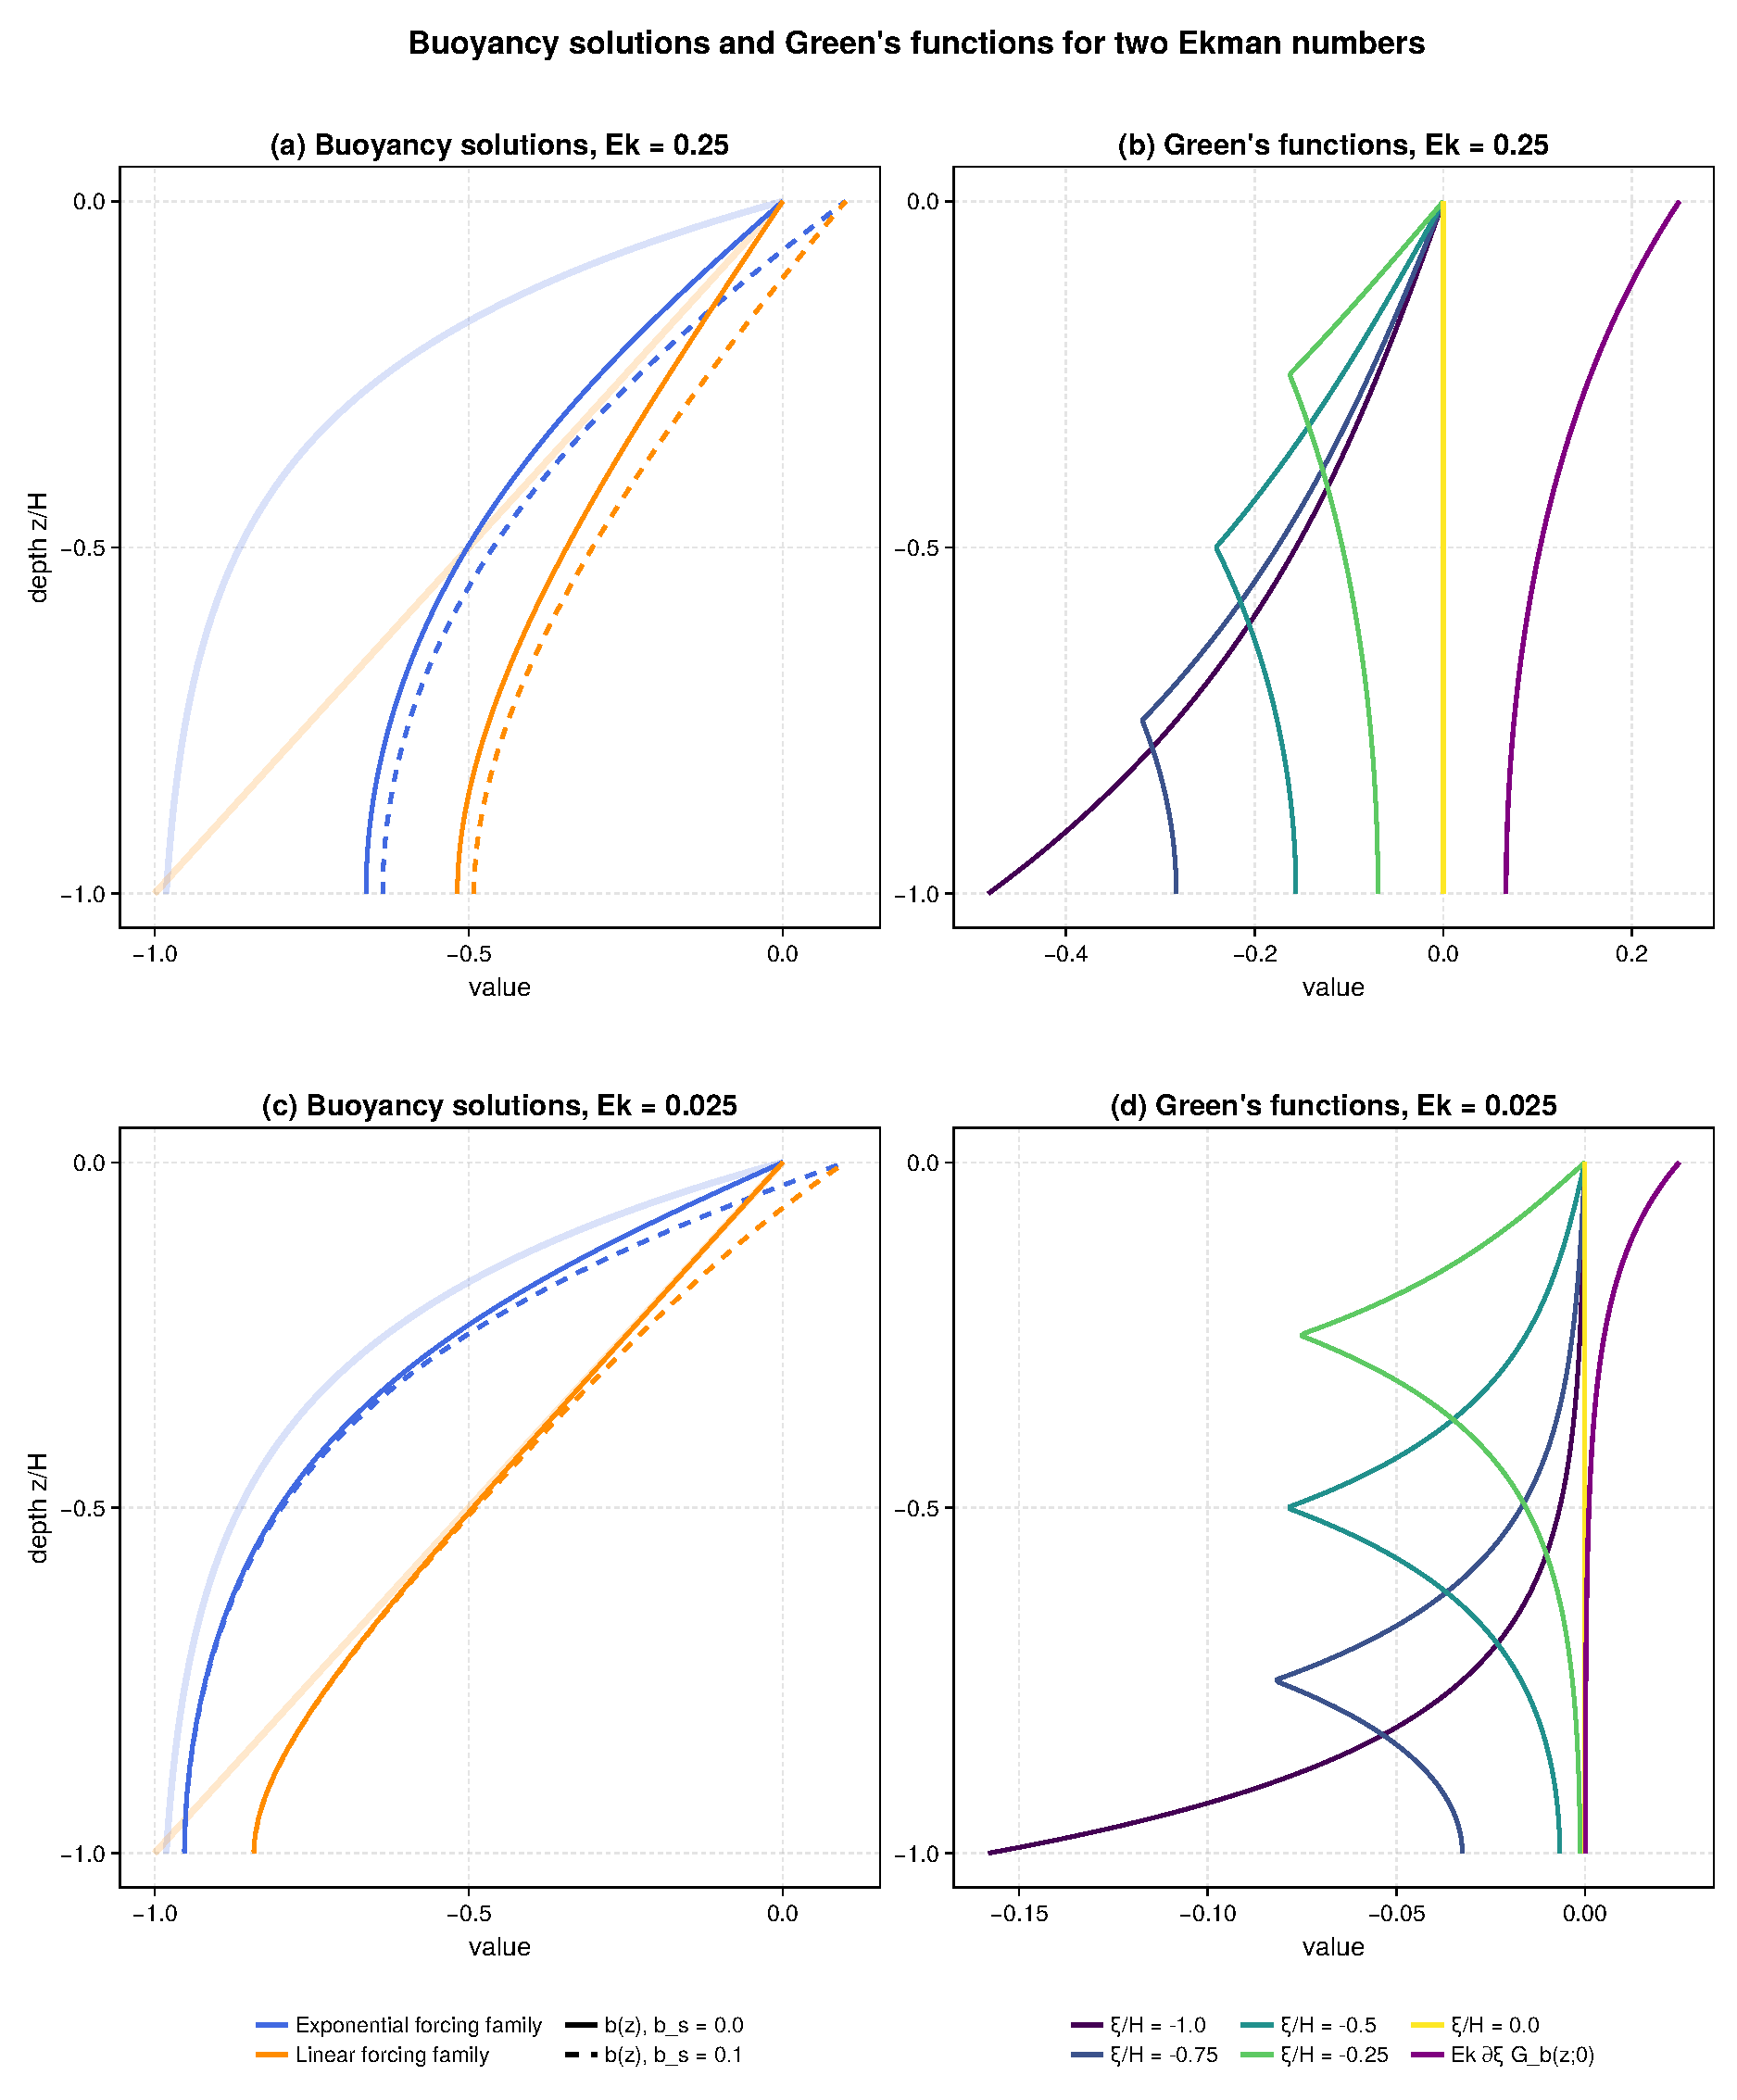
\includegraphics[width=14cm]{buoyancy_solutions_and_Greens_functions.pdf}
\caption{\label{fig:buoyancy_solutions} (a) and (c) Example solutions for buoyancy profiles $b(z)$ for various surface values $b_s$, forcing profiles $B(z)$ (faint colours), and Ekman numbers $\mathrm{Ek}$ (see (\ref{eqn:b_solution})). (b) and (d) show the corresponding Green's functions $G_b(z,\xi)$ for various source points $\xi$ (see (\ref{eqn:b_Greens_fn})). $H = \Gamma = \kappa = 1$ in this figure.}
\end{figure}

Examples of buoyancy solutions $b$ and buoyancy Green's functions $G_b$ are plotted in Figure \ref{fig:buoyancy_solutions}.
Two Ekman numbers are shown ($\mathrm{Ek} =$ 0.25 and 0.025), according to the row of the subplot, and $H = \Gamma = \kappa = 1$ (so $\psi = \mathrm{Ek}^{-1/2}$ here).
Four example $b$ profiles are shown for combinations of $b_s = 0$ and $b_s = 0.1$, and $B(z) = z$ and $B(z) = \mathrm{e}^{ 4 z/H} - 1$ (the $B(z)$ relaxation profiles are also plotted in Figure \ref{fig:buoyancy_solutions}a, c).
The $b$ solutions match the $b_s$ surface value and the no flux bottom boundary condition (\ref{eqn:simple_bot_b_bc}).
They are drawn towards the $B(z)$ profiles, especially for small $\mathrm{Ek}$, as expected from the buoyancy equation (\ref{eqn:steady_vertical_b}).
The $b$ profiles smoothly interpolate between these constraints.
Figure \ref{fig:buoyancy_solutions}b, d shows the $G_b(z; \xi)$ Green's functions for various $\xi$ source depths.
They are peaked (continuous with kinks) at $z = \xi$ with smaller magnitudes and narrower peaks for smaller Ekman number.
These functions weight the contribution from the relaxation profile $B$ in (\ref{eqn:b_solution}).
Figure \ref{fig:buoyancy_solutions} also shows the $\partial_\xi G_b(z;\xi) |_{\xi=0}$ functions from (\ref{eqn:dG_b_d_xi}).
They equal one at the surface and decay with depth, more rapidly for smaller Ekman number.
These functions multiply the surface boundary condition $b_s$ in (\ref{eqn:b_solution}). 



\begin{figure}
\centering
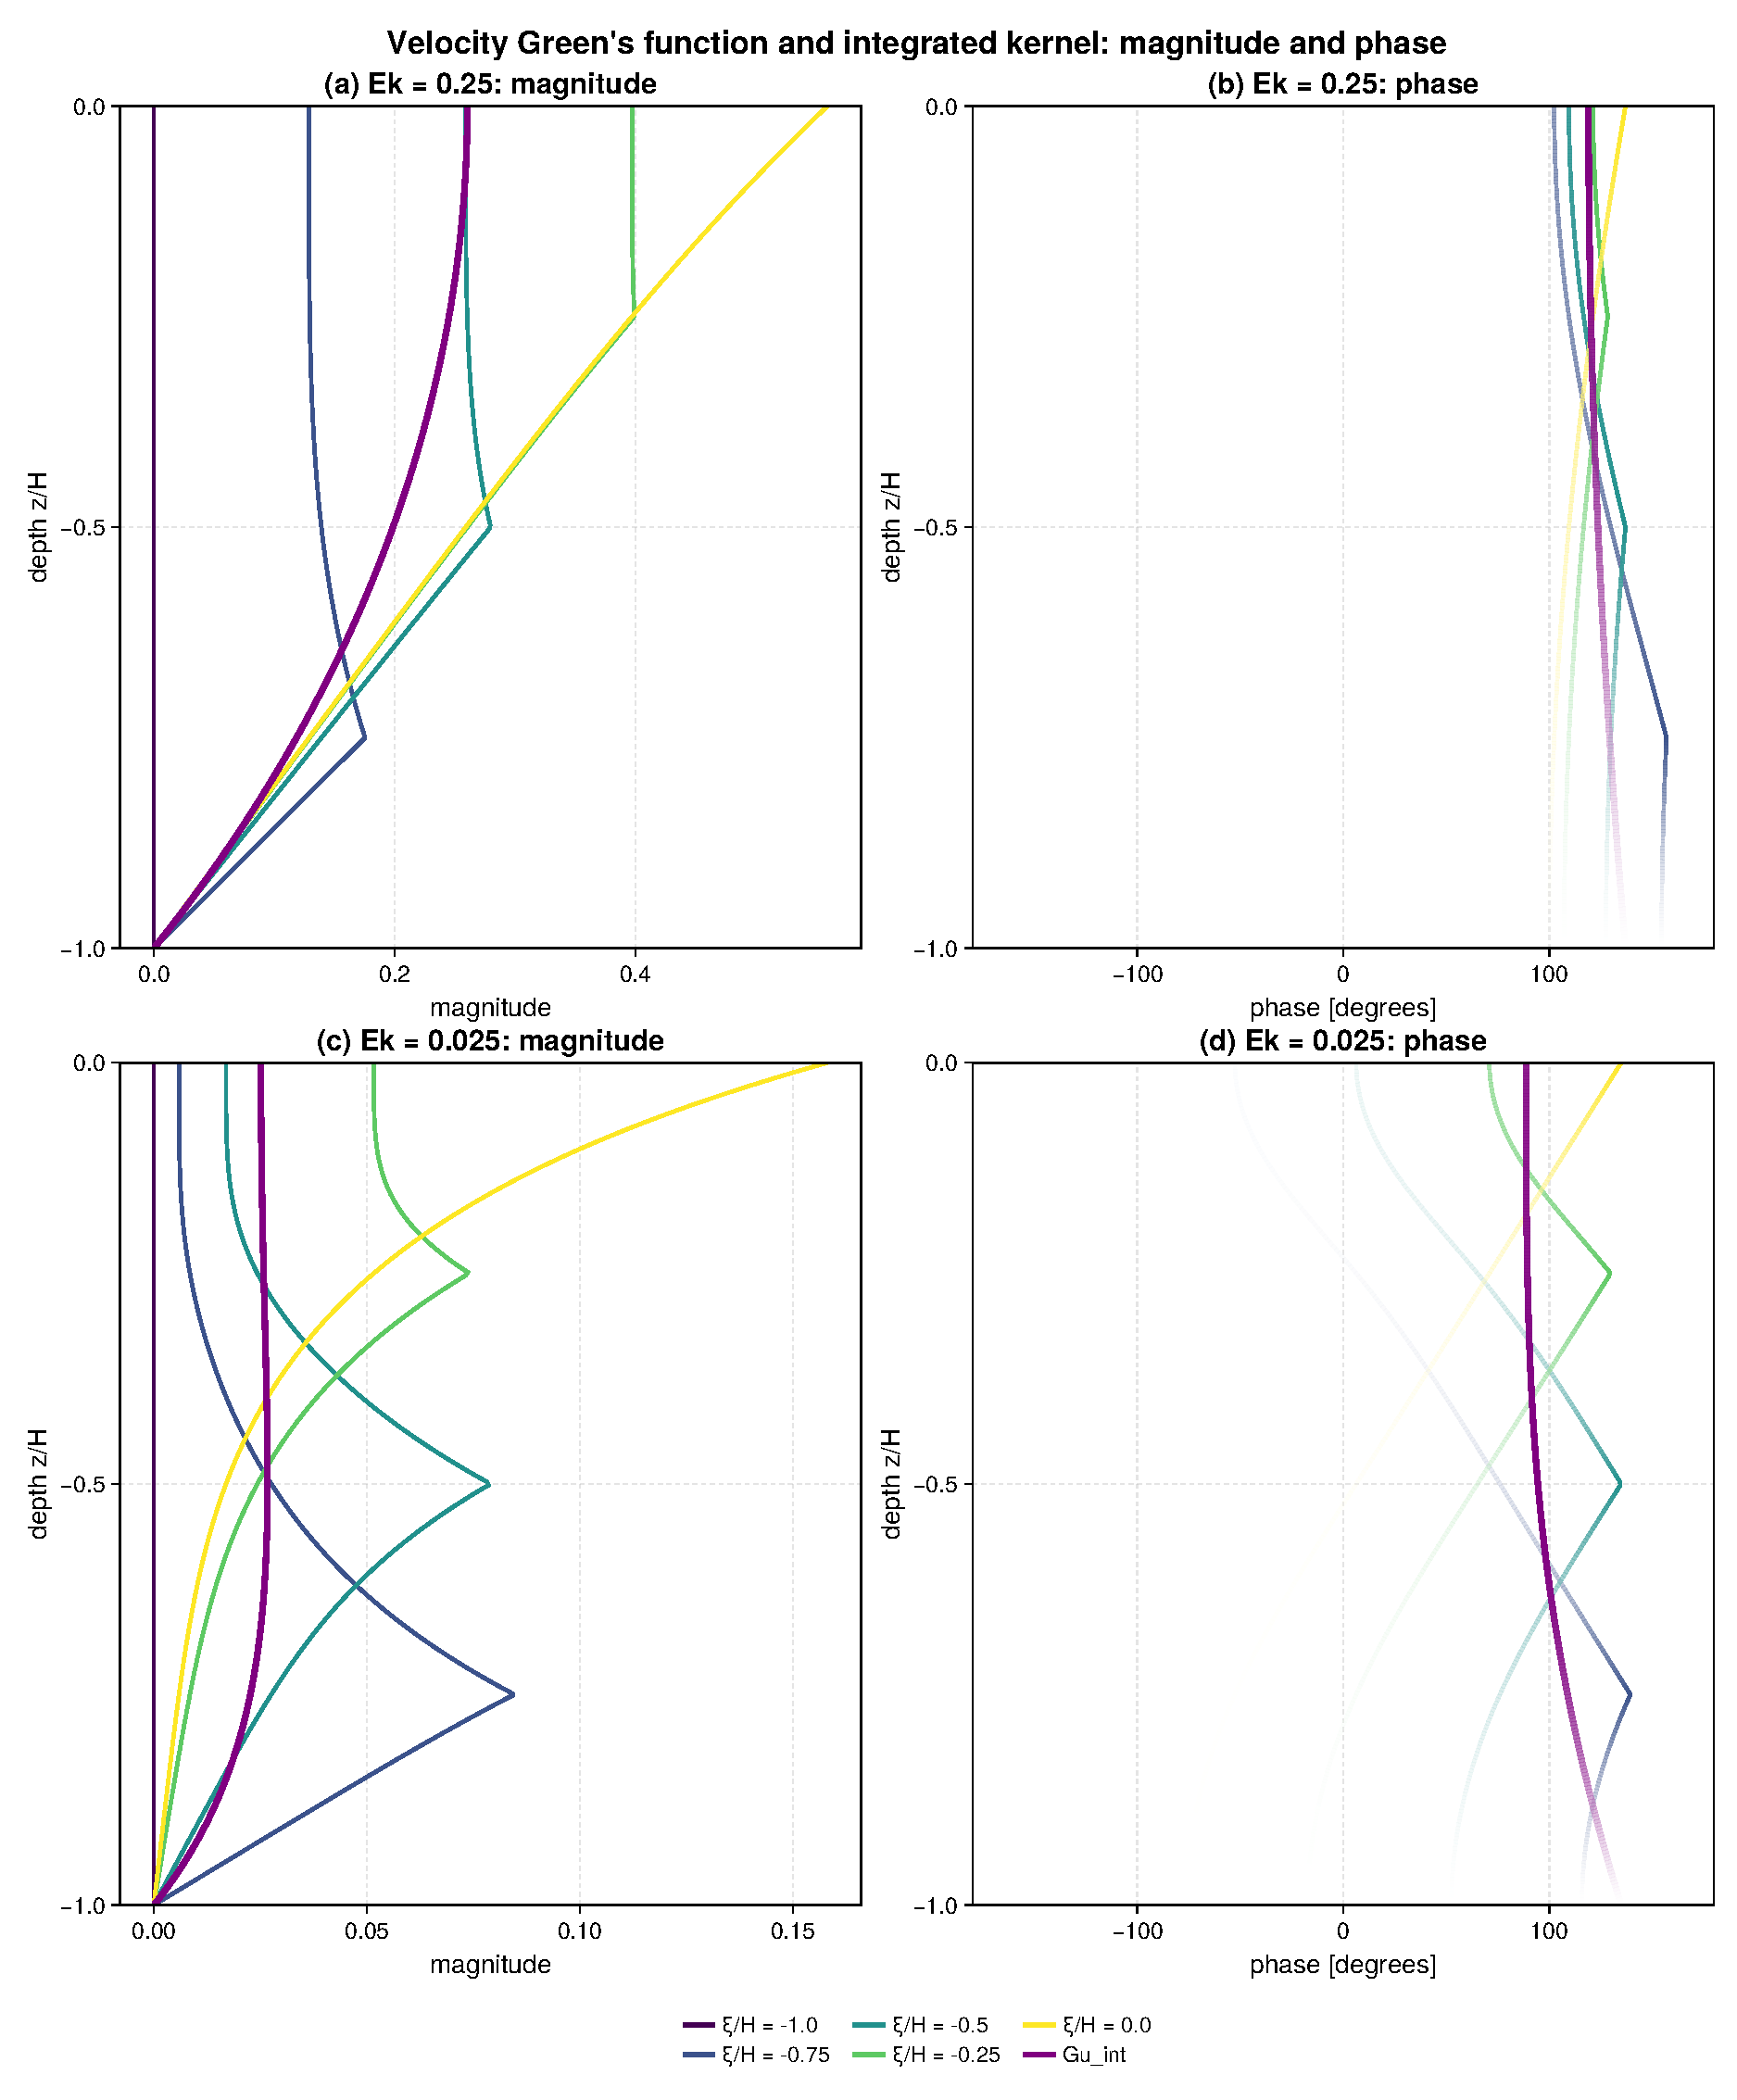
\includegraphics[width=14cm]{velocity_Gu_magnitude_phase_two_Ek.pdf}
\caption{\label{fig:velocity_Gsfn} Velocity Green's functions $G_{\mathfrak{u}}(z,\xi)$ for various source depths $\xi$ (see (\ref{eqn:FG_Gsfn})). (a) and (b) show the magnitude and phase, respectively, for $\mathrm{Ek} = 0.25$. (c) and (d) are the same, except for $\mathrm{Ek} = 0.025$. $H = f = \nu = 1$ in this figure, and the intensity of the phase colour is proportional to the corresponding magnitude of the Green's function component.
The Gu\_int quantity is $\int_{-H}^{0} G_{ \mathfrak{u}} (z; \xi) \; d \xi $.
See text for explanation of the phase convention.
}
\end{figure}

The horizontal velocity Green's function $G_\mathfrak{u}$ is plotted in Figure \ref{fig:velocity_Gsfn}.
Two Ekman numbers are shown ($\mathrm{Ek} =$ 0.25 and 0.025), according to the row of the subplot, and $H = f = \nu = 1$ (so $\phi = \mathrm{Ek}^{-1/2}$ here).
The $G_\mathfrak{u}$ magnitude is shown in the left column, and the phase in the right column.
Figure \ref{fig:velocity_Gsfn} also shows the vertically-integrated $G_\mathfrak{u}$ from (\ref{eqn:Guv_int_wrt_xi}).
To interpret these results, first consider the case of vanishing pressure gradient and surface stress in the positive $x$ direction (eastward; $\tau^y = 0$).
Eq.~(\ref{eqn:expanded_form_of_u}) shows that the surface velocity is then $- G_{\mathfrak{u}} (0; 0) \tau^x$.
The component $G_{\mathfrak{u}} (0; 0)$ is on the $\xi / H = 0$ curve, and has a phase of about 135$^\mathrm{o}$ for $\mathrm{Ek} = 0.025$ (Figure \ref{fig:velocity_Gsfn}d).
Therefore, $-G_{\mathfrak{u}} (0; 0)$ has a phase of -45$^\mathrm{o}$, which is measured anti-clockwise from the direction of the stress.
% Notebook cell reference, now summarized in the code-availability statement: (see \texttt{FrictionalGeostrophicEquationSolution.ipynb})
This corresponds to a surface current at 45$^\mathrm{o}$ to the right of the stress (in the northern hemisphere), consistent with small Ekman number theory \citep{salmon98,vallis06}.
Next consider the case of vanishing surface stress and an imposed surface pressure gradient in the positive $x$ direction (sea level slopes up to the east).
From (\ref{eqn:expanded_form_of_u}) the surface velocity is then proportional to $\int_{-H}^{0} G_{ \mathfrak{u}} (z; \xi) \; d \xi $.
The component $\int_{-H}^{0} G_{ \mathfrak{u}} (z; \xi) \; d \xi $ is labeled Gu\_int and has a phase of about 90$^\mathrm{o}$ for $\mathrm{Ek} = 0.025$ (Figure \ref{fig:velocity_Gsfn}d).
This corresponds to a surface geostrophic current flowing northwards with the pressure gradient force pushing westwards (opposite to the pressure gradient itself) and an equal and opposite Coriolis force pushing eastwards.
Finally, for the same case (no stress, $\partial_x p_s > 0 $), consider the bottom stress.
From (\ref{eqn:bottom_stress_ST_def}) and (\ref{eqn:S_fn}), 
$\tau_b$ is proportional to $(1/\varphi) \tanh \left( \varphi H \right)$.
Thus, as $\mathrm{Ek}$ gets small $\varphi = \sqrt{i f / \mathrm{Ek}} $ diverges, $\tanh \left( \varphi H \right) \rightarrow 1$ and $\tau_b$ becomes proportional to $i^{-1/2} = (1 - i)/\sqrt{2}$.
The bottom stress $1 - i$ corresponds to a southeast direction, which is at 135$^{\mathrm{o}}$ to the direction of the geostrophic current, consistent with textbook theory \citep{vallis06}.

These results establish the validity of the horizontal velocity Green's function $G_\mathfrak{u}$ in Figure \ref{fig:velocity_Gsfn} for familiar, special cases of (\ref{eqn:expanded_form_of_u}).
More generally, Figure \ref{fig:velocity_Gsfn} shows that $G_\mathfrak{u}$ respects the homogeneous velocity boundary conditions (\ref{eqn:sfc_bcs_frak}) and (\ref{eqn:bot_bcs_frak}) of vanishing vertical derivative at the surface and vanishing magnitude at the bottom (see (\ref{eqn:G_u_sfc_bc}) and (\ref{eqn:G_u_bot_bc})).
The kinked peaks at $z = \xi$ in $G_\mathfrak{u} (z; \xi )$ show how a pressure gradient causes a response in the horizontal velocity that is at 135$^{\mathrm{o}}$ to the pressure gradient; that is, at -45$^{\mathrm{o}}$ to the pressure gradient force (in the northern hemisphere).
Therefore, the water moves at 45$^{\mathrm{o}}$ to the right of the pressure gradient force.
This response decays with height above and below $z=\xi$ in clockwise spirals that represent internal Ekman layers.
The decay length scale depends inversely on the square root of the Ekman number, as expected.
The influence of the surface pressure gradient extends throughout the water column until it decays to zero in the bottom Ekman layer (Figure \ref{fig:velocity_Gsfn} Gu\_int curves).

\begin{figure}
\centering
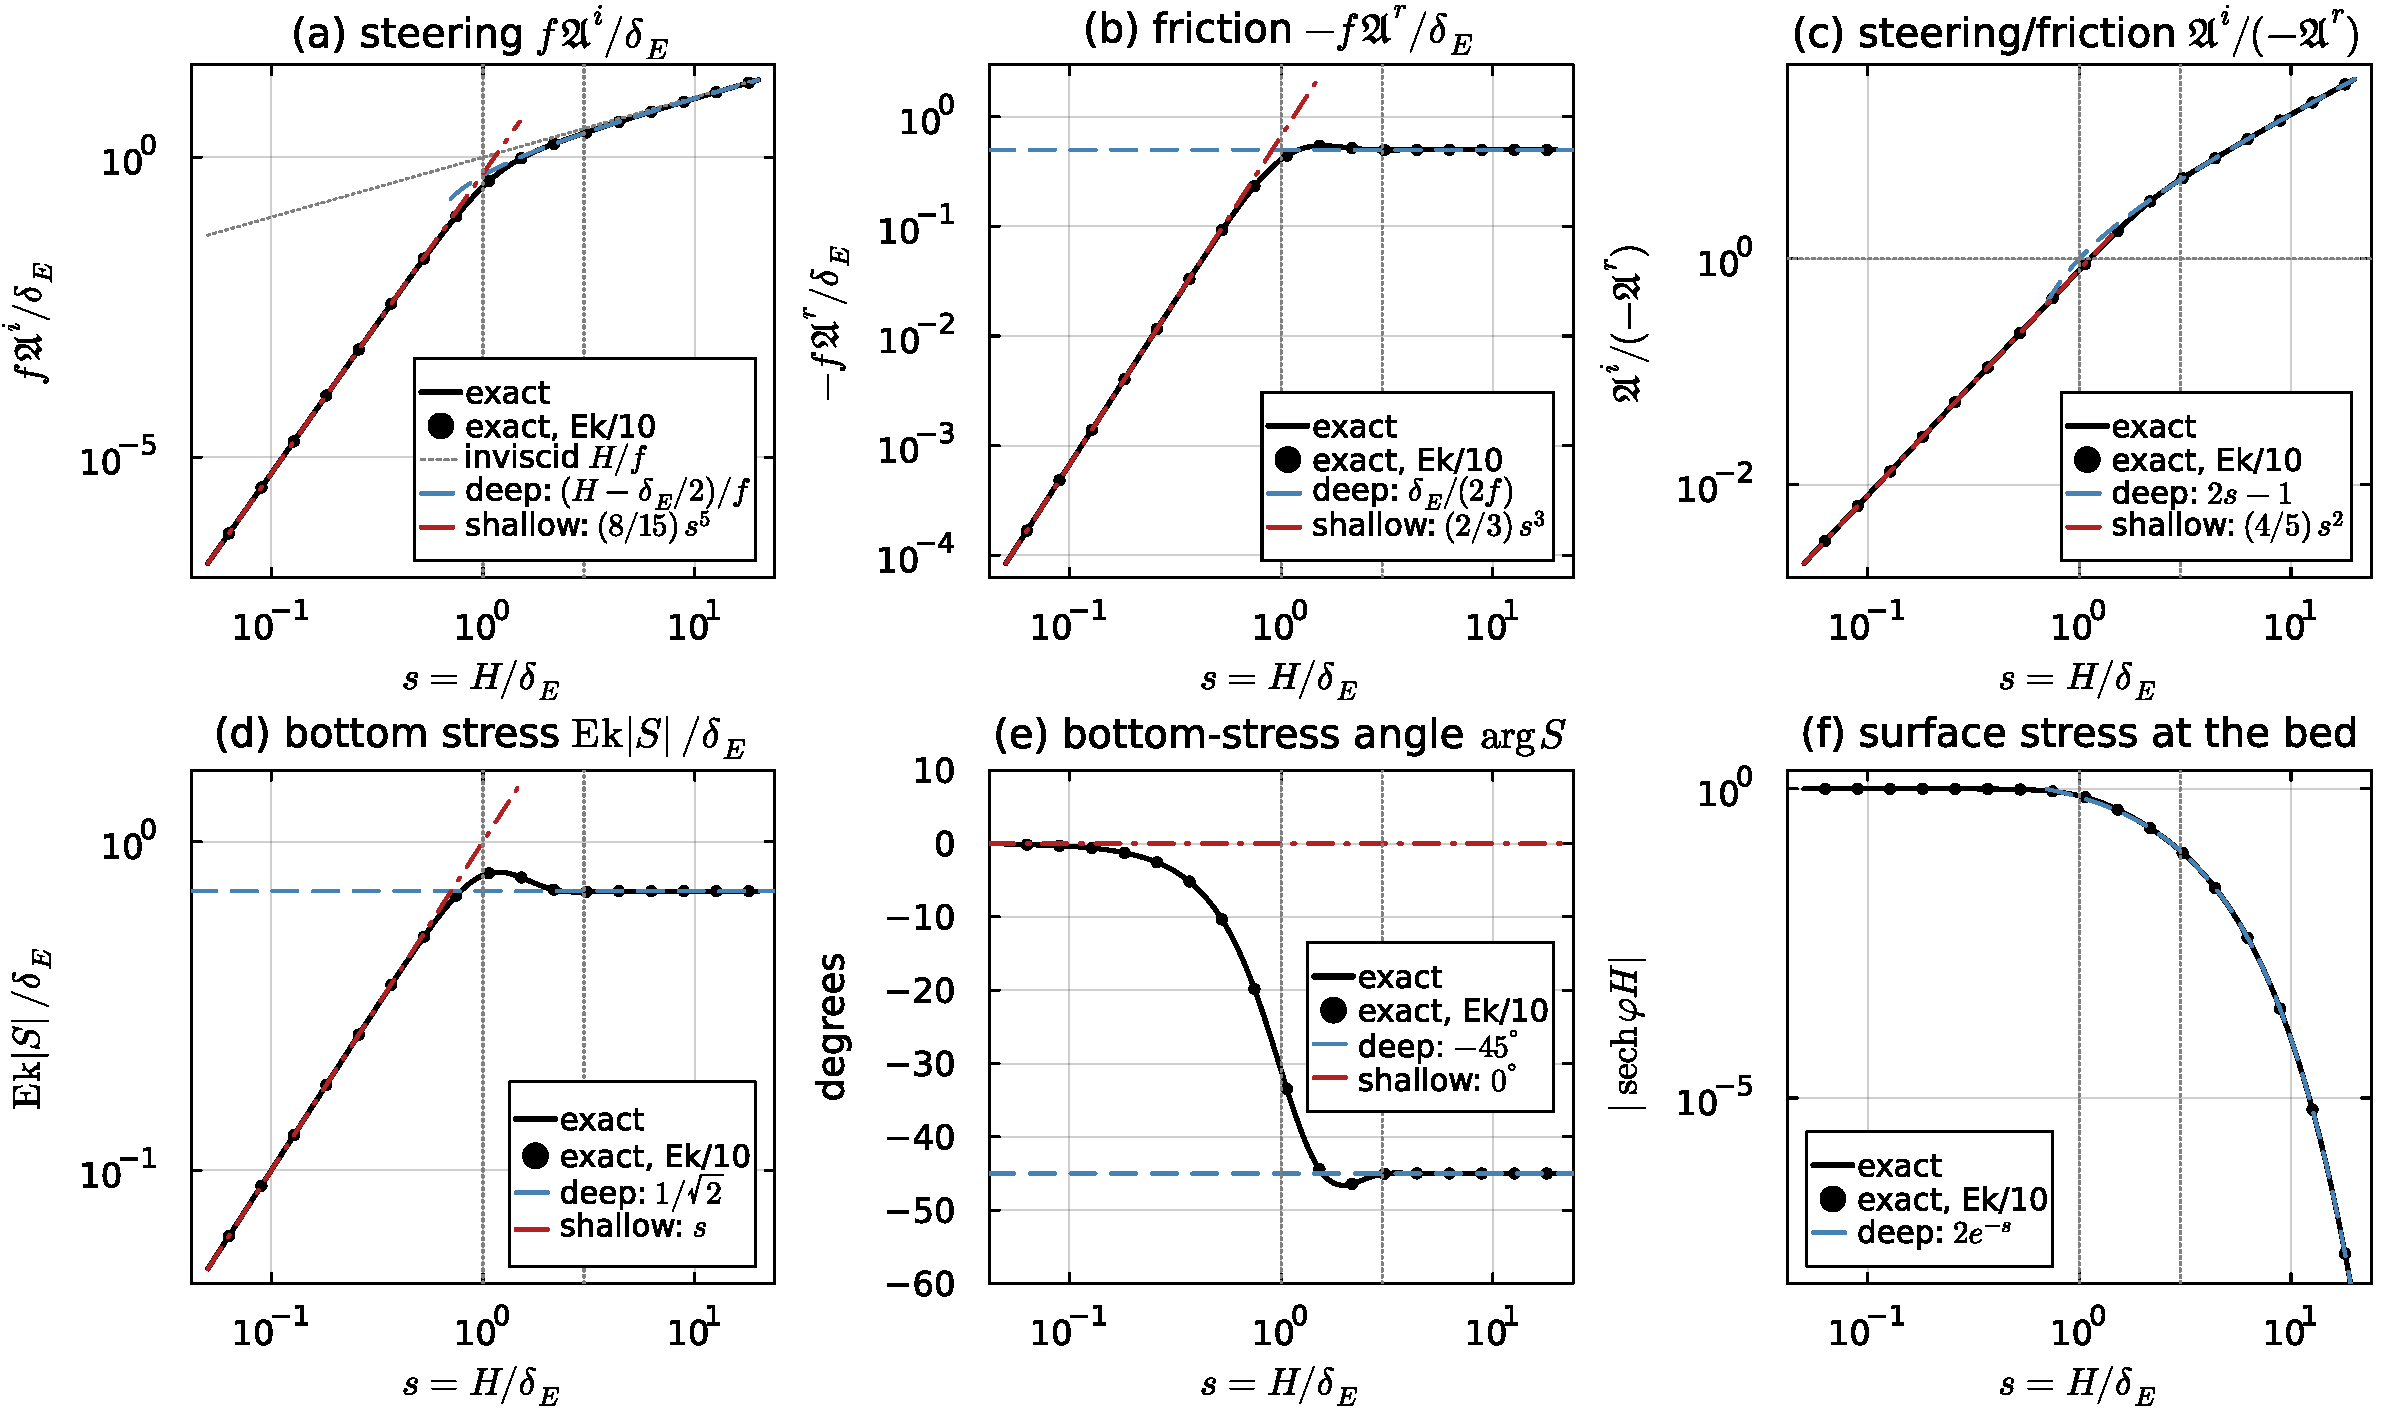
\includegraphics[width=16cm]{coefficient_regimes.pdf}
\caption{\label{fig:coefficient_regimes} Column coefficients against $s = H/\delta_E$, where $\delta_E = \sqrt{2 \nu \mathrm{Ek}/|f|}$ is the Ekman depth.
(a) Steering coefficient $f \mathfrak{A}^i/\delta_E$ from (\ref{eqn:A_fn}).
(b) Frictional diffusivity $-f \mathfrak{A}^r/\delta_E$.
(c) Their ratio $\mathfrak{A}^i/(-\mathfrak{A}^r)$.
(d) Magnitude and (e) angle of the bottom-stress coefficient $S$ from (\ref{eqn:S_fn}), scaled as $\mathrm{Ek}\,|S|/\delta_E$.
(f) Fraction of the surface stress that reaches the bed in $T$ (\ref{eqn:T_fn}), $|\mathrm{sech}\,\varphi H|$.
Solid curves use $\mathrm{Ek} = 10^{-2}$ and dots $\mathrm{Ek} = 10^{-3}$; the coefficients collapse because they depend only on $s$.
Dashed and dash-dotted lines are the deep ($s \gg 1$) and shallow ($s \ll 1$) asymptotes.
Dotted vertical lines mark $s = 1$ and $s = 3$.}
\end{figure}

\Claude{
With uniform viscosity the column coefficients depend on depth only through $s = H/\delta_E$, the depth measured in Ekman depths (Fig.~\ref{fig:coefficient_regimes}, $\delta_E = \sqrt{2 \nu \mathrm{Ek}/|f|}$ ).
For deep water ($s \gg 1$), $\mathfrak{A} \rightarrow [-\delta_E/2 + i(H - \delta_E/2)]/f$.
%\added[id=CL]{This limit and those below follow from (\ref{eqn:A_fn}) and (\ref{eqn:S_fn}) with $\varphi = (1 + i)/\delta_E$ (for $f > 0$ and $\nu = 1$, so that $\varphi^2 \mathrm{Ek} = i f$): $\tanh \varphi H \rightarrow 1$ for $s \gg 1$, and $\tanh(\varphi H)/(\varphi H) - 1 \approx -(\varphi H)^2/3 + 2 (\varphi H)^4/15$ for $s \ll 1$.
%The deep limits are the classical results for Ekman layers in water of finite depth \citep{ekman05, vallis06}.}
% Added by Claude (CL): TheoryNotes/PlotCoefficientRegimes.jl evaluates the exact
% coefficients (PlanetaryGeostrophy.pressure_coefficient and bottom_stress_coefficient),
% overlays these deep and shallow asymptotes in Fig. coefficient_regimes, and prints the
% relative errors of the deep limits at s = 1, 2, 3, 5 that are quoted below.
The depth-integrated flow is then the geostrophic transport over an effective depth $H - \delta_E/2$, plus a down-gradient bottom Ekman transport with diffusivity $\delta_E/(2f)$.
In other words, the surface pressure is advected along contours of $f/(H - \delta_E/2)$ and the bottom Ekman layer acts as a displacement thickness that modifies the classical $f/H$ steering (panel a).
The bottom-stress coefficient tends to $\mathrm{Ek}\,S \rightarrow \delta_E (1 - i)/2$, a linear drag rotated by $45^\circ$ (panels d, e), and the surface stress reaches the bed with weight $2e^{-s}$ (panel f).
These deep limits are accurate to better than 0.5\% for $s \geq 3$, the steering one to 0.15\% already at $s = 2$.
They reproduce classical Ekman-layer theory, including the linear bottom-drag coefficient $r = f \delta_E/(2H)$ of \citet{stommel48}.
For shallow water ($s \ll 1$), the Ekman layers overlap and $\mathfrak{A} \approx -H^3/(3\mathrm{Ek}) + i\,2 f H^5/(15\mathrm{Ek}^2)$.
The transport is then a lubrication flow down the surface-pressure gradient, proportional to $H^3$, and the bottom stress is aligned with that gradient.
Topographic steering is negligible: the ratio of steering to friction, $\mathfrak{A}^i/(-\mathfrak{A}^r)$, falls through one near $s \approx 1$ (panel c).
\added[id=CL]{Where the ocean is shallower than one to two Ekman depths,} therefore, $f/H$ contours no longer guide the depth-integrated flow, and classical layer models need the exact coefficients wherever $s \lesssim 3$.
}

\color{red}

\subsection{Verification}
\label{sect:verification}
The solution is verified at four levels: (i) agreement between independent evaluations of the analytical column solution, (ii) convergence of the finite-element surface-pressure solution as the mesh is refined, (iii) closure of the dynamical balances of Section~\ref{sect:dynamical_balances}, and (iv) comparison with an independent primitive-equation model.

\paragraph{Column solution.}
The horizontal velocity has three independent implementations.
The first is the direct double-quadrature form (\ref{eqn:final_velocity_formula1}).
The second is the symbolic-kernel form (\ref{eqn:final_velocity_formula2}).
The third, used in production, evaluates (\ref{eqn:appendix_fraku}), (\ref{eqn:T_fn}), and (\ref{eqn:B_fn}) as single vertical integrals of the closed-form kernels, with $\Pi(\xi)$ from (\ref{eqn:term1})--(\ref{eqn:term2}).
At a manufactured state with sloping bathymetry and a $\beta$-plane, the first two agree to a relative difference of $4 \times 10^{-11}$.
In a sloping, $\beta$-plane basin with a seamount and baroclinic forcing, the third agrees with the second to about $10^{-9}$ in $p_s$, $\mathbf{U}$, $\boldsymbol{\tau}_b$, $\Psi$, and $\mathbf{u}(z)$, and to $10^{-16}$ in $b$.
The remaining differences are set by the finite-difference step used for horizontal derivatives of $\Pi$.
\added[id=CL]{The three forms differ greatly in cost.
On one thread, a single velocity sample takes 3.8~ms with the first form and 0.26~ms with the second.
In the test basin on a mesh of size 0.04 and 18 threads, the surface-pressure solve takes 173~s with the second form and 0.5~s with the third, about 350 times faster, and sampling the velocity in 403 columns of 49 levels takes 0.63~ms and 0.063~ms per column (the script \texttt{TheoryNotes/ColumnMethodTimings.jl}).}

\paragraph{Mesh convergence.}
Figure~\ref{fig:verification_convergence}a and Table~\ref{tab:mesh_convergence} show the convergence of the solution as the surface-pressure mesh is refined.
The test basin is an ellipse with semi-axes 1 and 0.75 on a $\beta$-plane ($f = 1 + 0.15y$) with $\mathrm{Ek} = 0.01$ and $\Gamma = 0.2$.
Its depth field combines a uniform slope with a seamount and is $H \approx $0.54--1.06 at the coast, so the coast is a vertical wall and the no-normal-flow condition (\ref{eqn:ps_bc}) is active.
It is forced by surface stress, by surface buoyancy, and by a restoring buoyancy with depth-dependent horizontal gradients.
\added[id=CL]{The mesh size $h$ is the mean triangle edge length, which is within 3\% of the size requested from the mesh generator for requested sizes of 0.04 and below, 8\% smaller at 0.08, and 16\% smaller at 0.16.}
Errors are measured against the finest solution ($h = 0.010$) at 1341 points inside 97\% of the coastal radius.
With second-order Lagrange elements, the surface pressure and the streamfunction converge as $h^3$, and the transport, bottom stress, and interior velocity\added[id=CL]{, which depend on $\nabla p_s$,} as $h^2$.
\added[id=CL]{These are the optimal rates for this discretization.
The errors are not concentrated near the coast or its polygon vertices: the error in $\mathbf{U}$ over the inner half of the basin equals that over the whole basin.}
At $h = 0.020$ the relative error is $8 \times 10^{-6}$ in $p_s$ and about $2 \times 10^{-3}$ in $\mathbf{U}$ and $\boldsymbol{\tau}_b$.

\begin{table}
\caption{\label{tab:mesh_convergence} Relative $L_2$ error against the finest solution ($h = 0.010$) for the test basin of Section~\ref{sect:results}\ref{sect:verification}, with the observed order of convergence between successive meshes in parentheses.\added[id=CL]{ The mesh size $h$ is the mean triangle edge length.}}
\centering
\begin{tabular}{cccccc}
\hline
$h$ & $p_s$ & $\mathbf{U}$ & $\boldsymbol{\tau}_b$ & $\mathbf{u}(-H/2)$ & $\Psi$ \\
\hline
\added[id=CL]{0.134} & \added[id=CL]{$4.0 \times 10^{-3}$} & \added[id=CL]{$9.6 \times 10^{-2}$} & \added[id=CL]{$1.3 \times 10^{-1}$} & \added[id=CL]{$8.2 \times 10^{-2}$} & \added[id=CL]{$2.5 \times 10^{-2}$} \\
\added[id=CL]{0.074} & \added[id=CL]{$5.7 \times 10^{-4}$ (3.3)} & \added[id=CL]{$2.4 \times 10^{-2}$ (2.3)} & \added[id=CL]{$3.2 \times 10^{-2}$ (2.3)} & \added[id=CL]{$2.0 \times 10^{-2}$ (2.3)} & \added[id=CL]{$1.9 \times 10^{-3}$ (4.3)} \\
\added[id=CL]{0.039} & \added[id=CL]{$6.5 \times 10^{-5}$ (3.4)} & \added[id=CL]{$6.3 \times 10^{-3}$ (2.1)} & \added[id=CL]{$8.3 \times 10^{-3}$ (2.1)} & \added[id=CL]{$5.3 \times 10^{-3}$ (2.1)} & \added[id=CL]{$2.0 \times 10^{-4}$ (3.5)} \\
\added[id=CL]{0.020} & \added[id=CL]{$7.9 \times 10^{-6}$ (3.2)} & \added[id=CL]{$1.6 \times 10^{-3}$ (2.1)} & \added[id=CL]{$2.1 \times 10^{-3}$ (2.0)} & \added[id=CL]{$1.3 \times 10^{-3}$ (2.0)} & \added[id=CL]{$2.1 \times 10^{-5}$ (3.3)} \\
\hline
\end{tabular}
\end{table}

%\paragraph{Coastal boundary condition.}
%Imposing $p_s = 0$ on a vertical coastal wall, instead of (\ref{eqn:ps_bc}), lets frictional and buoyancy-forced transport cross the coast.
%In the double-basin example of Section~\ref{sect:results} (coast depth 0.26, $\mathrm{Ek} = 0.002$), the root-mean-square ratio of normal to tangential transport at 0.995 of the coastal radius is 0.37 with $p_s = 0$ and 0.02 with (\ref{eqn:ps_bc}).
%The relative difference between the transport $\mathbf{U}$ from (\ref{eqn:UV_AB_def}) and the transport $(-\partial_y \Psi, \partial_x \Psi)$ from the separately solved streamfunction (\ref{eqn:streamfunction_pde}) falls from 5\% to 0.05\% (mesh 0.02).

\paragraph{Dynamical balances.}
The depth-integrated momentum balance (\ref{eqn:U_mom})--(\ref{eqn:V_mom}) holds pointwise, because the column solution satisfies the momentum equations exactly.
Evaluated with centered differences of step $10^{-5}$ for $\nabla p_b$ and $\nabla \chi$, its relative residual is about \added[id=CL]{$10^{-5}$} in the double basin\added[id=CL]{ of Section~\ref{sect:results}\ref{sect:double_basin}, two deep bowls on an $f$-plane joined by a strait, with a shelf only four Ekman depths deep (Fig.~\ref{fig:double_basin_showcase})}.
The vorticity balances (\ref{eqn:BVE}), (\ref{eqn:DIV}), (\ref{eqn:GCVB}), and (\ref{eqn:TDVB}) are curls of that balance, so they also hold exactly for the continuous fields.\added[id=CR]{ For the present model the DIV balance is identical to the BV balance (Section~\ref{sect:dynamical_balances}), so it is not mapped separately.}
Mapping them requires care, however.
They act on the bottom stress and transport, which contain $\nabla p_s$, and with continuous Lagrange elements $\nabla p_s$ is discontinuous across element edges.
Centered differences of these fields therefore do not converge: their relative residual stays at 0.95--1.04 for every mesh in Fig.~\ref{fig:verification_convergence}b, and at \added[id=CL]{0.73--1.0} on every diagnostic grid in the double basin\added[id=CL]{, from $17 \times 17$ to $129 \times 129$}.
Instead we average each term over the diagnostic cell around each grid point.
By Stokes' theorem, $\iint \hat{\mathbf{z}} \cdot \nabla \times \mathbf{F} \, dA = \oint \mathbf{F} \cdot \hat{\mathbf{t}} \, ds$ and $\iint J(a,b) \, dA = \oint a \, \nabla b \cdot \hat{\mathbf{t}} \, ds$, so every curl and Jacobian becomes an edge integral, for example $\oint p_b \, dH$ for the bottom-pressure torque.
The advection terms $U \partial_x f + V \partial_y f$ and $J(f/H, \Psi) = -\mathbf{U} \cdot \nabla (f/H)$ use area quadrature.
No finite-element field is differentiated.
Setting $\nabla \cdot \mathbf{U} = 0$ as in (\ref{eqn:BVE_constraint}), each cell-averaged residual equals the cell-averaged finite-element mass-conservation error: $-f \nabla \cdot \mathbf{U}$ for the BV and DIV balances, $(f/H) \nabla \cdot \mathbf{U}$ for the GCVB, and $-\nabla \cdot \mathbf{U}$ for the TDVB.
These residuals converge under mesh refinement\added[id=CL]{, at roughly $h^2$ once $h \lesssim 0.04$}, from 0.61 (BV) and 0.30 (GCVB) at $h = 0.13$ to $2.0 \times 10^{-3}$ and $7 \times 10^{-4}$ at $h = 0.010$ (Fig.~\ref{fig:verification_convergence}b).
\added[id=CL]{In the double basin the cell-averaged residuals are $4 \times 10^{-3}$ (BV) and $8 \times 10^{-3}$ (GCVB) on a $17 \times 17$ grid, and grow to 0.10 and 0.08 on a $129 \times 129$ grid, whose cells are smaller than the finite elements, so that the mass-conservation error of each element is less averaged out.}
In the double basin, integrating the GCVB over the regions enclosed by closed $f/H$ contours, as in (\ref{eqn:integrated_GCVB}), closes to $3 \times 10^{-3}$ of its terms.
The stress circulation around closed isobaths closes to $6 \times 10^{-4}$.
The area-integrated GCVB over the northern and southern halves of the basin, either side of the strait, closes to \added[id=CL]{$4.5 \times 10^{-5}$ and $1.2 \times 10^{-4}$}.

\paragraph{Comparison with a primitive-equation model.}
Appendix~C compares the solution with \texttt{Oceananigans.jl} \citep{wagner_etal25}, whose hydrostatic free-surface model is integrated from rest to a steady state with momentum and buoyancy advection switched off.
The test uses an elliptical basin on a $\beta$-plane with $\mathrm{Ek} = 0.02$, a flat bottom of depth 0.65 bounded by a vertical coastal wall, weak zonal surface stress, and spatially varying surface and restoring buoyancy.
The two models then solve the same linear equations and differ only in their discretizations.
Away from the coast and the bottom, the relative $L_2$ difference in the depth-integrated transport $\mathbf{U}$ is 11\%, 4.3\%, and 1.5\% on $40 \times 30 \times 20$, $80 \times 60 \times 40$, and $160 \times 120 \times 40$ \texttt{Oceananigans.jl} grids, and in the horizontal velocity $\mathbf{u}$ it is 8.0\%, 3.4\%, and 1.1\% (Fig.~\ref{fig:oceananigans_comparison}).
This is roughly first-order convergence in the horizontal grid spacing, consistent with the stair-stepped immersed coastline of the \texttt{Oceananigans.jl} grid.
The buoyancy differences are $1.5 \times 10^{-3}$, $3.5 \times 10^{-4}$, and $3.5 \times 10^{-4}$, limited by the vertical resolution.
Unlike buoyancy, which is column-local, $\mathbf{u}$ and $\mathbf{U}$ test the surface-pressure solve and the coastal condition.
The PG solution takes about a second to compute, 25 to 150 times faster than the \texttt{Oceananigans.jl} run (Appendix~C).

\begin{figure}
\centering
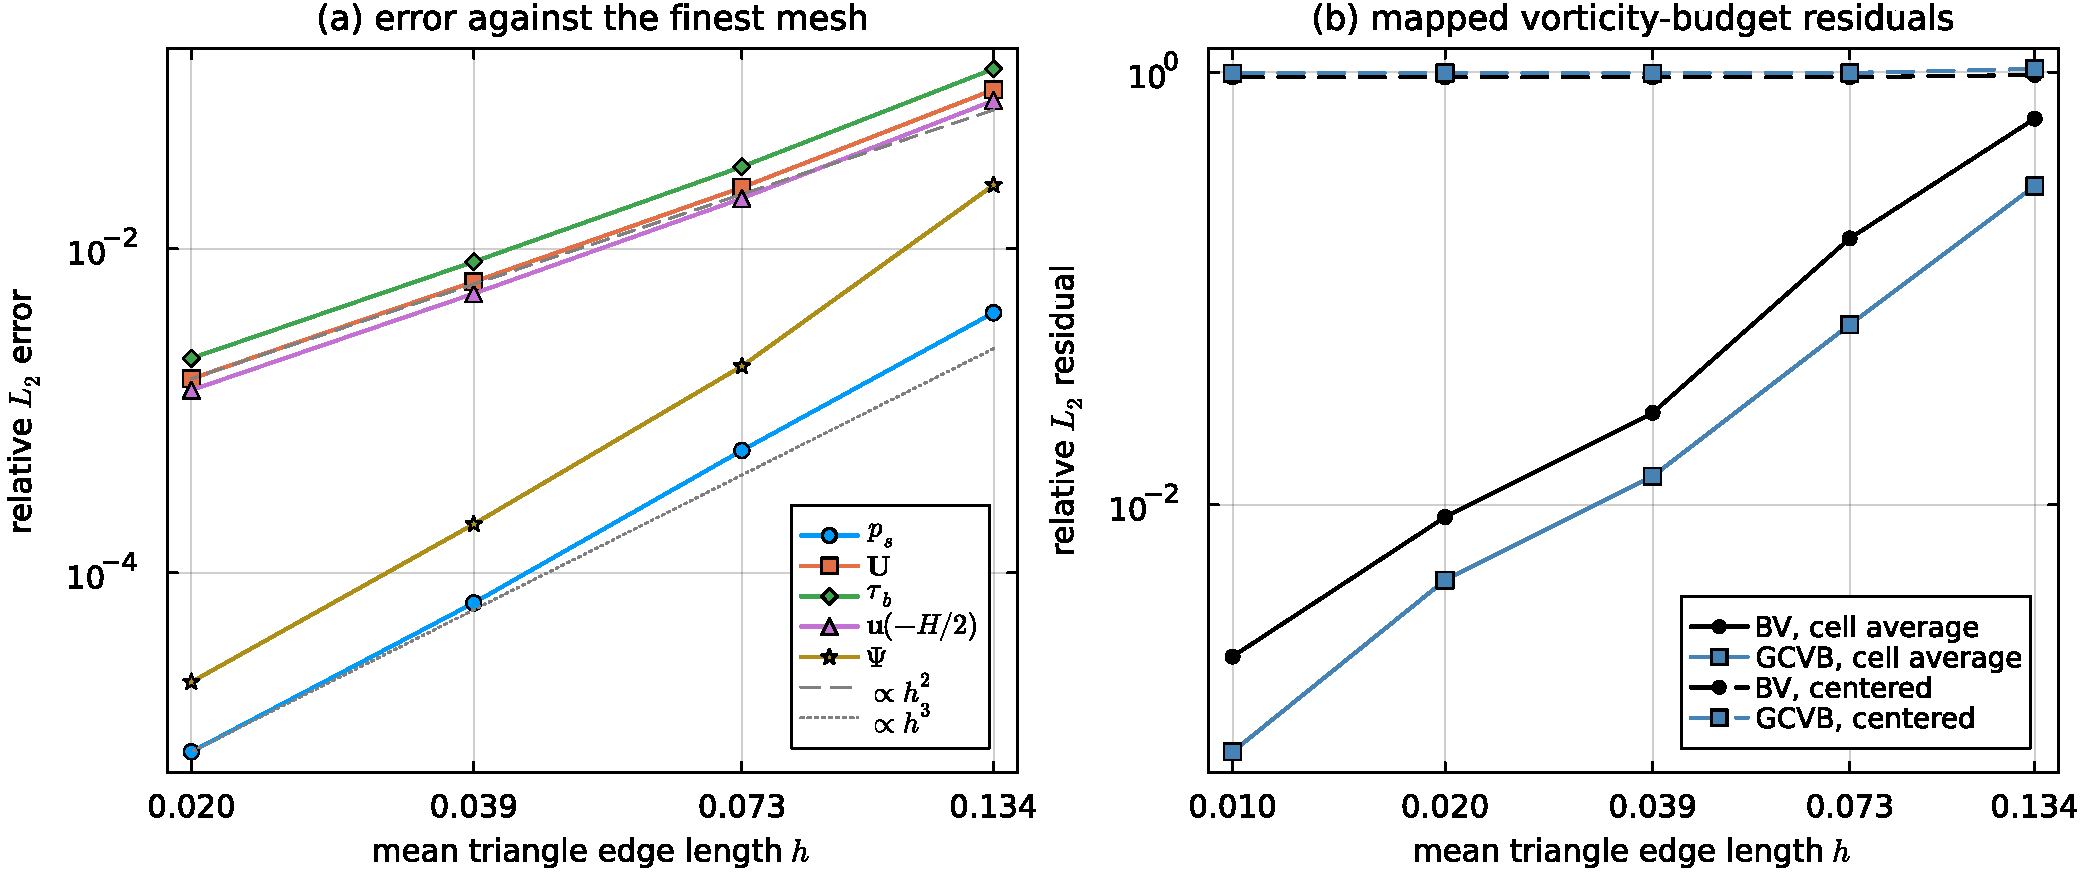
\includegraphics[width=16cm]{verification_convergence.pdf}
\caption{\label{fig:verification_convergence} Verification in the test basin of Section~\ref{sect:results}\ref{sect:verification}.
(a) Relative $L_2$ error against the finest solution ($h = 0.010$) as the surface-pressure mesh is refined, for the surface pressure $p_s$, depth-integrated transport $\mathbf{U}$, bottom stress $\boldsymbol{\tau}_b$, velocity at mid-depth, and streamfunction $\Psi$\added[id=CL]{; $h$ is the mean triangle edge length}. Gray lines show $h^2$ and $h^3$.
(b) Relative residuals of the mapped barotropic (BV, (\ref{eqn:BVE})) and geostrophic-contour (GCVB, (\ref{eqn:GCVB})) vorticity balances on a fixed $19 \times 15$ diagnostic grid. Solid lines: cell averages via Stokes' theorem. Dashed lines: centered differences of the sampled fields.}
\end{figure}

\color{black}

%Useful for comparison: \citet{willmott&luneva15}


% Added by Claude (CL): Section 6c, classical limits. Made by TheoryNotes/StommelComparison.jl.
\subsection{Classical limits}
\label{sect:classical_limits}

\paragraph{\added[id=CL]{Sverdrup interior and Stommel boundary layer.}}
\added[id=CL]{A flat rectangular basin ($2 \times 1$, $H = 1$) on a $\beta$-plane, $f = 1 + 0.6\,y$, is forced by the zonal wind $\tau^x = -\tau_0 \cos (\pi \eta)$, with $\eta = y + 1/2$, and has no buoyancy forcing.
The classical model is that of \citet{stommel48}, $r \nabla^2 \Psi + \beta \partial_x \Psi = \mathrm{Ek}\, \hat{\mathbf{z}} \cdot \nabla \times \boldsymbol{\tau}$ with $\Psi = 0$ on the coast, whose solution separates as $\Psi = X(x) \sin (\pi \eta)$.
Its drag coefficient is not fitted: $r = f_0 \delta_E/(2H)$ is the deep limit of the PG bottom stress (Section~\ref{sect:results}a).
The PG streamfunction is integrated from the PG transport, $\Psi = -\int_x^{x_E} V \, dx'$, independently of the streamfunction solve (\ref{eqn:streamfunction_pde}).
For $s = H/\delta_E = 28$, 14, 7, and 3.5 ($\mathrm{Ek}$ from $6.25 \times 10^{-4}$ to 0.04), the relative $L_2$ difference in $\Psi$ is 2.6\%, 3.3\%, 5.3\%, and 8.0\%.
PG reproduces both the Sverdrup interior and the western boundary layer of width $r/\beta$ (Fig.~\ref{fig:stommel_comparison}).
Two corrections, both implied by the PG bottom stress, account for most of the remaining difference.
First, the Ekman drag varies with latitude, $r(y) = f \delta_E/(2H) \propto f^{1/2}$; with this local drag the difference falls to 1.0\% and 1.2\% for $s = 28$ and 14.
Second, the bottom Ekman layer acts as a displacement thickness, so the drag acts on the velocity $\mathbf{U}/(H - \delta_E/2)$; with both corrections the difference at $s = 7$ falls from 5.3\% to 1.5\%.
The remaining 1\% is comparable to the error of evaluating the corrected model row by row, which neglects $\partial_y r$.
At $s = 3.5$ neither correction helps (7\%): the Ekman layers fill much of the column, the wind stress reaches the bed with weight $2 e^{-s} \approx 6\%$, and a layer model needs the exact coefficients $\mathfrak{A}$ and $S$ (Fig.~\ref{fig:coefficient_regimes}).}

\begin{figure}
\centering
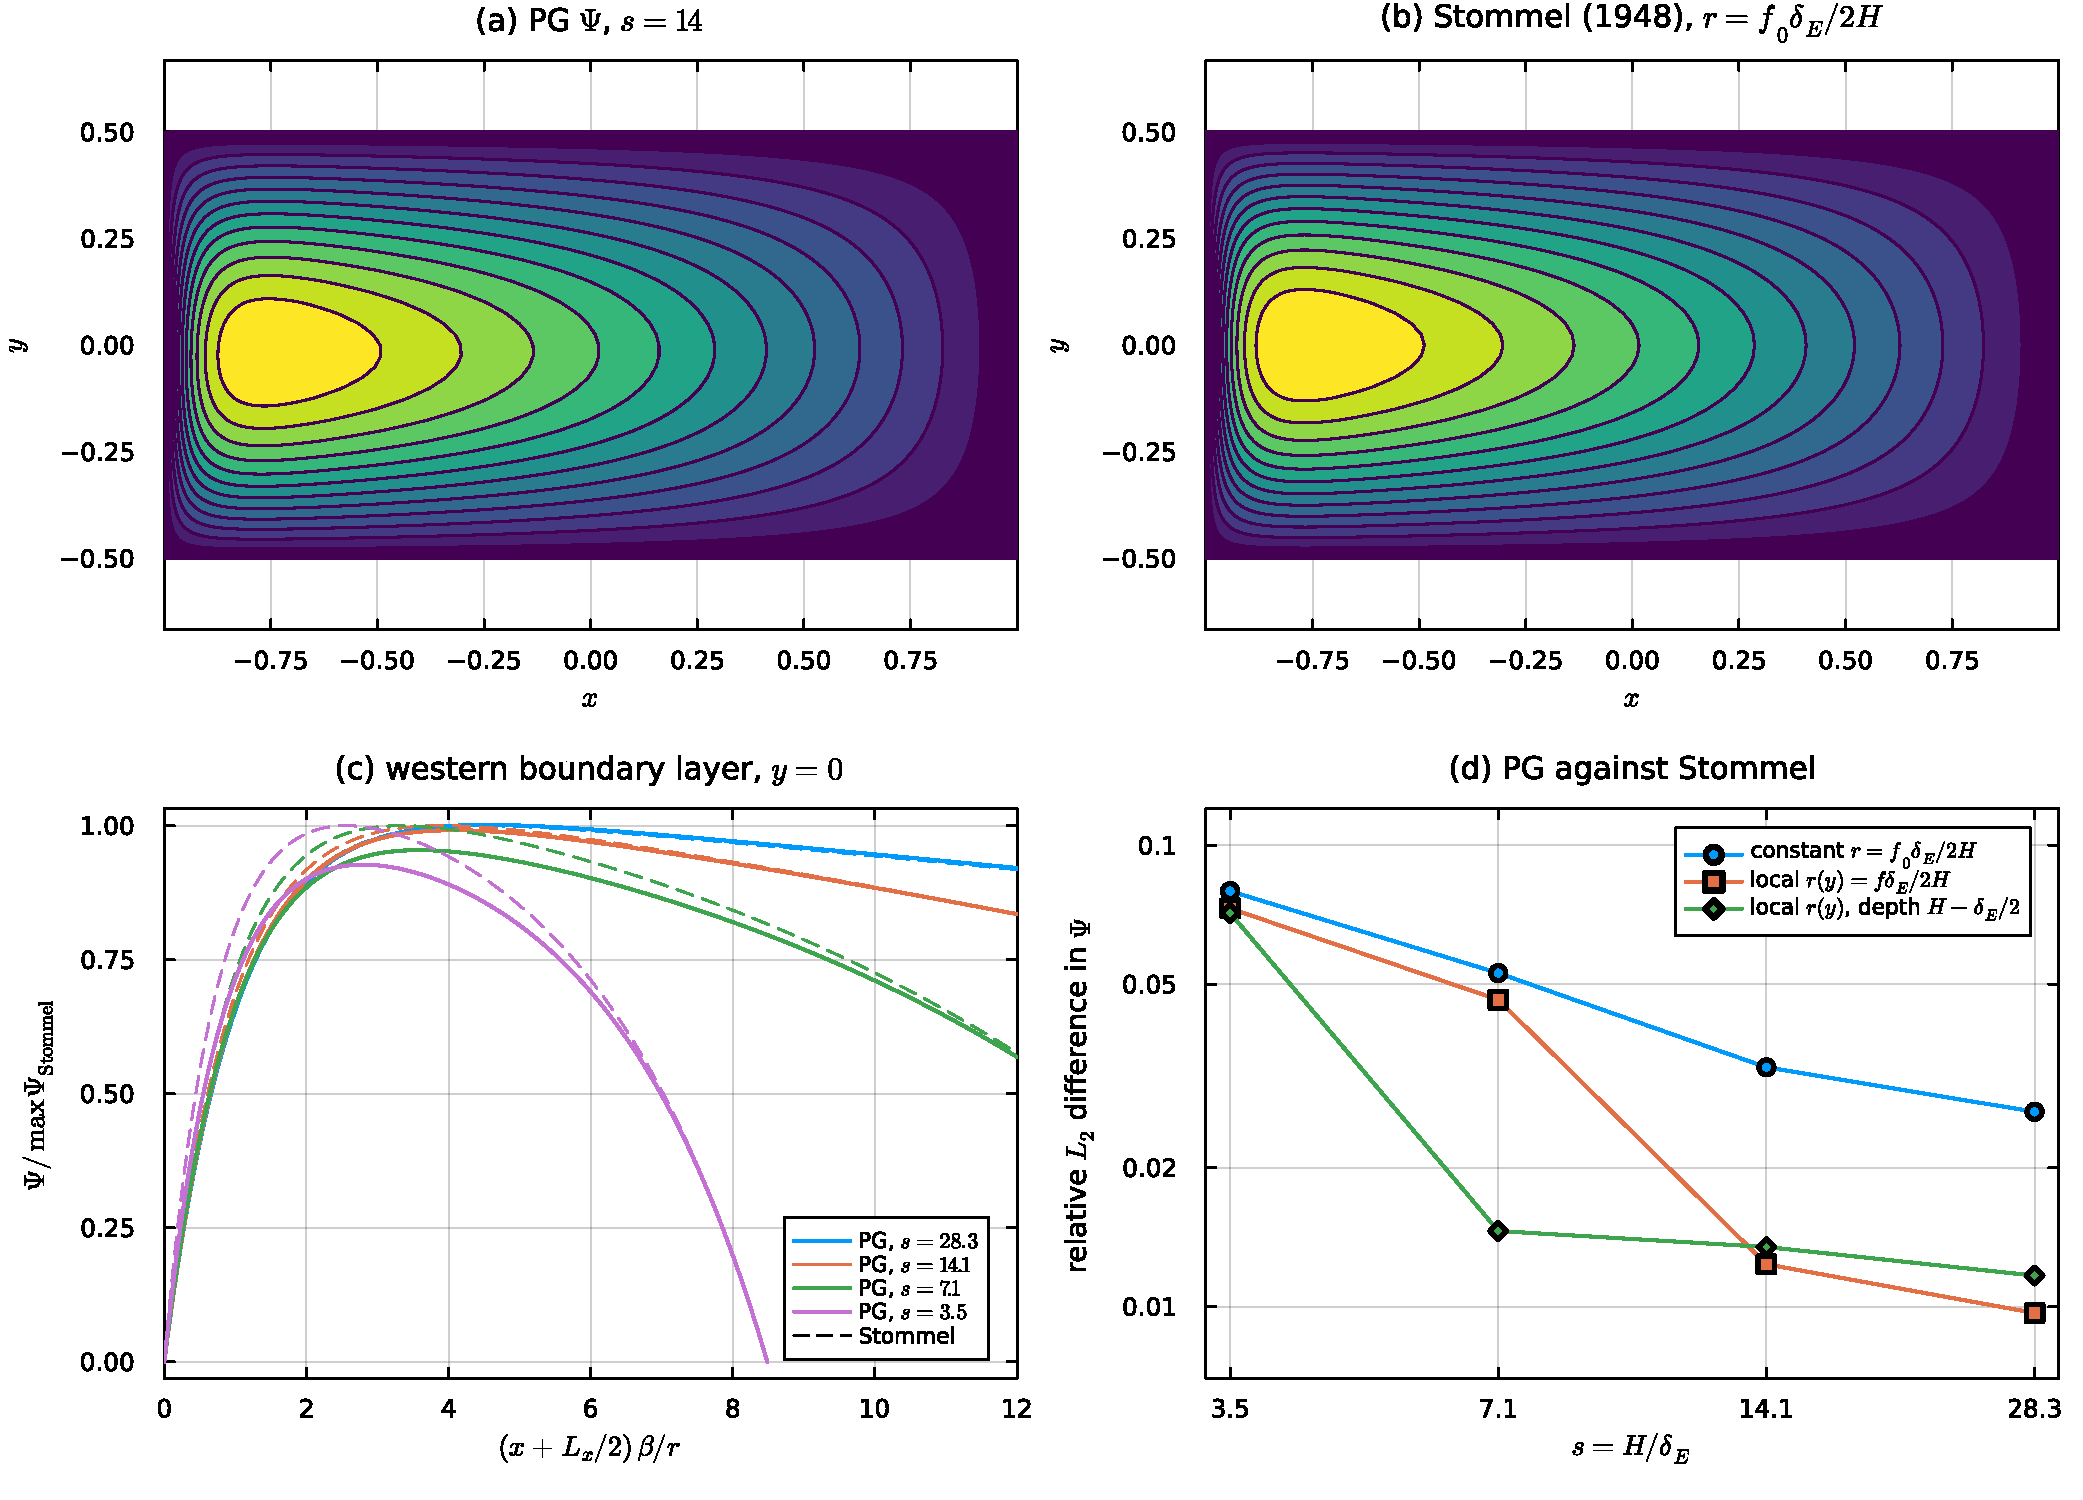
\includegraphics[width=14cm]{stommel_comparison.pdf}
\caption{\added[id=CL]{\label{fig:stommel_comparison} Sverdrup interior and Stommel western boundary layer.
(a) PG streamfunction $\Psi$ for $s = H/\delta_E = 14$ ($\mathrm{Ek} = 2.5 \times 10^{-3}$), and (b) the \citet{stommel48} solution with the derived drag $r = f_0 \delta_E/(2H)$, on the same contour levels.
(c) Zonal profiles of $\Psi$ at $y = 0$ across the western boundary layer, against distance in units of $r/\beta$, for four values of $s$: PG (solid) and Stommel (dashed), normalized by the Stommel maximum.
(d) Relative $L_2$ difference between the PG and Stommel $\Psi$ against $s$, for the classical constant drag, for the local drag $r(y) = f \delta_E/(2H)$, and for the local drag acting over the depth $H - \delta_E/2$.}}
\end{figure}

\paragraph{\added[id=CL]{$\beta$ plumes.}}
\added[id=CL]{An isolated Gaussian patch of positive wind-stress curl, of radius 0.2, in a flat $4 \times 2$ basin with $f = 1 + 0.3\,y$ drives the westward $\beta$ plume of \citet{stommel82}.
The classical model is the frictional vorticity equation $\nabla \cdot (r \nabla \Psi) + \beta \partial_x \Psi = \mathrm{Ek}\, \hat{\mathbf{z}} \cdot \nabla \times \boldsymbol{\tau}$ with $\Psi = 0$ on the coast, solved by second-order finite differences in the same basin, so that the walls and a variable drag are treated exactly.
With the constant derived drag $r = f_0 \delta_E/(2H)$, the relative $L_2$ difference in $\Psi$ is 1.5\%, 2.7\%, 6.5\%, and 8.8\% for $s = 26$, 13, 6.5, and 3.2.
With the local Ekman drag acting over the displacement thickness, $r(y) = f \delta_E/[2(H - \delta_E/2)]$, it is 0.8\%, 1.3\%, 1.9\%, and 9.1\% (Fig.~\ref{fig:beta_plume_comparison}).
As for the gyre, these two corrections, both implied by the PG bottom stress, halve the difference or better wherever $s \gtrsim 6$, and the layer model fails near $s \approx 3$.}

\added[id=CL]{\citet{haine&fuller16} give the exact solution for a $\beta$ plume beside a straight coast inclined at angle $\theta$ to east--west, with Rayleigh drag $\lambda$: the free-space plume of the source minus a weighted image source reflected in the coast.
In a basin cut by such a coast, a Gaussian source of radius 0.1 lies $5 \delta_S$ from it, where $\delta_S = \lambda/\beta$ is the Stommel length and $\lambda = f_0 \delta_E/(2H)$ is again derived ($s = 62$; $\beta = 0.1$, }\added[id=CL]{so that the drag varies by less than about 10\% over the domain}\added[id=CL]{).
PG reproduces the exact solution, convolved with the source, to 0.7\% for $\theta = 30^\circ$ and 0.6\% for $\theta = 60^\circ$ (Fig.~\ref{fig:boundary_beta_plume_comparison}).
Down-plume, along the line through the source parallel to the coast, the PG e-folding length (fitted after removing }\added[id=CL]{the $d^{-3/2}$ factor of the far-field asymptote, with $d$ the down-plume distance}\added[id=CL]{) is within 7\% and 3\% of that of the exact solution.
Within the basin neither has yet reached the asymptotic e-folding length $2 \delta_S/(1 - \cos \theta)$.
This test also exercises the no-normal-flow condition on an inclined coast.}

\begin{figure}
\centering
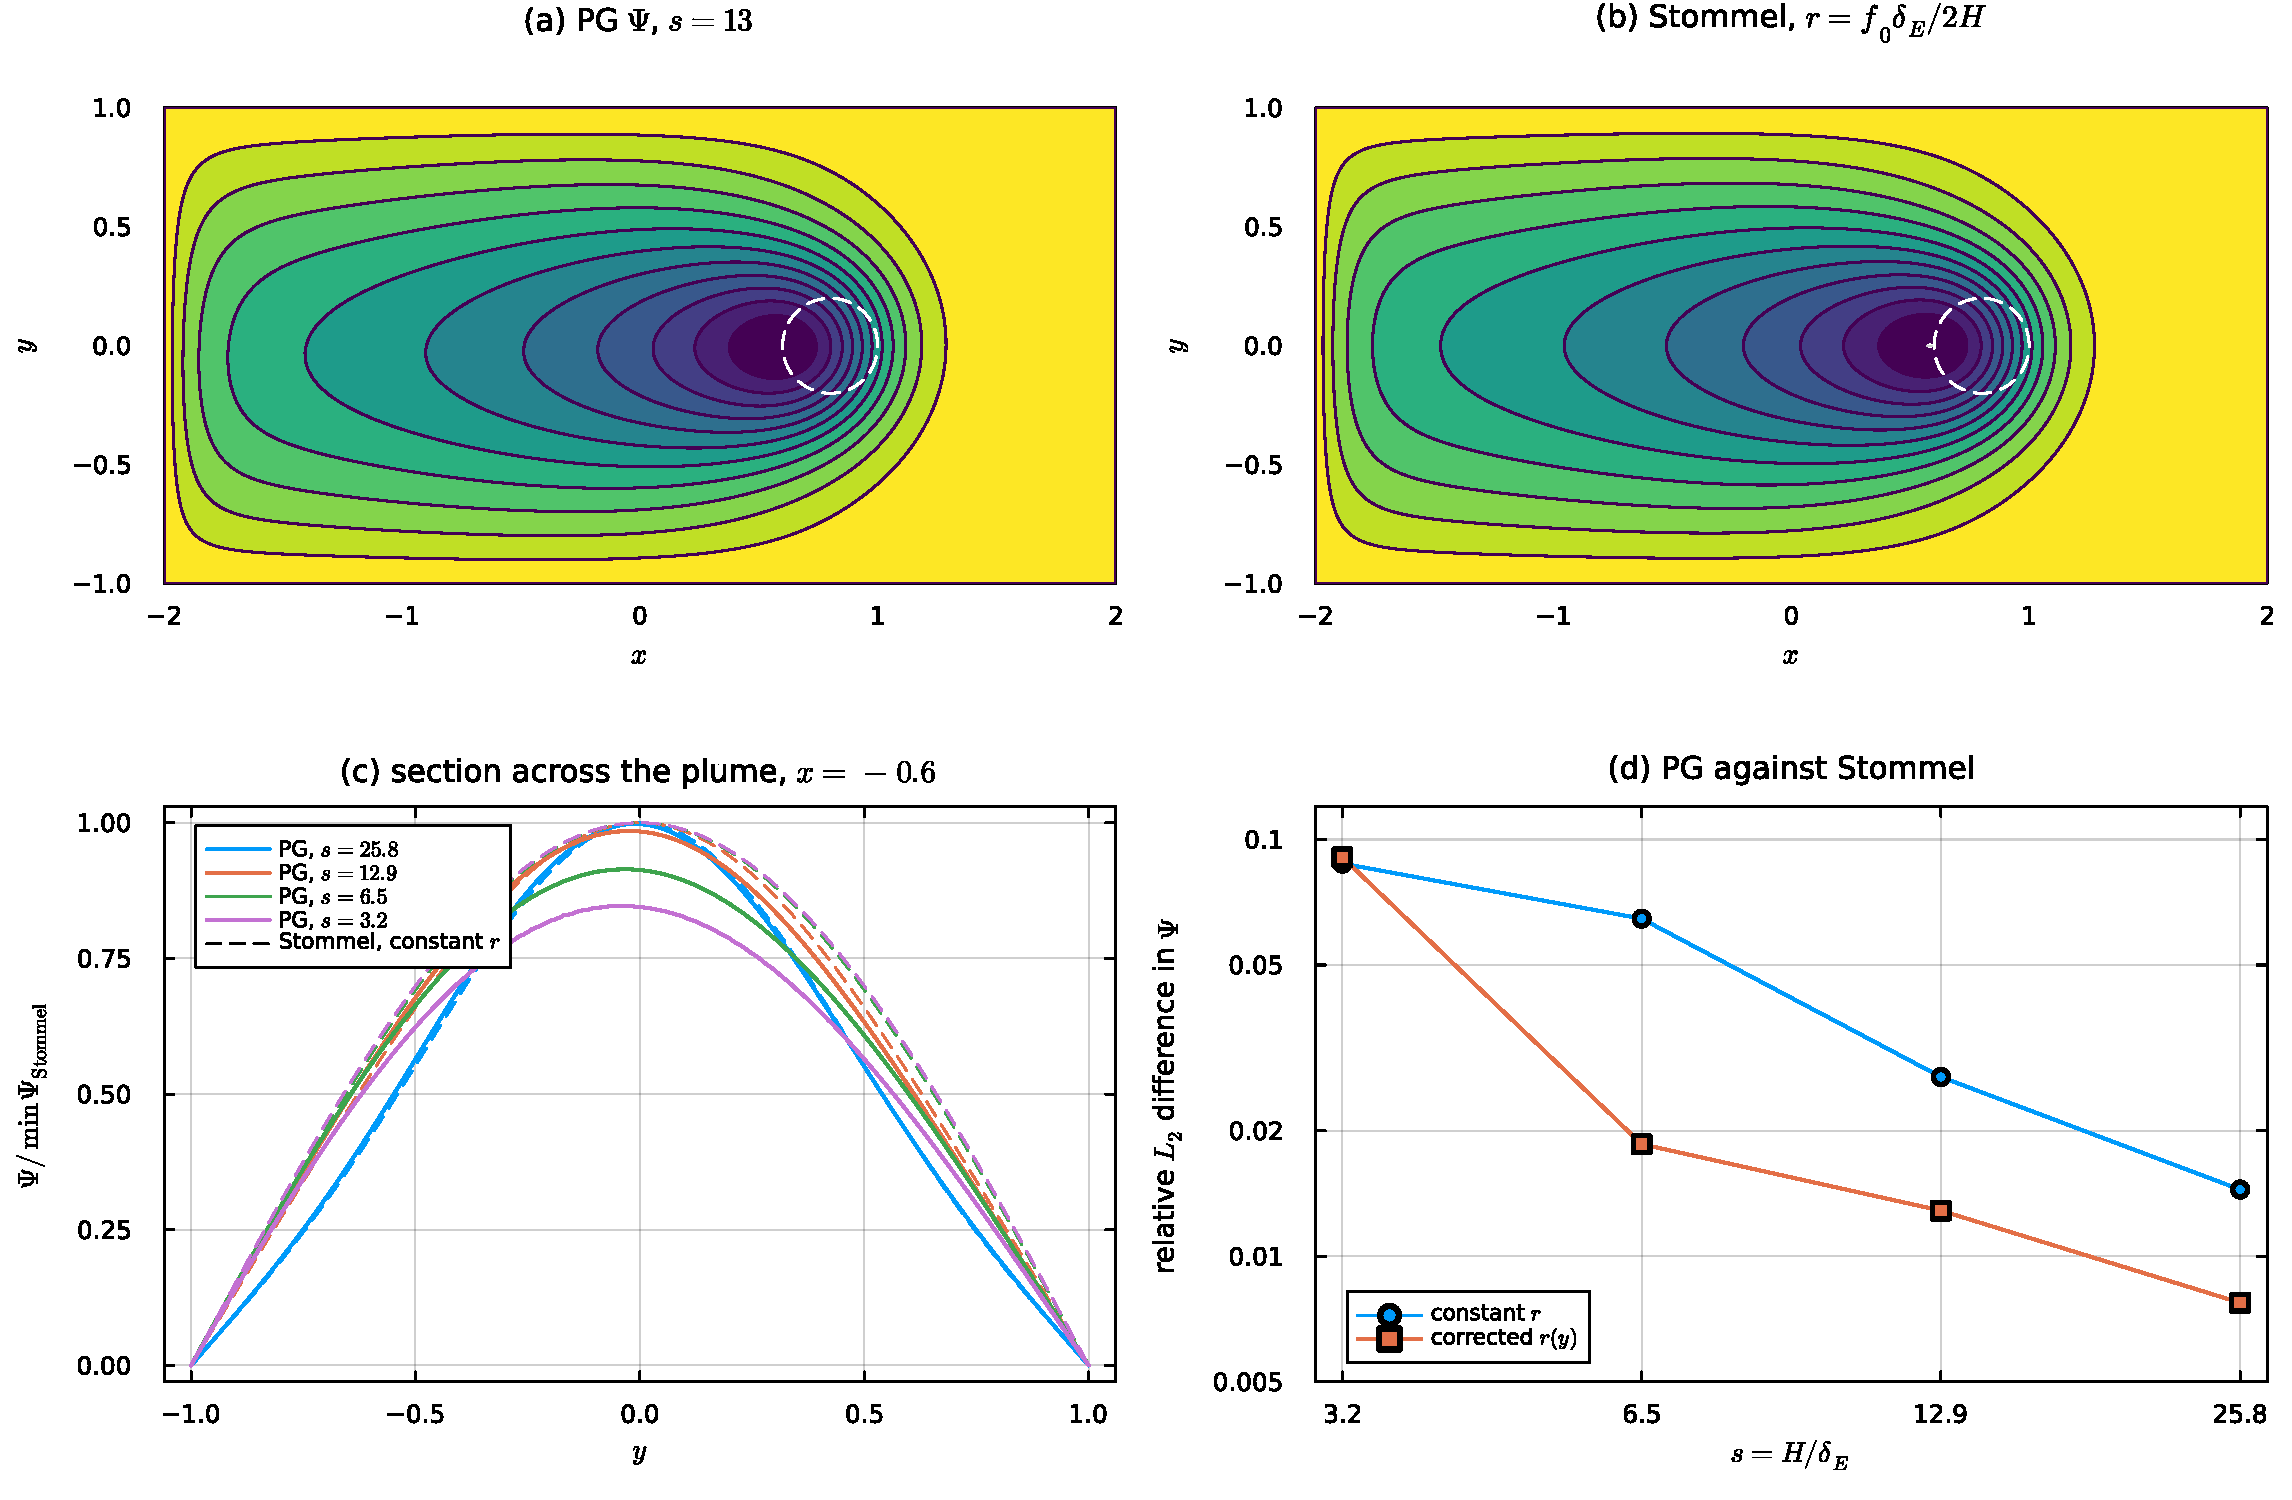
\includegraphics[width=14cm]{beta_plume_comparison.pdf}
\caption{\added[id=CL]{\label{fig:beta_plume_comparison} The $\beta$ plume of \citet{stommel82}.
(a) PG streamfunction $\Psi$ for $s = H/\delta_E = 13$ ($\mathrm{Ek} = 3 \times 10^{-3}$), with the forcing patch dashed, and (b) the classical frictional solution with the derived drag $r = f_0 \delta_E/(2H)$, on the same contour levels.
(c) Meridional sections of $\Psi$ across the plume at $x = -0.6$ for four values of $s$: PG (solid) and the classical solution (dashed), normalized by the classical extremum.
(d) Relative $L_2$ difference between the PG and classical $\Psi$ against $s$, for the constant drag and for the local drag $r(y) = f \delta_E/[2(H - \delta_E/2)]$.}}
\end{figure}

\begin{figure}
\centering
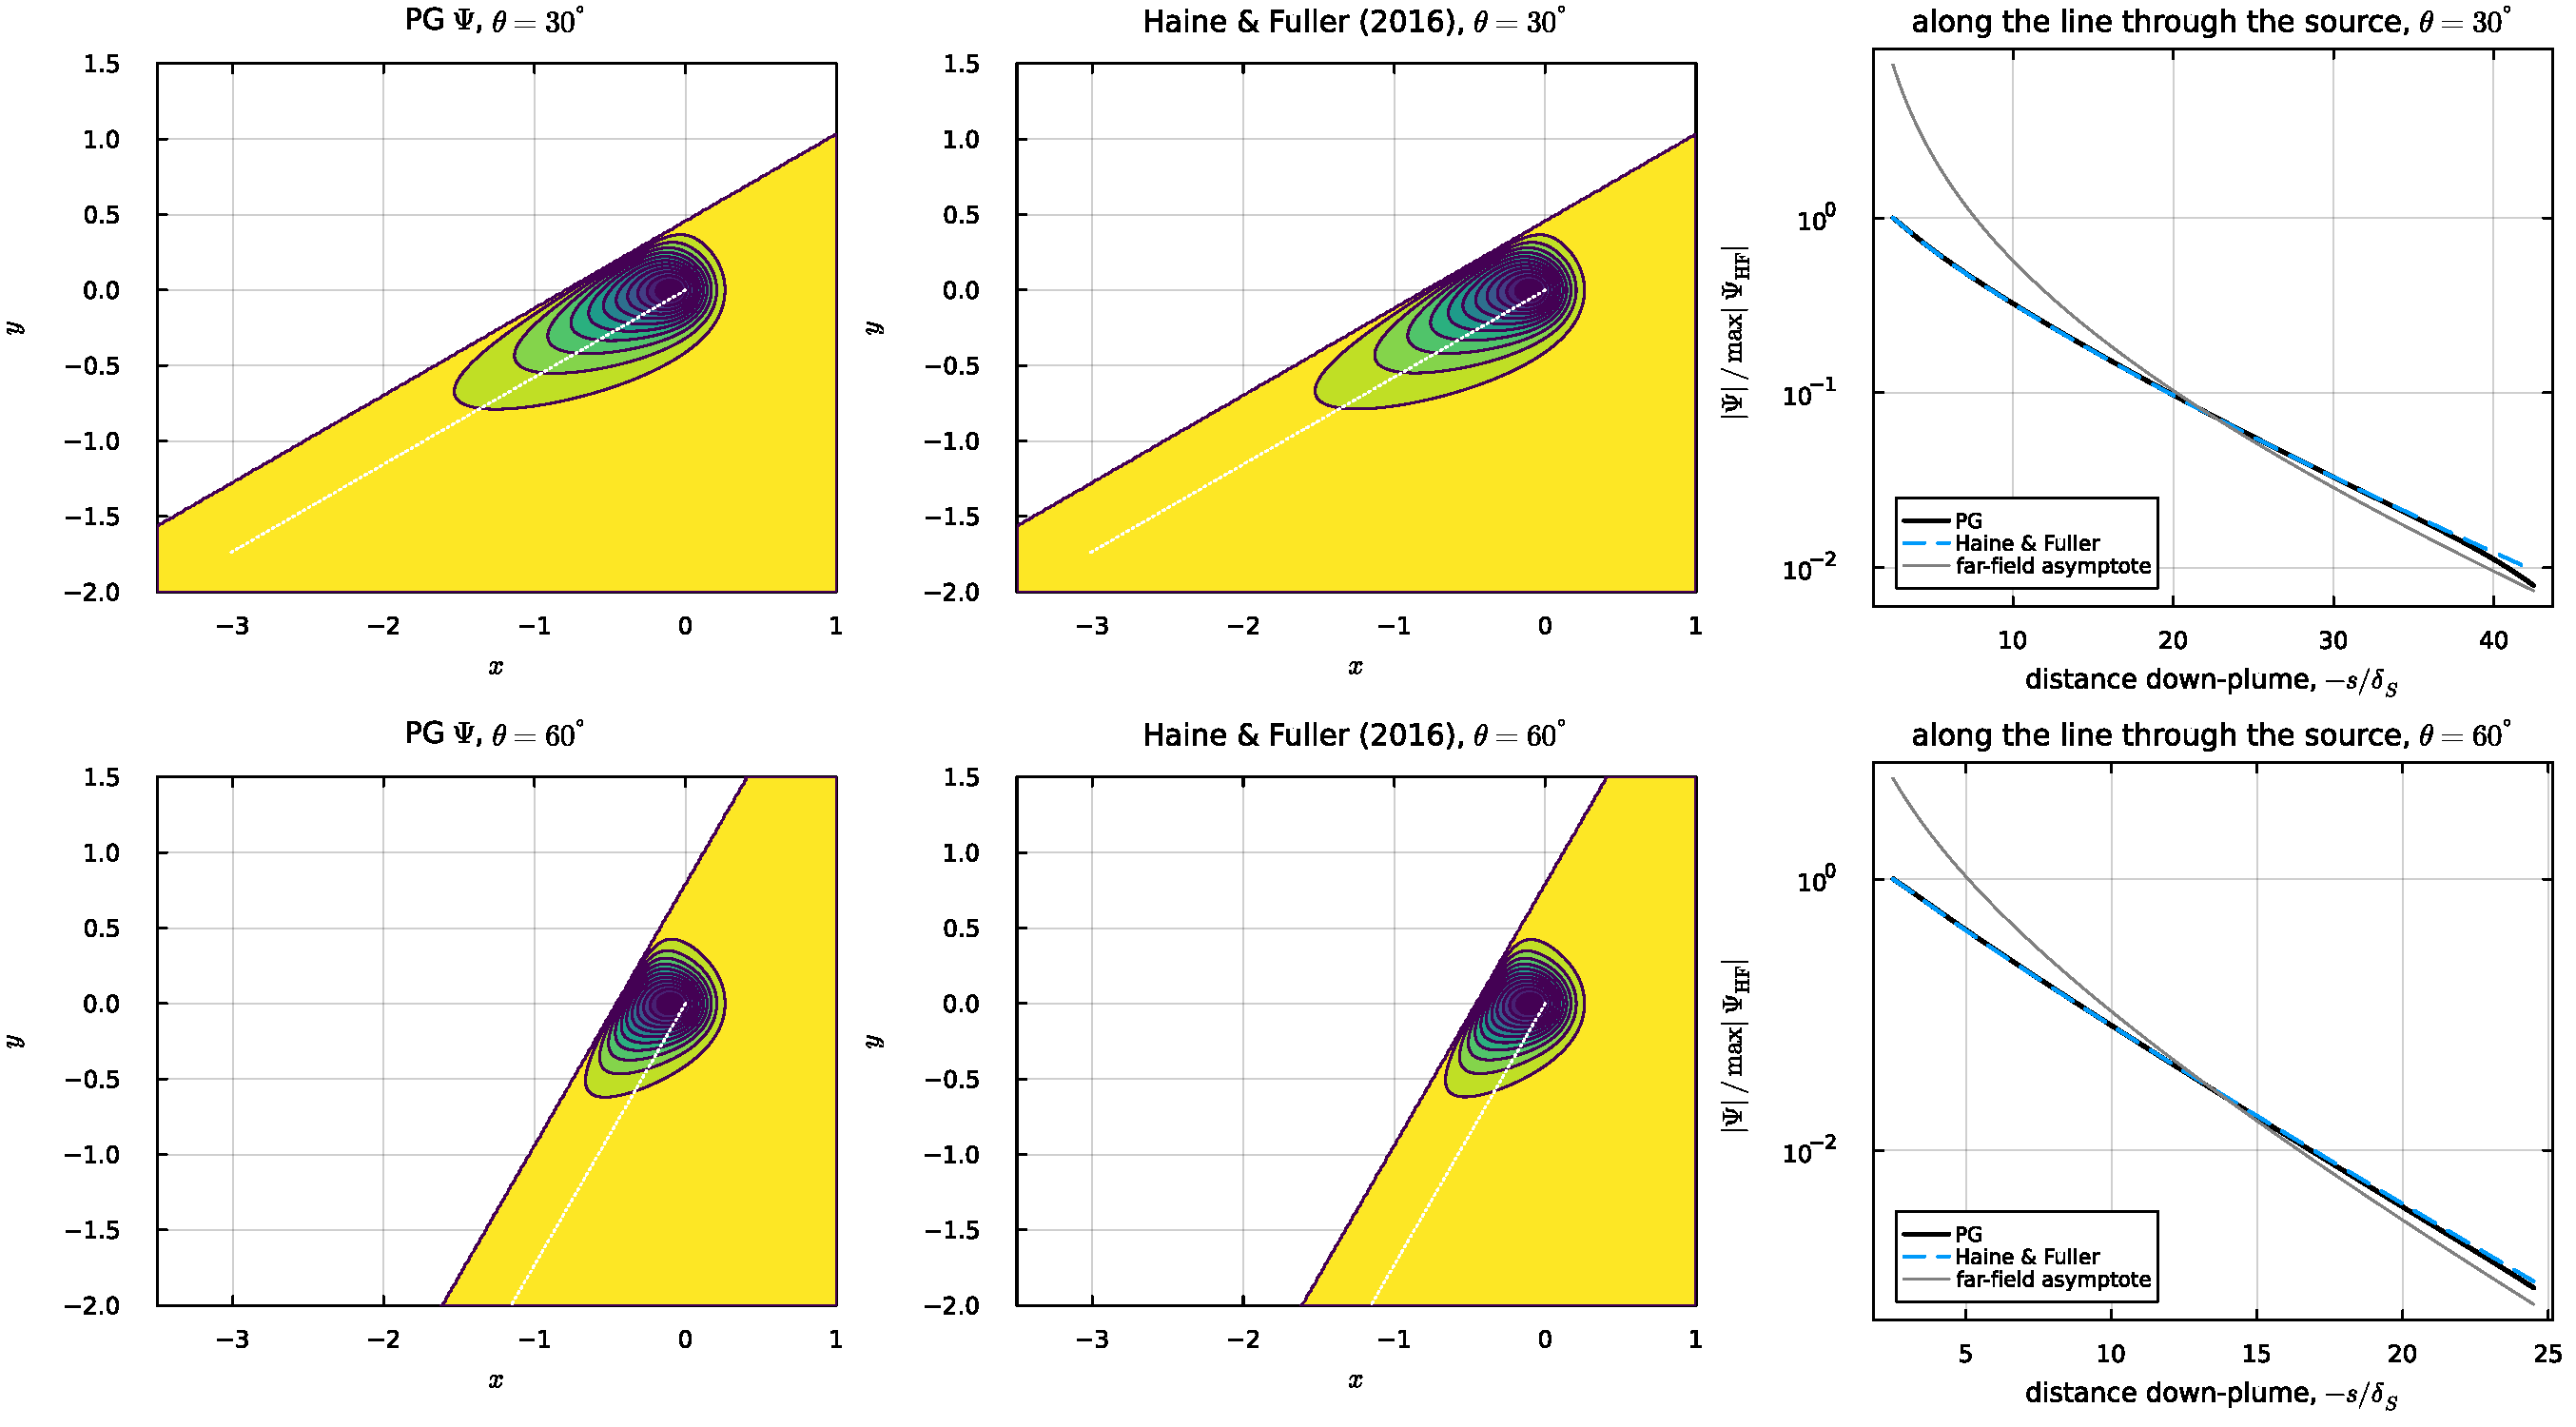
\includegraphics[width=16cm]{boundary_beta_plume_comparison.pdf}
\caption{\added[id=CL]{\label{fig:boundary_beta_plume_comparison} Boundary $\beta$ plumes of \citet{haine&fuller16}, for a coast inclined at $\theta = 30^\circ$ (top) and $60^\circ$ (bottom) to east--west.
Left: PG streamfunction $\Psi$. Centre: the exact solution of \citet{haine&fuller16} with the derived drag $\lambda = f_0 \delta_E/(2H)$, convolved with the Gaussian source, on the same contour levels. The dotted line runs through the source parallel to the coast.
Right: $|\Psi|$ along that line against down-plume distance in units of $\delta_S = \lambda/\beta$, for PG (solid), the exact solution (dashed), and the far-field asymptote }\added[id=CL]{$\propto d^{-3/2} \exp[-d(1 - \cos \theta)/2\delta_S]$, with $d$ the down-plume distance}\added[id=CL]{ (gray).}}
\end{figure}

\paragraph{\added[id=CL]{Topographic steering.}}
\added[id=CL]{On an $f$-plane, a shelf of depth 0.1 in the north of a $4 \times 2$ basin falls across a slope, $H = 0.1 + 0.45 \left[ 1 - \tanh \left( (y - 0.3)/0.25 \right) \right]$, to depth 1 in the south.
An isolated patch of wind-stress curl on the slope drives a topographic $\beta$ plume that runs west along the isobaths, with shallow water to the right.
The classical layer model is the deep limit of the PG transport (Section~\ref{sect:results}a): geostrophic transport over a depth $H_g$ plus the bottom Ekman transport down the surface-pressure gradient, $f (\mathbf{U} - \mathbf{U}_E) = -(\delta_E/2) \nabla p_s + H_g \, \hat{\mathbf{z}} \times \nabla p_s$, with $\mathbf{U}_E$ the surface Ekman transport.
Eliminating $p_s$ gives an elliptic equation for $\Psi$ that, for $\delta_E \ll H_g$, steers $\Psi$ along contours of $f/H_g$ with drag $f \delta_E/(2 H_g^2)$; it is solved by finite differences in the same basin.
With classical $f/H$ steering ($H_g = H$), the relative $L_2$ difference in $\Psi$ over the deep basin ($H > 0.6$) is 15\%, 4.3\%, and 2.0\% for $\mathrm{Ek} = 5 \times 10^{-3}$, $1.25 \times 10^{-3}$, and $2 \times 10^{-4}$, where the deep basin has $s = 10$, 20, and 50.
Steering along $f/(H - \delta_E/2)$ ($H_g = H - \delta_E/2$), with the bottom Ekman layer as a displacement thickness, reduces it to 6.2\%, 2.0\%, and 0.2\% (Fig.~\ref{fig:topographic_steering_comparison}).
On the shelf ($H < 0.2$), where $s = 1$, 2, and 5, the differences are 52\%, 13\%, and 4.4\% with $f/H$ steering, and 40\%, 13\%, and 0.6\% with $f/(H - \delta_E/2)$.
Where the shelf is less than about two Ekman depths deep, the Ekman layers overlap, the transport becomes the lubrication flow down the pressure gradient of Section~\ref{sect:results}a, and neither steering depth recovers the PG solution.}

\begin{figure}
\centering
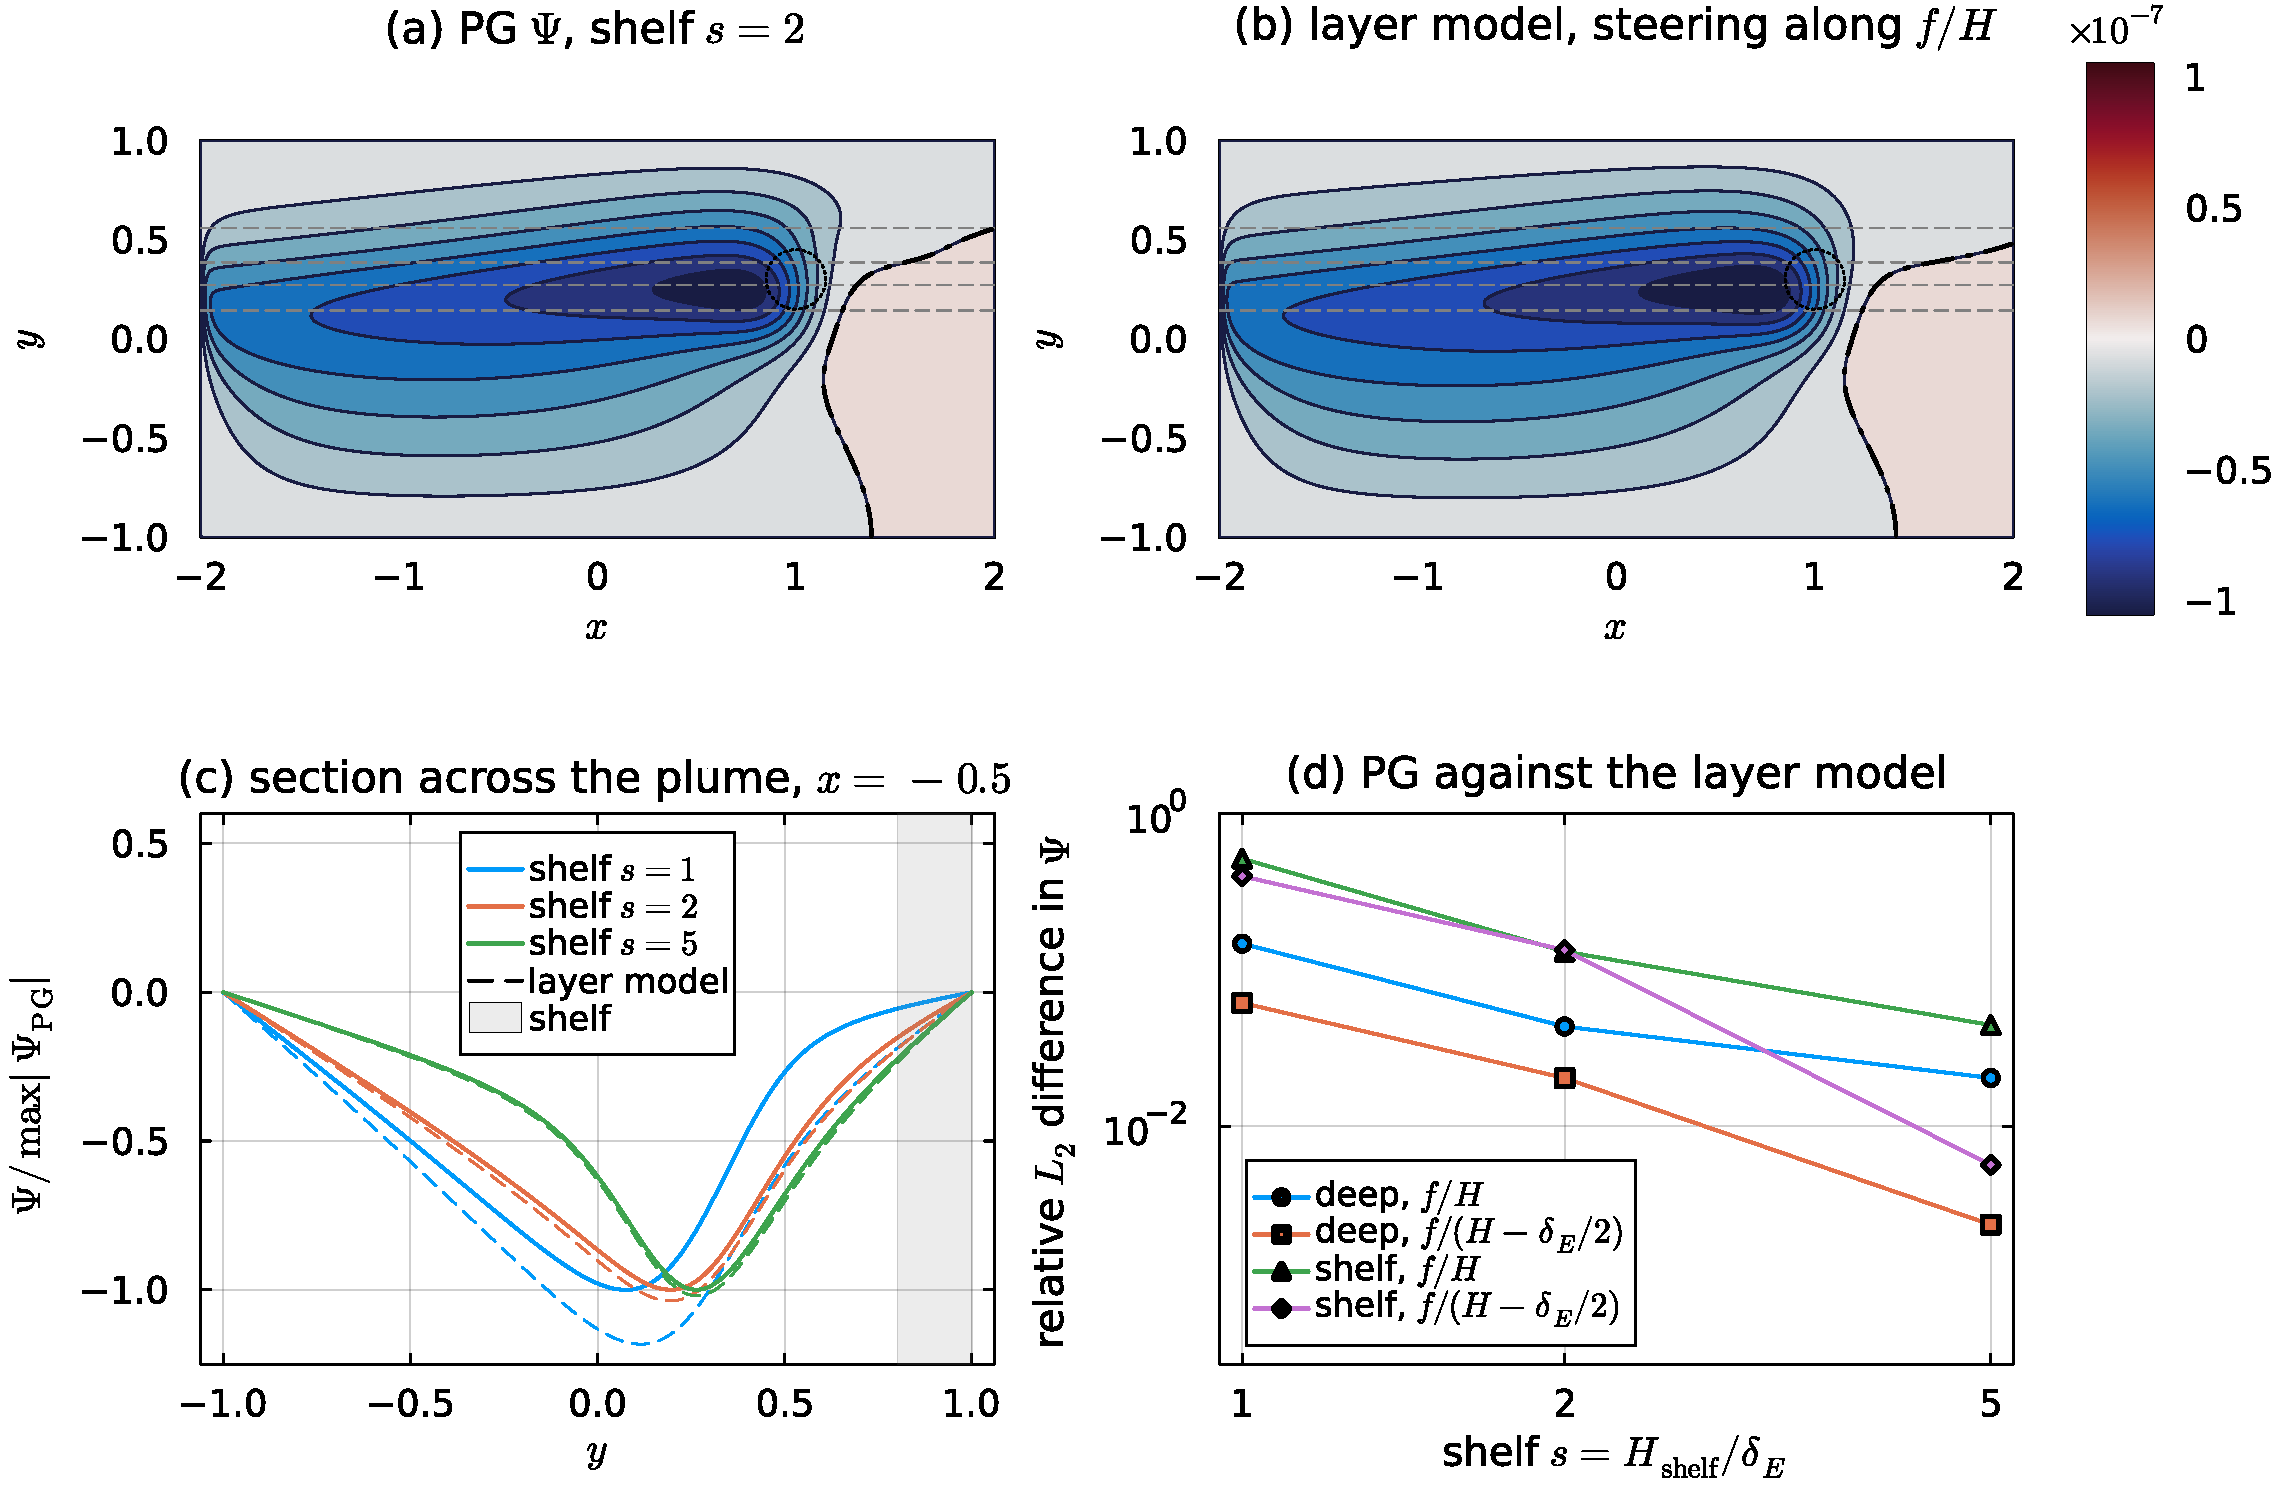
\includegraphics[width=14cm]{topographic_steering_comparison.pdf}
\caption{\added[id=CL]{\label{fig:topographic_steering_comparison} Topographic steering over a slope to a shallow shelf, on an $f$-plane.
(a) PG streamfunction $\Psi$ for $\mathrm{Ek} = 1.25 \times 10^{-3}$ (shelf $s = 2$, deep $s = 20$), and (b) the layer model with steering along $f/H$, on the same contour levels. Gray dashed lines are isobaths $H = 0.2$, 0.4, 0.6, and 0.8, the black dash-dotted line is $\Psi = 0$, and the dotted circle marks the forcing patch.
(c) Meridional sections of $\Psi$ at $x = -0.5$ for shelf $s = 1$, 2, and 5: PG (solid) and the layer model with $f/H$ steering (dashed), normalized by the PG extremum; the shaded band is the shelf.
(d) Relative $L_2$ difference between the PG and layer-model $\Psi$ over the deep basin ($H > 0.6$) and the shelf ($H < 0.2$), with steering along $f/H$ and along $f/(H - \delta_E/2)$, against the shelf $s$.}}
\end{figure}

% Added by Claude (CL): Section 6d, double-basin showcase. Made by TheoryNotes/DoubleBasinShowcase.jl.
\subsection{A double basin}
\label{sect:double_basin}

\added[id=CL]{To show the method on a less idealized geometry, Fig.~\ref{fig:double_basin_showcase} shows a double basin on an $f$-plane with $\mathrm{Ek} = 0.002$, so that $\delta_E = 0.063$.
Two deep bowls are separated by a shallow ridge running west from the eastern shelf and joined by a deeper western strait, loosely modeled on the Nordic Seas and Fram Strait.
The outer shelf is 0.26 deep, only 4.1 Ekman depths}\added[id=CL]{, close to the depth below which the Ekman layers begin to overlap (Section~\ref{sect:results}a),}\added[id=CL]{ and the deepest water is about 19 Ekman depths.
Cyclonic wind-stress cells over each bowl, a meridional surface-buoyancy gradient, and uniform restoring stratification drive the circulation.
The steady circulation consists of two cyclonic gyres steered by the closed isobaths of each bowl, joined through the strait, where the meridional velocity is nearly uniform with depth down to the bed (Fig.~\ref{fig:double_basin_showcase}a, b).}

\added[id=CL]{Table~\ref{tab:double_basin} lists the cost of each stage on 18 threads.
The solve on a mesh of size 0.02 takes 8~s, }\replaced[id=CR]{and the depth-integrated momentum balance and the three independent vorticity balances (BV, GCVB, and TDVB) take a further 17~s on a $65 \times 65$ diagnostic grid.}{and all five dynamical balances of Table~\ref{tab:dynamical_balances} take a further 19~s on a $65 \times 65$ diagnostic grid.}\added[id=CL]{
The depth-integrated momentum balance closes to $10^{-5}$, and the cell-averaged vorticity balances to 3\%, the residual being set by the diagnostic grid (Section~\ref{sect:results}\ref{sect:verification}).}

\added[id=CL]{The solution also tests the integral constraint of \citet{nost&isachsen03}.
On closed $f/H$ contours, the bottom geostrophic velocity follows from the forcing integrated over the enclosed area once a drag law is assumed.
With a linear or quadratic isotropic drag, calibrated by least squares against the PG bottom stress itself, the predicted bottom velocity differs from the PG velocity by 103\% and 120\% (relative $L_2$, 2771 points), although the speeds remain correlated (0.92 and 0.88).
With the drag derived from the PG bottom stress, }\added[id=CL]{$\tau_b^x + i \tau_b^y = S (\partial_x + i \partial_y) p_s + T$ (\ref{eqn:bottom_stress_ST_def})}\added[id=CL]{, which is rotated relative to the bottom velocity and includes the baroclinic and wind contributions, the same constraint reproduces the PG bottom velocity to 3\% (Fig.~\ref{fig:double_basin_showcase}c).
The drag closure, not the integral constraint, limits the classical method.}

\added[id=CL]{Finally, one adjoint solve of the surface-pressure equation gives the sensitivity of the northward transport through the strait to the wind stress, surface buoyancy, and restoring buoyancy everywhere (Fig.~\ref{fig:double_basin_showcase}d--f).
The adjoint identity holds to $10^{-14}$, }\added[id=CL]{and the adjoint solve and kernel sampling take 21~s.}\added[id=CL]{
The kernels extend from the strait along the isobaths of the western slope and around the southern bowl, mapping the region whose forcing sets the strait transport.}

\begin{table}
\caption{\added[id=CL]{\label{tab:double_basin} Wall-clock times on 18 threads (Apple M5 Max) for the double basin of Fig.~\ref{fig:double_basin_showcase}, and the closure of each balance as the relative $L_2$ residual on the $65 \times 65$ diagnostic grid.}\added[id=CR]{ The DIV balance is identical to the BV balance (Section~\ref{sect:dynamical_balances}) and is not listed.}}
\centering
\begin{tabular}{lcc}
\hline
Stage & Time (s) & Residual \\
\hline
PG solve, mesh 0.02 (153\,876 quadrature points) & 7.7 & \\
3-D sampling, $241 \times 3 \times 121$ points & 1.6 & \\
Transport, bottom stress, and $\Psi$ & 5.6 & \\
Depth-integrated momentum (DIM) & 0.6 & $1.0 \times 10^{-5}$ \\
Barotropic vorticity (BV), cell averages & 13.2 & 0.034 \\
\deleted[id=CR]{Depth-integrated vorticity (DIV)} & \deleted[id=CR]{2.0} & \deleted[id=CR]{0.034} \\
Geostrophic-contour vorticity (GCVB) & 1.6 & 0.027 \\
Transport-divergence vorticity (TDVB) & 1.6 & 0.034 \\
Nøst--Isachsen comparison & 1.6 & \\
Adjoint sensitivity of the strait transport & 21.1 & \\
\hline
\end{tabular}
\end{table}

\begin{figure}
\centering
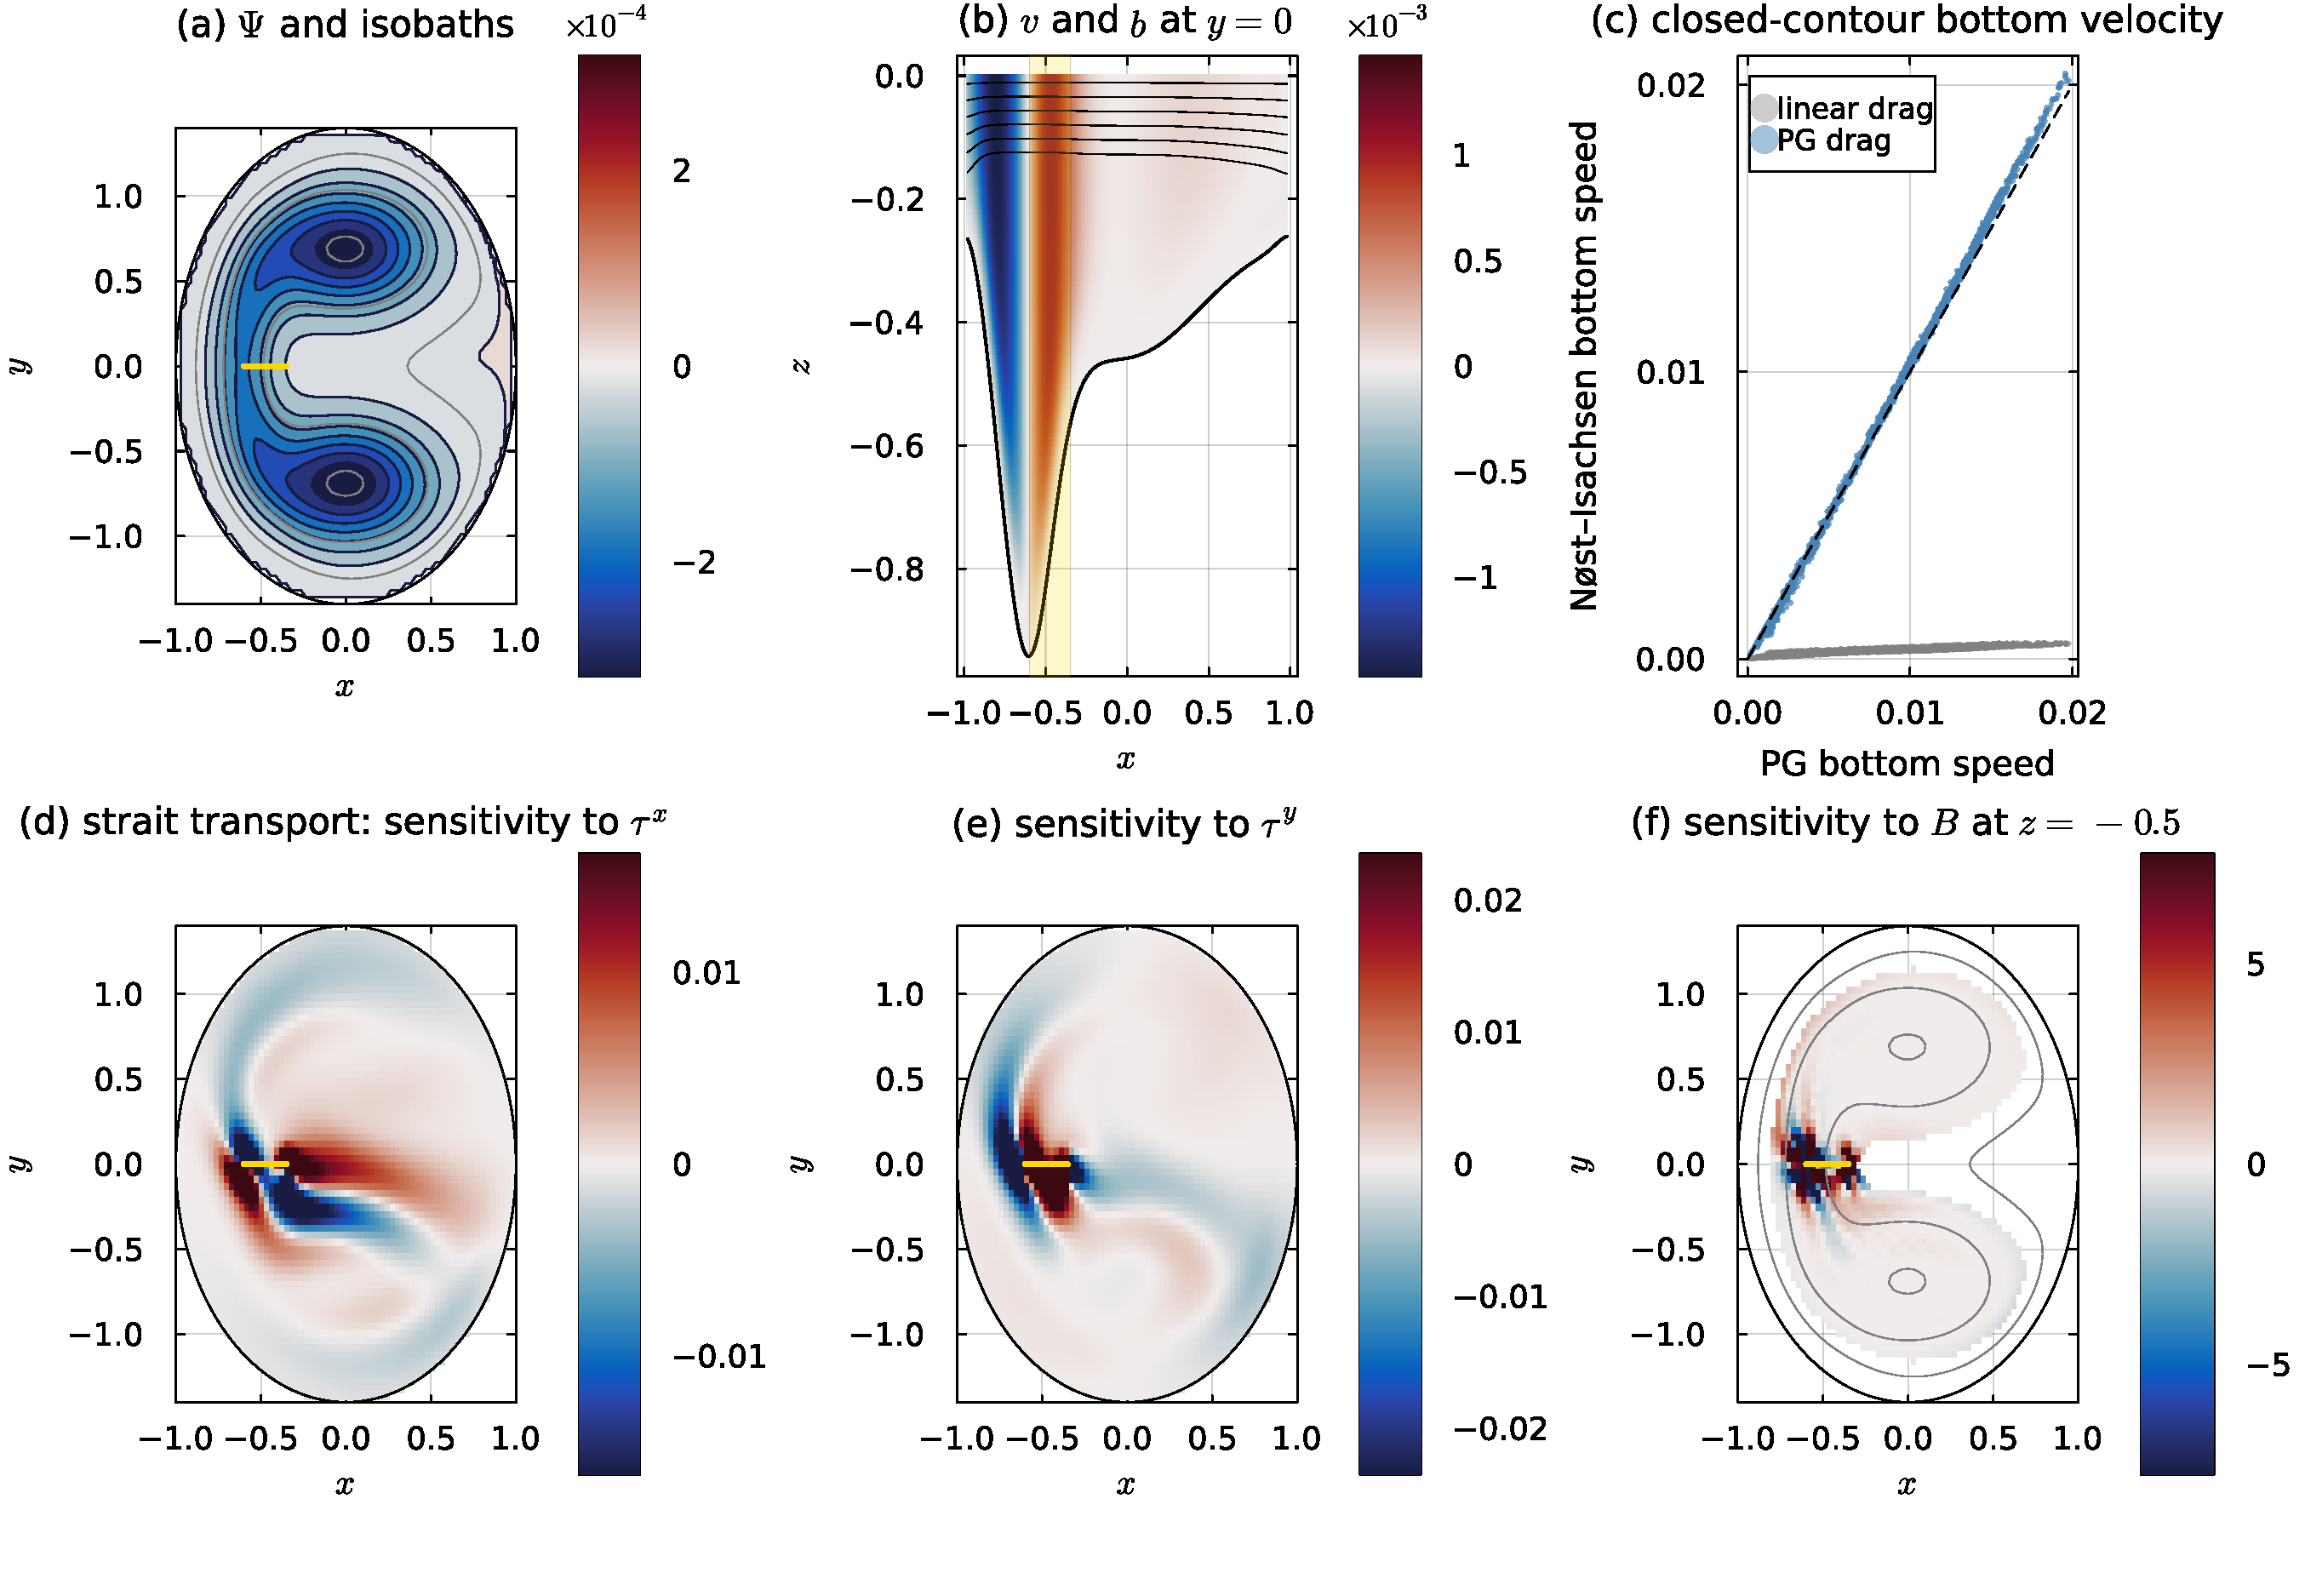
\includegraphics[width=16cm]{double_basin_showcase.pdf}
\caption{\added[id=CL]{\label{fig:double_basin_showcase} Double basin on an $f$-plane, $\mathrm{Ek} = 0.002$.
(a) Transport streamfunction $\Psi$, with isobaths $H = 0.4$, 0.8, and 1.2 (gray) and the strait section (gold).
(b) Meridional velocity $v$ (color) and buoyancy $b$ (contours) in a zonal section at $y = 0$; the strait section is shaded.
(c) Bottom speed on closed $f/H$ contours from the \citet{nost&isachsen03} integral constraint against the PG bottom speed, with an assumed linear drag calibrated against the PG bottom stress (gray) and with the drag derived from the PG bottom stress (blue); percentages are relative $L_2$ velocity differences.
(d--f) Adjoint sensitivity of the northward strait transport to the local wind stress $\tau^x$ and $\tau^y$, and to the restoring buoyancy $B$ at $z = -0.5$; color scales are clipped at the 97th percentile of the magnitude.}}
\end{figure}

% Added by Claude (CL): Section 6e, cost and dimensional parameters. Made by TheoryNotes/CostScaling.jl.
\subsection{Cost and dimensional parameters}
\label{sect:cost}

\added[id=CL]{Table~\ref{tab:cost_scaling} shows how the wall-clock time cost of the solve scales, in the test basin of Section~\ref{sect:results}\ref{sect:verification} on 18 threads.
The evaluation of the column integrals for $\mathfrak{A}$, $\mathfrak{B}$, $S$, and $T$ at the quadrature points of the }\added[id=CL]{surface-pressure mesh dominates the time cost}\added[id=CL]{; the finite-element assembly and linear solve take at most a fifth.
At fixed $\mathrm{Ek}$, the cost is proportional to the number of quadrature points, from 0.22~s at $h = 0.08$ to 11.7~s at $h = 0.01$.
At fixed mesh, it grows with $s = H/\delta_E$, because each column is split into $\lceil H/(4\delta_E) \rceil$ Gauss--Legendre panels: from 0.75~s at $\mathrm{Ek} = 10^{-2}$ to 202~s at $\mathrm{Ek} = 10^{-5}$, faster than $s$.
The column integrals are independent, and the solve at $h = 0.02$ takes 16.9~s on one thread and 2.0~s on 18, a speed-up of 8.5 on a processor with 6 performance and 12 efficiency cores.}

\added[id=CL]{Table~\ref{tab:dimensional} gives dimensional values for a basin of width $L = 1000$~km and depth $H_0 = 4000$~m with $f_0 = 10^{-4}$~s$^{-1}$.
The Ekman numbers of the examples, $0.02$ to $1.3 \times 10^{-4}$, correspond to vertical viscosities of 32 to 0.2~m$^2$\,s$^{-1}$ and Ekman depths of 800 to 64~m.
A realistic $\nu_0 \approx 10^{-2}$~m$^2$\,s$^{-1}$ gives $\mathrm{Ek} \approx 6 \times 10^{-6}$ and $\delta_E \approx 14$~m.
Two costs limit such small Ekman numbers.
The column integrals grow with $s$, which reaches about 300, and the mesh must resolve the frictional layers of width $\ell \approx \delta_E/(2|\nabla H|)$ over slopes (Section~\ref{sect:results}\ref{sect:classical_limits})}\added[id=CL]{, about 0.1--1~km for continental slopes with $|\nabla H| \approx 0.01$--0.05 and a few kilometers only for gentle slopes of $10^{-3}$.}\added[id=CL]{
Extrapolating linearly from $\mathrm{Ek} = 10^{-5}$ at $h = 0.04$, }\added[id=CL]{a uniform mesh of size $h = 0.005$ (5~km), fine enough only for gentle slopes, would take about 4~hours on 18 threads, and resolving continental slopes with a uniform mesh would cost $10^2$ to $10^4$ times more, which is impractical, so realistic Ekman numbers call for meshes refined over steep slopes.}\added[id=CL]{}

\begin{table}
\caption{\added[id=CL]{\label{tab:cost_scaling} Wall-clock time of the PG solve (best of three, after compilation) in the test basin of Section~\ref{sect:results}\ref{sect:verification}, on 18 threads of an Apple M5 Max unless stated. The forcing evaluation computes the column integrals at the quadrature points of the surface-pressure mesh. The script is \texttt{TheoryNotes/CostScaling.jl}.}}
\centering
\begin{tabular}{lrrrr}
\hline
Case & Quadrature points & Total (s) & Forcing (s) & Assembly and solve (s) \\
\hline
$\mathrm{Ek} = 10^{-2}$, $h = 0.08$ & 5\,988 & 0.22 & 0.18 & 0.01 \\
$\mathrm{Ek} = 10^{-2}$, $h = 0.04$ & 21\,576 & 0.76 & 0.65 & 0.04 \\
$\mathrm{Ek} = 10^{-2}$, $h = 0.02$ & 82\,896 & 2.58 & 2.16 & 0.22 \\
$\mathrm{Ek} = 10^{-2}$, $h = 0.01$ & 328\,152 & 11.7 & 8.93 & 2.15 \\
\hline
$\mathrm{Ek} = 10^{-3}$, $h = 0.04$ ($s \le 31$) & 21\,576 & 3.35 & 3.24 & 0.04 \\
$\mathrm{Ek} = 10^{-4}$, $h = 0.04$ ($s \le 99$) & 21\,576 & 22.3 & 22.2 & 0.05 \\
$\mathrm{Ek} = 10^{-5}$, $h = 0.04$ ($s \le 313$) & 21\,576 & 202 & 202 & 0.04 \\
\hline
$\mathrm{Ek} = 10^{-2}$, $h = 0.02$, 1 thread & 82\,896 & 16.9 & 16.6 & 0.21 \\
\quad 2 / 4 / 8 / 18 threads & & 10.5 / 5.0 / 3.4 / 2.0 & & \\
\hline
\end{tabular}
\end{table}

\begin{table}
\caption{\added[id=CL]{\label{tab:dimensional} Dimensional values for $L = 1000$~km, $H_0 = 4000$~m, $f_0 = 10^{-4}$~s$^{-1}$, and $\nu = \kappa$ ($\mathrm{Pr} = 1$): $\nu_0 = \mathrm{Ek}\, f_0 H_0^2$ and $\delta_E = H_0 \sqrt{2\,\mathrm{Ek}}$.
The nondimensional $\beta = 0.15$ of the test basin is $1.5 \times 10^{-11}$~m$^{-1}$\,s$^{-1}$, and $\Gamma = 0.2$ is a relaxation rate $\gamma = \Gamma f_0/\mathrm{Pr} = 2 \times 10^{-5}$~s$^{-1}$ (0.6~days).}}
\centering
\begin{tabular}{lccc}
\hline
Example & $\mathrm{Ek}$ & $\nu_0$ (m$^2$\,s$^{-1}$) & $\delta_E$ (m) \\
\hline
\texttt{Oceananigans.jl} comparison (Appendix C) & 0.02 & 32 & 800 \\
Test basin (Section~\ref{sect:results}\ref{sect:verification}) & 0.01 & 16 & 570 \\
Double basin (Section~\ref{sect:results}\ref{sect:double_basin}) & 0.002 & 3.2 & 250 \\
Boundary $\beta$ plume (Section~\ref{sect:results}\ref{sect:classical_limits}) & $1.3 \times 10^{-4}$ & 0.20 & 64 \\
Realistic & $6 \times 10^{-6}$ & 0.01 & 14 \\
\hline
\end{tabular}
\end{table}

\section{Discussion}
\label{sect:discussion}

% Added by Claude (CL): Discussion drafted from the original bullet list.
\added[id=CL]{The linear robust-diagnostic PG equations have been solved exactly for an arbitrary basin, bathymetry, and Coriolis parameter, with the surface and bottom Ekman layers resolved even where they overlap.
The three-dimensional problem reduces to closed-form Green's functions in each column and one two-dimensional advection--diffusion equation for the surface pressure, whose coefficients $\mathfrak{A}$ and $\mathfrak{B}$ are exact column integrals.
The solution has been verified against independent implementations of the column solution, under mesh refinement, by closure of every depth-integrated balance, and against a primitive-equation model, and it takes seconds to compute }\added[id=CL]{(Sections~\ref{sect:results}\ref{sect:verification} and \ref{sect:results}\ref{sect:cost})}\added[id=CL]{.
Because the solution is exact, the depth-integrated momentum and vorticity balances, the integral constraints on closed contours, and the sensitivities to the forcing can all be evaluated without a parameterized drag or a residual of unknown origin.}

\added[id=CL]{The exact coefficients also sharpen several classical rules of thumb }\added[id=CL]{(Sections~\ref{sect:results}a and \ref{sect:results}\ref{sect:classical_limits})}\added[id=CL]{.
First, the depth-integrated flow is steered along contours of $f/(H - \delta_E/2)$ rather than $f/H$, because the bottom Ekman layer acts as a displacement thickness; in the topographic steering test this correction reduces the error of the layer model from 2\% to 0.2\% at $s = H/\delta_E = 50$.
Second, the bottom drag is not a free parameter: in deep water it is the linear drag $f \delta_E/(2H)$ of \citet{stommel48}, rotated by $45^\circ$, and it varies with latitude as $f^{1/2}$, which accounts for much of the difference between the PG solutions and the classical Stommel gyre and $\beta$ plume.
Third, a single length, $\ell = |\mathfrak{A}^r| / |\nabla \mathfrak{A}^i| \approx \delta_E / \left[ 2 f \left| \nabla (H/f) \right| \right]$ for deep water $H \gg \delta_E$, namely, the ratio of the frictional diffusivity to the steering speed in the surface-pressure equation (\ref{eqn:ps}), sets the width of the frictional layer where the steering flow meets a coast.
The $\ell$ formula yields Stommel's lengthscale $r/\beta$ on a flat $\beta$-plane, with $r = f \delta_E/(2H)$ the linear drag coefficient of Section~\ref{sect:results}a, and $\delta_E/(2|\nabla H|)$ over a slope.
Along coasts parallel to the steering flow, frictional layers instead widen as $\sqrt{\ell d}$ with along-coast distance $d$.
Fourth, the classical layer picture holds where the water is deeper than about three Ekman depths; }\added[id=CL]{where it is shallower than one to two,}\added[id=CL]{ the Ekman layers overlap, the transport becomes a lubrication flow down the pressure gradient, and $f/H$ contours no longer guide it.
The double basin shows the practical consequence: the integral constraint of \citet{nost&isachsen03} reproduces the bottom velocity on closed $f/H$ contours to 3\% with the derived bottom stress, }\added[id=CL]{but errs by more than 100\% with an isotropic drag}\added[id=CL]{ calibrated against the same stress (Section~\ref{sect:results}\ref{sect:double_basin}).}

\added[id=CL]{The solution has limitations, each of which involves some excluded physics.
Buoyancy is not advected, so the density field is prescribed through the restoring field $B$ and the surface buoyancy $b_s$.
Robust-diagnostic PG therefore cannot produce a $\beta$ spiral \citep{schott&stommel78}, for example.
Friction is vertical only, so the frictional boundary layers are of Stommel type, and the viscous sublayers of \citet{munk50} are absent; in the comparison with \texttt{Oceananigans.jl}, it was the $z$-level model that needed horizontal viscosity to suppress grid-scale noise over a sloping bottom (Appendix~C).}
\added[id=CL]{The viscosity and diffusivity are uniform in the vertical.
Each column then has a buoyancy bottom boundary layer of thickness $(\kappa\,\mathrm{Ek}/\Gamma)^{1/2}$ in which the no-flux condition $\partial_z b = 0$ bends isopycnals into a sloping bottom, so the solution contains cross-slope buoyancy gradients and a thermal wind near the bed, but not the stronger ones that bottom-enhanced mixing produces as it erodes the stratification \citep{peterson&callies23,peterson&callies26}.
Such diffusivity profiles, like the exponential profile of \citet{peterson&callies26}, need new Green's functions; for exponential profiles they can be found using hypergeometric functions (Appendix~A).
As in \citet{peterson&callies26}, the $\delta^2$ term of the full bottom buoyancy condition (\ref{eqn:bot_b_bc}) is dropped; it matters only over slopes steep enough that the normal and vertical directions differ appreciably.}
\added[id=CL]{Finally, the solution is steady, uses a rigid lid in which the surface pressure stands for the surface height, and requires $f \neq 0$, so the deep tropics are excluded.
The cost of small Ekman numbers is discussed in Section~\ref{sect:results}\ref{sect:cost}: realistic values need meshes refined over steep slopes.}

\added[id=CL]{Within these limits the solution has several uses.
It is a fast solver for the steady external mode given a density field, and could provide a dynamically consistent initial state for the spin-up of ocean general circulation models.
Its exact vorticity budgets, evaluated as cell averages, are a baseline against which the budgets of models with momentum advection, time dependence, or horizontal dissipation can be compared.
The adjoint gives, from one solve, the forcing that controls a chosen transport, as in the strait of the double basin, and it could similarly map the sources of topostrophy, the tendency of the flow }\added[id=CL]{to keep shallow water to its right in the Northern Hemisphere}\added[id=CL]{ \citep{merryfield&scott07,holloway08}.
Applied to climatological density and wind-stress fields, the solution would infer the circulation in the spirit of \citet{nost&isachsen03}, but with a derived rather than a fitted drag.
Horizontal friction, in contrast, would couple neighboring columns and so break the column separability on which the method rests.}

\added[id=CL]{The solution is also a step towards the thermocline problem.
With buoyancy advection, (\ref{eqn:b}) can be written as relaxation to an effective field, $\Gamma (B_{\mathrm{eff}} - b)$ with $B_{\mathrm{eff}} = B - (\mathrm{Pr}\,\mathrm{Bu}/\Gamma)\, \mathbf{u} \cdot \nabla b$, so the linear solution could serve as the inner step of an iteration in which $B_{\mathrm{eff}}$ is updated from the previous velocity and buoyancy.
Whether such an iteration converges, and what thermocline structure it selects, is left for future work.}


%%%%%%%%%%%%%%%%%%%%%%%%%%%%%%%%%%%%%%%%%%%%%%%%%%%%%%%%%%%%%%%%%%%%%
% ACKNOWLEDGMENTS
%%%%%%%%%%%%%%%%%%%%%%%%%%%%%%%%%%%%%%%%%%%%%%%%%%%%%%%%%%%%%%%%%%%%%
\acknowledgments

Tarun Verma and Henry Peterson provided helpful feedback and discussion on the early stages of this work.
Large language models (GPT 5.4 mini, GPT 5.5, GitHub Copliot version 1.1.21, Claude Opus 5.5) were used for assistance with Julia code, especially debugging and plotting of final figures, literature exploration, code generation, and some writing.
The analytical results were supported by the \texttt{SymPy} and \texttt{Symbolics.jl} computer algebra systems \citep{meurer_etal17,gowda_etal21}.

%%%%%%%%%%%%%%%%%%%%%%%%%%%%%%%%%%%%%%%%%%%%%%%%%%%%%%%%%%%%%%%%%%%%%
% DATA AVAILABILITY STATEMENT
%%%%%%%%%%%%%%%%%%%%%%%%%%%%%%%%%%%%%%%%%%%%%%%%%%%%%%%%%%%%%%%%%%%%%
% 
%
\datastatement
All codes to reproduce the analytical and numerical results in this paper are available at \texttt{github.com/ThomasHaine/PlanetaryGeostrophyAnalyticalModel}.
\added[id=CL]{The repository contains the \texttt{PlanetaryGeostrophy} Julia package, which implements the solution, the diagnostics, and the adjoint, with its test suite.
The Jupyter notebooks in \texttt{TheoryNotes/} derive the column solutions with \texttt{SymPy}: \texttt{BuoyancyEquationSolution.ipynb} derives the buoyancy Green's function and its integrals (Section~\ref{sect:b_solution} and Appendix~A; cells 1.1--1.31), and \texttt{FrictionalGeostrophicEquationSolution.ipynb} derives the velocity Green's function, its integrals, the bottom stress, and the coefficients $\mathfrak{A}$, $\mathfrak{B}$, $S$, and $T$ (Section~\ref{sect:PG_soln} and Appendix~B; cells 1.1--1.3 and 2.1--2.7).
\texttt{ComputeQuadratures.ipynb} and \texttt{SymbolicsTesting.jl} build and test the symbolic kernels of Appendix~B.
The figures and tables of Sections~\ref{sect:results}b--e and Appendix~C }\added[id=CL]{are made by the scripts in \texttt{TheoryNotes} and by \texttt{AnalyticalModel/OceananigansComparison.jl}.}\added[id=CL]{}


\section{Appendices}
\appendix[A]
\appendixtitle{Solution to the linear time-independent buoyancy equation}

The problem (\ref{eqn:steady_vertical_b})--(\ref{eqn:simple_bot_b_bc}) is solved as follows using a Green's function $G_b$.
%using a Green's function, , and I suspect also for diffusivity given by an exponential function of depth, as in \citet{peterson&callies26}. 
The Green's function satisfies:
\begin{align}
\partial_ z \left( \kappa \partial_z G_b \right) - \frac{\Gamma }{\mathrm{Ek}} G_b & =  \delta(z - \xi) , \label{eqn:Gsfn}\\
\text{Surface~}z = 0 &: G_b = 0 , \label{eqn:Gsfn_sfcbc} \\
\text{Bottom~}z = -H &: \partial_z G_b = 0 ,
\label{eqn:Gsfn_botbc}
\end{align}
where $\delta(z - \xi)$ is the Dirac delta function.
This is a second order linear ordinary differential equation with two boundary conditions, which can be solved exactly, at least for certain diffusivity profiles.
The solution for uniform non-dimensional diffusivity is
% Notebook cell reference, now summarized in the code-availability statement: (see \texttt{BuoyancyEquationSolution.ipynb} \#1.1, \#1.11)
\begin{align}
G_b (z; \xi) & = \frac{\mathrm{e}^{\psi \left(z + \xi\right)}}
{2 \kappa \psi \left(1 + \mathrm{e}^{2 \psi H}\right)}
\begin{cases} 
\displaystyle \left(1 - \mathrm{e}^{- 2 \psi \xi} \right) \left(\mathrm{e}^{2 \psi H} + \mathrm{e}^{- 2 \psi z  }\right) & \text{for}\: z \leq \xi , \\
\displaystyle \left(1 - \mathrm{e}^{- 2 \psi   z} \right) \left(\mathrm{e}^{2 \psi H} + \mathrm{e}^{- 2 \psi \xi}\right) & \text{for}\: z \geq \xi ,
\end{cases}
% Alternative form: Probably not needed?
% & = \frac{1}
% {2 \kappa \psi \left(1 + \mathrm{e}^{2 \psi H}\right)}
% \begin{cases} 
% \displaystyle \left(1 + \mathrm{e}^{2 \psi (z + H)} \right) \mathrm{e}^{ -\psi z} \left( \mathrm{e}^{\psi \xi} - \mathrm{e}^{-\psi \xi} \right)
% & \text{for}\: z \leq \xi , \\
% \displaystyle 
% \left(\mathrm{e}^{2 \psi z} - 1 \right) \mathrm{e}^{ \psi( 2 H - z)} \mathrm{e}^{\psi \xi}
% + \left(\mathrm{e}^{\psi z } - \mathrm{e}^{-\psi z } \right)  \mathrm{e}^{-\psi \xi}
% & \text{for}\: z \geq \xi ,
% \end{cases}
\end{align}
with $\psi = \sqrt{\Gamma / (\kappa \, \mathrm{Ek}) } $. 
To compute the contribution from the surface buoyancy field $b_s$ to $b$ we need the $\xi$ derivative of the buoyancy Green's function at the surface, which is
\begin{align}
\partial_\xi G_b(z;\xi)|_{\xi = 0} &=  \frac{\mathrm{e}^{\psi z} \left( \mathrm{e}^{2 \psi H} + \mathrm{e}^{-2 \psi z}\right)}{\kappa \left(1 + \mathrm{e}^{2 \psi H} \right)} .
\label{eqn:dG_b_d_xi}
\end{align}
% Notebook cell reference, now summarized in the code-availability statement: (see \texttt{BuoyancyEquationSolution.ipynb} \#1.2).
These results lead to (\ref{eqn:b_solution}).
If required, the solution for a bottom-intensified exponential diffusivity profile, like Eq.~(17) of \citet{peterson&callies26}, can be found using hypergeometric functions \citep{arfken&weber95}.
The form of the solution (\ref{eqn:b_solution}) is the same, just the Green's function $G_b$ differs.

In solving the momentum equations, one needs horizontal derivatives of the vertically-integrated buoyancy field to compute the pressure gradient (\ref{eqn:hydrostatic_p_pgf}).
We need these two terms:
% \begin{align}
%  \int_{z}^{0} \partial_x b(z') \; dz' & = - \Gamma  \int_{z}^{0} \partial_x  \int_{-H }^{0} G_b(z'; \xi) B(\xi) \; d \xi\; dz' , \nonumber \\
%  & = - \Gamma   \partial_x  \int_{-H }^{0} \left[ \int_{z}^{0} G_b(z'; \xi) \; dz' \right] B(\xi) \; d \xi \nonumber ,
% \end{align}
% and the corresponding $\partial_y$ term.
% The integral in square brackets can be computed analytically for uniform diffusivity.
% One finds that:
\begin{align}
& \int_{\xi}^{0} G_b(z'; \xi') \; dz'   =  \frac{1}{ 2 \kappa \psi^{2} \, \left(1 + \mathrm{e}^{2 \psi H} \right) }\bigg[ \nonumber \\
& \mathrm{e}^{\psi \left( \xi  - \xi' + 2  H \right)} -
 \mathrm{e}^{\psi \left( \xi + \xi' + 2 H \right)} +
2 \mathrm{e}^{\psi \left( \xi' + 2  H  \right) } + 
2 \mathrm{e}^{ - \xi' \psi} +  
\mathrm{e}^{  \psi \left(  \xi' - \xi \right)} - 
\mathrm{e}^{ - \psi \left( \xi + \xi' \right)} - \nonumber \\
& \mathrm{e}^{ \psi \left( \xi' + 2  H  -  \mathrm{Max}\left( \xi, \xi' \right)\right)} - 
\mathrm{e}^{ - \psi \left( \xi' - 2  H  -  \mathrm{Max}\left( \xi, \xi' \right) \right)} -
\mathrm{e}^{ \psi \left( \xi'  -  \mathrm{Max}\left( \xi, \xi' \right) \right)} - 
\mathrm{e}^{ - \psi \left( \xi' - \mathrm{Max}\left( \xi, \xi' \right) \right)} 
\bigg] \equiv G_{b,1}(\xi,\xi')
\label{eqn:term1}
\end{align}
and
\begin{align}
\int_{\xi}^{0} \partial_\xi G_b(z';\xi) |_{\xi = 0} \; dz' & = 
\frac{ \mathrm{e}^{2 \psi H} + \mathrm{e}^{ - \xi \psi} - \mathrm{e}^{\psi \left( \xi + 2 H \right)} - 1 }{\kappa \psi \left( 1 + \mathrm{e}^{2 \psi H}\right)} \equiv G_{b,2}(\xi)
\label{eqn:term2}
\end{align}
% Notebook cell reference, now summarized in the code-availability statement: (see \texttt{BuoyancyEquationSolution.ipynb}, \#1.3, \#1.31).


\appendix[B]
\appendixtitle{Solution to the frictional geostrophic equations}

\subsection*{Velocity Green's function}
The Green's function corresponding to (\ref{eqn:PG_mom_frak})--(\ref{eqn:bot_bcs_frak}) satisfies:
\begin{align}
\partial_z \left( \nu \partial_z G_\mathfrak{u} \right)  - \frac{i f}{\mathrm{Ek}}  G_\mathfrak{u} & = \delta(z - \xi) ,  \\
\left( \nu \partial_z G_\mathfrak{u} \right)|_{z = 0} & = 0 , \label{eqn:G_u_sfc_bc}
 \\
G_\mathfrak{u} |_{z = - H} & = 0 .
\label{eqn:G_u_bot_bc}
\end{align}
We find that the solution for uniform non-dimensional viscosity $\nu$ is:  
\begin{align}
 G_{ \mathfrak{u}}(z;\xi) & = 
\frac{ \mathrm{e}^{- \varphi (z + \xi)} }{2 \nu \, \varphi  \left(1 + \mathrm{e}^{2 \varphi H } \right)}
\begin{cases} 
\displaystyle \mathrm{e}^{2 \varphi \xi} - \mathrm{e}^{2 \varphi \left( z + H\right)} - \mathrm{e}^{2 \varphi \left( z + \xi + H\right)} + 1
 & \text{for}\: z \leq \xi , \\
\displaystyle \mathrm{e}^{2 \varphi z} - \mathrm{e}^{2 \varphi \left( \xi + H\right)} - \mathrm{e}^{2 \varphi \left( z + \xi + H\right)} + 1
 & \text{for}\: z \geq \xi 
\end{cases}  
\label{eqn:FG_Gsfn_app}
\end{align}
which is (\ref{eqn:FG_Gsfn}) for $\nu = 1$.
In this formula $\varphi = \sqrt{i} \phi = \sqrt{i f / (\nu \, \mathrm{Ek}) } $.
% Notebook cell reference, now summarized in the code-availability statement: (see \texttt{FrictionalGeostrophicEquationSolution.ipynb} \#1.1)
As for the buoyancy equation in \appbEqnSoln , the Green's function for exponential viscosity profiles can be found using hypergeometric functions.

\subsection*{Solution for velocity field}
From (\ref{eqn:expanded_form_of_u}), the velocity field is:
\begin{align}
\mathfrak{u}
& = \frac{1}{\mathrm{Ek}} \left(\partial_x  + i \partial_y \right) p_s \int_{-H}^{0} G_{ \mathfrak{u}} (z; \xi) \; d \xi 
 - G_{\mathfrak{u}} (z; 0)  \left( \tau^x + i \tau^y \right) \nonumber \\
&- \frac{1}{\mathrm{Ek}} \int_{-H}^{0} G_{ \mathfrak{u}} (z; \xi) \bigg[ \left(\partial_x  + i \partial_y \right)  \underbrace{\int_{\xi}^{0} b(z') \; dz'}_{\Pi (\xi)} \bigg] \; d \xi  .
\label{eqn:appendix_fraku}
\end{align}
In what follows, remember that $p_s, \tau^x, \tau^y, b$ (from $B$ and $b_s$), $H$ (and hence $G_{\mathfrak{u}}$ and $G_b$) are all functions of horizontal position $(x,y)$.
This explicit dependence is suppressed for notational clarity.

The first term on the right hand side of (\ref{eqn:appendix_fraku}) is a product of the surface pressure gradient and the known function
\begin{align}
 \int_{-H}^0 G_{ \mathfrak{u}}(z;\xi) \; d \xi & = 
 \frac{ \mathrm{e}^{\varphi \left(  z + H \right)} +  \mathrm{e}^{\varphi \left( H - z \right)} - \mathrm{e}^{2 \varphi  H} - 1}{ \nu \, \varphi^{2} \left( 1 + \mathrm{e}^{2 \varphi H} \right)} \equiv G_{\mathfrak{u},1}(z)
\label{eqn:Guv_int_wrt_xi}
\end{align}
% Notebook cell reference, now summarized in the code-availability statement: (see \texttt{FrictionalGeostrophicEquationSolution.ipynb} \#1.2).
The second term is a product of the surface stress and another known function:
\begin{align}
  G_{ \mathfrak{u}}(z;0) & = 
\frac{ \mathrm{e}^{- \varphi z } }{ \nu \,\varphi  \left(1 + \mathrm{e}^{2 \varphi H } \right)}
\left[ 1 - \mathrm{e}^{2 \varphi ( z  + H ) } \right] \equiv G_{\mathfrak{u},2}(z)
\label{eqn:Guv0}
\end{align}
% Notebook cell reference, now summarized in the code-availability statement: (see \texttt{FrictionalGeostrophicEquationSolution.ipynb} \#1.3).
The last term, which is the baroclinic pressure gradient, is more complicated.
We rewrite it in a more convenient form, as follows.
Substitute using (\ref{eqn:b_solution})
\begin{align}
\Pi(\xi) 
& \equiv \int_{\xi}^{0} b(z') \; dz' , \nonumber \\
& =
\int_{\xi}^{0} \left[ - \frac{\Gamma}{\mathrm{Ek}}  \int_{-H}^{0} G_b(z'; \xi') B(\xi') \; d \xi'  + \partial_\xi G_b(z';\xi) |_{\xi = 0} \, b_s  \right] \; dz' ,  \nonumber \\
& = - \frac{\Gamma}{\mathrm{Ek}} \int_{-H}^{0} \int_{\xi}^{0} G_b(z'; \xi') \; d z'\; B(\xi') \; d \xi'  + \int_{\xi}^{0} \partial_\xi G_b(z';\xi) |_{\xi = 0} \;  \; dz'  \, b_s , \\
& = \CRnew{- \frac{\Gamma}{\mathrm{Ek}}} \int_{-H}^{0} G_{b,1}(\xi,\xi') B(\xi') \; d \xi'  + G_{b,2} (\xi)  \, b_s ,
\end{align}
where $G_{b,1}$ and $G_{b,2}$ are given by (\ref{eqn:term1}) and (\ref{eqn:term2}).
Hence, (\ref{eqn:appendix_fraku}) becomes:
\begin{align}
\mathrm{Ek} \, \mathfrak{u}
& = G_{\mathfrak{u},1}(z) \left(\partial_x  + i \partial_y \right) p_s  - \mathrm{Ek} \, G_{\mathfrak{u},2} (z)  \left( \tau^x + i \tau^y \right) \nonumber \\
& - \int_{-H}^{0} G_{ \mathfrak{u}} (z; \xi) \left[ \left(\partial_x  + i \partial_y \right)  \left[ \CRnew{- \frac{\Gamma}{\mathrm{Ek}}} \int_{-H}^{0} G_{b,1}(\xi,\xi') B(\xi') \; d \xi'  + G_{b,2} (\xi)  \, b_s \right] \right] \; d \xi  .
\label{eqn:final_velocity_formula1}
\end{align}
This formula can be used to compute $\mathfrak{u}$, but it involves a double integral in the vertical direction (over $\xi$ and $\xi'$) for every $(x,y,z)$ point.
An alternative formula is derived as follows.

Consider the terms in (\ref{eqn:appendix_fraku}) involving the $x$ and $y$ derivatives of $\Pi$.
The $y$ derivative term is
\begin{align}
    \int_{-H}^{0} G_{ \mathfrak{u}} ( z; \xi) \, \partial_y \Pi (y, \xi) \; d \xi  & = 
    \int_{-H}^{0} \partial_y \left[ G_{ \mathfrak{u}} ( z; \xi) \, \Pi (y, \xi)  \right] \; d \xi   -
    \int_{-H}^{0} \left[ \partial_y G_{ \mathfrak{u}} ( z; \xi) \right] \Pi (y, \xi) \; d \xi  \nonumber \\
& =   
    \partial_y \bigg[ \int_{-H}^{0} G_{ \mathfrak{u}} ( z; \xi) \, \Pi (y, \xi) \; d \xi \bigg]
    - \left[ \partial_y H \right]  G_{ \mathfrak{u}} ( z; -H) \, \Pi (y, -H) \nonumber \\
    & - \int_{-H}^{0} \left[ \partial_y G_{ \mathfrak{u}} ( z; \xi) \right] \Pi (y, \xi) \; d \xi
    \label{eqn:Pi_y_derivative}
\end{align}
using Leibniz' integration formula (footnote \ref{fn:Leibniz}) and recalling that $G_{ \mathfrak{u}}$ depends on position $y$ via the non-dimensional Coriolis parameter in $\varphi$ and on depth $H(x,y)$.

The middle term on the right hand side of (\ref{eqn:Pi_y_derivative}) \replaced[id=CR]{vanishes, because $G_{\mathfrak{u}}$ is symmetric in its two arguments and satisfies the bottom boundary condition (\ref{eqn:G_u_bot_bc}):}{is straightforward as}
\begin{align}
G_{ \mathfrak{u}} ( z; -H) & =
\CRold{-\frac{\sinh \varphi \left( H + z \right) }{\nu \varphi}} \; \CRnew{G_{ \mathfrak{u}} ( -H; z) = 0} .
\label{eqn:Guv_at_bottom}
\end{align}

The first term on the right hand side of (\ref{eqn:Pi_y_derivative}) is a sum of two terms,
\begin{align}
& \int_{-H}^{0} G_{ \mathfrak{u}} ( z; \xi) \, \Pi (x,y, \xi) \; d \xi 
= \nonumber \\
& \int_{-H}^{0} G_{ \mathfrak{u}} ( z; \xi) \, \int_{\xi}^{0} \left[ - \frac{\Gamma}{\mathrm{Ek}}  \int_{-H}^{0} G_b(z'; \xi') B(\xi') \; d \xi'  + \partial_\xi G_b(z';\xi) |_{\xi = 0} \, b_s \right] \; dz'  \; d \xi . 
\label{eqn:Gu_Pi_integral}
\end{align}
The order of integration can be switched so that the triple integral involving relaxation to $B$ becomes
\begin{align}
- \frac{\Gamma}{\mathrm{Ek}} \int_{-H}^{0} G_{ \mathfrak{u}} ( z; \xi) \, \int_{\xi}^{0} \int_{-H}^{0} G_b(z'; \xi') B(x,y,\xi') \; d \xi' \; dz'  \; d \xi  &= \nonumber \\
- \frac{\Gamma}{\mathrm{Ek}} \int_{-H}^{0} \left[ \int_{-H}^{0} G_{ \mathfrak{u}} ( z; \xi) \, \int_{\xi}^{0}  G_b(z'; \xi') \; dz'  \; d \xi \right] B(\xi')  \; d \xi' 
& \equiv
\int_{-H}^{0} G_{ \mathfrak{u}, b} ( z; \xi')  B(\xi') \; d \xi' ,
\label{eqn:Guvb_term}
\end{align}
where
\begin{align}
G_{ \mathfrak{u}, b} ( z; \xi') & = 
- \frac{\Gamma}{\mathrm{Ek}} \int_{-H}^{0} G_{ \mathfrak{u}} ( z; \xi) \, \int_{\xi}^{0}  G_b(z'; \xi') \; dz'  \; d \xi .
\label{eqn:Guv_b_def}
\end{align}
The formula for $G_{ \mathfrak{u}, b}$ is computed using \texttt{SymPy.jl}, but it is too long to write out here. 
It is converted to a \texttt{Symbolics.jl} function in \texttt{ComputeQuadratures.ipynb} and is tested against numerical quadrature in \texttt{SymbolicsTesting.jl}.
The \texttt{Symbolics.jl} $G_{ \mathfrak{u}, b}$ function is around $10^3$ times faster than the numerical approximation, and they agree to many significant figures over a wide range of Ek and $\xi'$ values.
The double integral $b_s$ term in (\ref{eqn:Gu_Pi_integral}) is
\begin{align}
\int_{-H}^{0} G_{ \mathfrak{u}} ( z; \xi) \, \int_{\xi}^{0} \partial_\xi G_b(z';\xi) |_{\xi = 0} \, b_s \; dz'  \; d \xi & \equiv
G_{ \mathfrak{u}, {b_\xi}} ( z) \; b_s  ,
\end{align}
where
\begin{align}
G_{ \mathfrak{u}, {b_\xi}} ( z)  & = \int_{-H}^{0} G_{ \mathfrak{u}} ( z; \xi) \, \int_{\xi}^{0} \partial_\xi G_b(z';\xi) |_{\xi = 0} \; dz'  \; d \xi .
\label{eqn:Guv_b_xi_def}
\end{align}
As for $G_{ \mathfrak{u}, b}$, the expression for $G_{ \mathfrak{u}, {b_\xi}}$ is computed using \texttt{SymPy.jl} (see \texttt{ComputeQuadratures.ipynb}) and tested in \texttt{SymbolicsTesting.jl}.
Hence, the first term on the right hand side of (\ref{eqn:Pi_y_derivative}) is
\begin{align}
\int_{-H}^{0} G_{ \mathfrak{u}} ( z; \xi) \, \Pi (\xi) \; d \xi 
& = 
\int_{-H}^{0} G_{ \mathfrak{u}, b} ( z; \xi')  B(\xi') \; d \xi'
+ G_{ \mathfrak{u}, {b_\xi}} ( z) \; b_s .
\label{eqn:G_uvb_and_Guvb_xi_term}
\end{align}

Finally, we need the third term on the right hand side of (\ref{eqn:Pi_y_derivative}):
\begin{align}
\int_{-H}^{0} \left[ \partial_y G_{ \mathfrak{u}} ( z; \xi) \right] \Pi (x,y, \xi) \; d \xi = 
& \int_{-H}^{0}  \partial_y G_{ \mathfrak{u}} ( z; \xi) 
\int_{\xi}^{0} \bigg[ - \frac{\Gamma}{\mathrm{Ek}}  \int_{-H}^{0} G_b(z'; \xi') B(x,y,\xi') \; d \xi' \nonumber \\
& + \partial_\xi G_b(z';\xi) |_{\xi = 0} \, b_s (x,y)  \bigg] \; dz' \; d \xi  
\end{align}
Like (\ref{eqn:Gu_Pi_integral}) this consists of two pieces:
\begin{align}
\int_{-H}^{0} \left[ \partial_y G_{ \mathfrak{u}} ( z; \xi) \right] \, \Pi (x,y, \xi) \; d \xi 
& = 
\int_{-H}^{0} G_{ \mathfrak{u}_y, b} ( z; \xi')  B(x,y,\xi') \; d \xi'
+ G_{ \mathfrak{u}_y, {b_\xi}} ( z) \; b_s(x,y) ,
\label{eqn:Guv_y_b_and_Guv_y_b_xi_term}
\end{align}
where
\begin{align}
G_{ \mathfrak{u}_y, b} ( z; \xi') & = 
 - \frac{\Gamma}{\mathrm{Ek}} \int_{-H}^{0} \partial_y  G_{ \mathfrak{u}} ( z; \xi) \, \int_{\xi}^{0}  G_b(z'; \xi') \; dz'  \; d \xi , 
 \label{eqn:Guv_y_b_def} \\
G_{ \mathfrak{u}_y, {b_\xi}} ( z)  & = \int_{-H}^{0}  \partial_y G_{ \mathfrak{u}} ( z; \xi) \, \int_{\xi}^{0} \partial_\xi G_b(z';\xi) |_{\xi = 0} \; dz'  \; d \xi .
\label{eqn:Guv_y_b_xi_def}
\end{align}
These terms are also computed using \texttt{SymPy.jl} (see \texttt{ComputeQuadratures.ipynb}) and tested in \texttt{SymbolicsTesting.jl}.
The corresponding $x$ derivative kernels, $G_{ \mathfrak{u}_x, b} ( z; \xi')$ and $G_{ \mathfrak{u}_x, {b_\xi}} (z)$ are defined analogously.

Thus, (\ref{eqn:appendix_fraku}) leads to
\begin{align}
\mathrm{Ek} \, \mathfrak{u}
& = \left[ \left(\partial_x  + i \partial_y \right) p_s  \right] \underbrace{G_{\mathfrak{u},1} (z)}_{\text{(\ref{eqn:Guv_int_wrt_xi})}} 
\; - \; \mathrm{Ek} \, \underbrace{G_{\mathfrak{u},2} (z)}_{\text{(\ref{eqn:Guv0})}}  \left( \tau^x + i \tau^y \right)  \nonumber \\
& - \left( \partial_x + i \partial_y \right) \bigg[ \int_{-H}^{0} \underbrace{G_{ \mathfrak{u}, b} ( z; \xi')}_{\text{(\ref{eqn:Guv_b_def})}}  B(\xi') \; d \xi' 
+ \underbrace{G_{ \mathfrak{u}, {b_\xi}} ( z)}_{\text{(\ref{eqn:Guv_b_xi_def})}} \; b_s \bigg] \nonumber \\
& \CRold{+ \left[ \left( \partial_x + i \partial_y \right) H \right]  \underbrace{G_{ \mathfrak{u}} ( z; -H)}_{\text{(\ref{eqn:Guv_at_bottom})}} \, \bigg[ \int_{-H}^{0} \underbrace{G_{b,1}(-H,\xi')}_{\text{(\ref{eqn:term1})}} B(\xi') \; d \xi' + \underbrace{G_{b,2} (-H)}_{\text{(\ref{eqn:term2})}}  \, b_s \bigg]} \nonumber  \\
& + \int_{-H}^{0} \underbrace{G_{ \mathfrak{u}_x, b} ( z; \xi') }_{\text{from (\ref{eqn:Guv_y_b_def})}} B(\xi') \; d \xi'
+ \underbrace{G_{ \mathfrak{u}_x, {b_\xi}} ( z)}_{\text{from (\ref{eqn:Guv_y_b_xi_def})}} \; b_s \nonumber \\
& + i \int_{-H}^{0} \underbrace{G_{ \mathfrak{u}_y, b} ( z; \xi') }_{\text{(\ref{eqn:Guv_y_b_def})}} B(\xi') \; d \xi'
+ i \underbrace{G_{ \mathfrak{u}_y, {b_\xi}} ( z)}_{\text{(\ref{eqn:Guv_y_b_xi_def})}} \; b_s .
\label{eqn:final_velocity_formula2}
\end{align}
Compared to (\ref{eqn:final_velocity_formula1}), this formula involves \replaced[id=CR]{three}{(four)} single integrals in the vertical direction for every $(x,y,z)$ point. 
Although the latter expression for velocity is more complicated than the former one, it is \replaced[id=CR]{about 15 times faster to compute (Section~\ref{sect:results}\ref{sect:verification})}{25 times faster to compute for typical parameters}.
Moreover, the two versions are compared to each other to test the derivation and code: they agree to many significant figures (see \texttt{RunVelocityFieldPrototype.jl}).


\appendix[C]
\appendixtitle{Numerical methods}

\subsection{Numerical solution to the surface pressure and depth-integrated streamfunction}

To compute solutions for the surface pressure field $p_s$ numerically, the weak form of (\ref{eqn:ps}) is required, as follows.
Take the divergence form of the equation, multiply by test function $v$, and integrate over all space:
 \begin{align}
 \int_{x,y} v
\left(
\partial_x - i \partial_y
\right)
\left[
\mathfrak{A} \,\left( \partial_x + i \partial_y \right) p_s
\right]
 \; dy\; dx 
 & = \int_{x,y} v \left(
- \partial_x + i \partial_y
\right) \mathfrak{B}
 \; dy\; dx , \nonumber \\
 \implies
  \int_{x,y} 
\left(
\partial_x - i \partial_y
\right) v
\left[
\mathfrak{A} \,\left( \partial_x + i \partial_y \right) p_s
\right]
 \; dy\; dx 
 & = \int_{x,y} \mathfrak{B}\left(
- \partial_x + i \partial_y
\right) v
 \; dy\; dx 
 \label{eqn:ps_weak_form}
\end{align}
\Claude{ 
The boundary term from the integration by parts, $\oint v \, \mathbf{U} \cdot \hat{\mathbf{n}} \, ds$, vanishes by the no-normal-flow condition (\ref{eqn:ps_bc}).
That condition is therefore natural in (\ref{eqn:ps_weak_form}), and no condition is imposed on $p_s$ or $v$ at the coast.
The additive constant in $p_s$ is fixed with a Lagrange multiplier $\lambda$: the term $\lambda \iint v \, dA$ is added to the left-hand side of (\ref{eqn:ps_weak_form}), together with the constraint $\iint p_s \, dA = 0$.
The solvability condition, obtained by setting $v = 1$ in (\ref{eqn:ps_weak_form}), holds identically, so $\lambda = 0$ to round-off.
}

Similarly, the weak form to find the streamfunction for the depth-integrated flow $\Psi$ is (from (\ref{eqn:streamfunction_pde})):
 \begin{align}
 \int_{x,y} v
\nabla^2 \Psi \; dy\; dx 
 & = \int_{x,y} v \left(
- \left( i \partial_x + \partial_y \right) \left[ \mathfrak{A}\,\left( \partial_x + i \partial_y \right) p_s  + \mathfrak{B} \right] 
\right) \; dy\; dx , \nonumber \\
 \implies 
 \int_{x,y} \nabla \Psi  \cdot \nabla v \; dy \; dx
 & = - \int_\Omega \mathfrak{C} \, (i\partial_x + \partial_y)v \; d y \; dx , \nonumber
\end{align}
where
\begin{align}
\mathfrak{C} = \mathfrak{A} (\partial_x + i\partial_y)p_s + \mathfrak{B} ,
\end{align}
assuming that $\Psi$ and $v$ vanish on the boundaries.
These weak form equations are used to construct solutions using the \texttt{gridap.jl} Julia package \citep{badia&verdugo20}.


% ---------------------------------------------------------------------------
% Suggested addition to Appendix C (Numerical methods), describing the
% production evaluation referred to above. Insert as a new subsection after
% "Numerical solution to the surface pressure and depth-integrated
% streamfunction".
% ---------------------------------------------------------------------------
\subsection{Vertical quadrature and evaluation of the coefficients}
\Claude{The transport forcing $\mathfrak{B}$ (\ref{eqn:B_fn}), the bottom-stress forcing $T$ (\ref{eqn:T_fn}), and the velocity (\ref{eqn:appendix_fraku}) are evaluated as single vertical integrals.
Each integrand is a closed-form kernel times $(\partial_x + i \partial_y) \Pi(\xi)$.
Here $\Pi(\xi) = \int_\xi^0 b \, dz$ comes from the kernels (\ref{eqn:term1})--(\ref{eqn:term2}) with one further quadrature over $\xi'$, and its horizontal gradient is taken with centered differences at fixed $\xi$.
All vertical integrals use a fixed composite Gauss--Legendre rule, with eight nodes per panel and panels no thicker than four times the smaller of the Ekman depth and the buoyancy diffusion depth $\sqrt{\kappa \mathrm{Ek}/\Gamma}$.
The rule is split wherever a kernel has a kink, at $\xi = z$.
The same rule is used in the neighbouring columns of each finite difference, so the differences carry no quadrature noise.
For sampled velocity profiles, $(\partial_x + i \partial_y) \Pi$ is tabulated once per column at Chebyshev--Lobatto levels and interpolated.
$\mathfrak{B}$ is evaluated at every quadrature point of the finite-element mesh before assembly, and these evaluations, like the sampling of the solution, are independent and run in parallel.}

\subsection{Solution validation}

In order to test and validate the derivation of the solution method, the results for a test case are compared to an independently-derived solution.
We use the \texttt{Oceananigans.jl} Julia package, and its hydrostatic free-surface model, which solves the hydrostatic Boussinesq equations \citep{wagner_etal25}.
The test involves an elliptical basin on a $\beta$-plane, \added[id=CL]{with either a flat bottom or smoothly varying topography, bounded by a vertical sidewall at the coast.} 
The forcing consists of a zonal windstress that varies in the meridional direction, and varying surface buoyancy and relaxation buoyancy fields.
The forcing amplitude is small so that buoyancy and momentum advection are weak and the linear PG equations are an accurate asymptotic approximation.
\added[id=CL]{In \texttt{Oceananigans.jl}, advection is switched off, the vertical viscosity and diffusivity are $\mathrm{Ek}$ (implicit in time), the bottom is no-slip, the surface buoyancy is prescribed, and the buoyancy relaxes to its restoring field at rate $\Gamma$.
There is no horizontal viscosity or diffusivity, as in PG.
The model is integrated from rest for $200/f_0$, which is 40 restoring times; over the last $5/f_0$ the velocity changes by less than $10^{-5}$ of its maximum.
The PG solution is sampled at the \texttt{Oceananigans.jl} cell centres and compared over cells more than one cell from the bottom, with wet horizontal neighbours, inside 95\% of the coastal radius (the script \texttt{AnalyticalModel/OceananigansComparison.jl}).}

\Claude{
Two bottoms are used.
With a flat bottom of depth 0.65, \added[id=CL]{the differences in horizontal velocity and depth-integrated transport converge at about first order as the \texttt{Oceananigans.jl} grid is refined, to 1.1\% and 1.5\% at $160 \times 120 \times 40$, and the buoyancy difference falls to $3.5 \times 10^{-4}$, where it is limited by the 40 vertical levels} (Section~\ref{sect:results}\ref{sect:verification} and Fig.~\ref{fig:oceananigans_comparison}a--d).
With the Gaussian bowl $H = 0.3 + 0.7\, e^{-2\rho^2}$ (with $\rho$ the elliptical radius) \added[id=CL]{and a 0.40-deep coastal wall}, the comparison is limited by the representation of the sloping bottom in the $z$-level model (Fig.~\ref{fig:oceananigans_comparison}e).
With a stair-stepped bottom, the transport difference is 29\% at $80 \times 60 \times 40$ \added[id=CL]{and rises to 58\% at $160 \times 120 \times 40$}, as grid-scale noise at the steps, undamped without horizontal viscosity, grows.
Partial bottom cells reduce the difference to 18\%, and a weak horizontal viscosity of $10^{-4}$ reduces it to 7.6\%.
The buoyancy differences are about 1\% in all these cases.
On this basis, we presume that the PG solution is derived and coded accurately. 
The test is important as parts of the PG solution are produced automatically using \texttt{Sympy.jl} and \texttt{Symbolics.jl}, and some of the software development employs artificial intelligence assistance.
Table~\ref{tab:oceananigans_timing} compares the wall-clock times on an Apple M5 Max (18 threads) after compilation.
The PG solve, including meshing the coastline at $h = 0.02$ and solving for $p_s$, takes 0.7~s for the flat bottom and 1.0~s for the bowl, and sampling the solution at the \texttt{Oceananigans.jl} cell centres takes a further 0.05--0.7~s.
The \texttt{Oceananigans.jl} spin-up takes 18~s to 180~s on the CPU with the same threads, so computing the PG solution is 25 to 150 times faster, and the ratio grows with resolution.
The spin-up is long because the time step is limited by the explicit boundary fluxes to about $\Delta z^2/\mathrm{Ek}$, and partial bottom cells, which are thinner, need a time step four times smaller (540~s at $80 \times 60 \times 40$).
The PG solution needs no spin-up, and its cost is set by the two-dimensional surface-pressure mesh, independent of the vertical resolution at which it is sampled.
}

% Added by Claude (CL): Oceananigans comparison table and figure.
\begin{table}
\caption{\added[id=CL]{\label{tab:oceananigans_timing} Comparison with \texttt{Oceananigans.jl} for the flat-bottom basin: relative $L_2$ differences in buoyancy $b$, horizontal velocity $\mathbf{u}$, and depth-integrated transport $\mathbf{U}$, and wall-clock time to solution on 18 threads. The PG solve (meshing and surface pressure, $h = 0.02$) takes 0.7~s; the PG time includes sampling at the \texttt{Oceananigans.jl} cell centres.}}
\centering
\begin{tabular}{lccccccc}
\hline
Grid & $\Delta t$ & Steps & $b$ & $\mathbf{u}$ & $\mathbf{U}$ & \texttt{Oceananigans.jl} (s) & PG (s) \\
\hline
$40 \times 30 \times 20$ & 0.05 & 4\,000 & $1.5 \times 10^{-3}$ & 0.080 & 0.112 & 18 & 0.7 \\
$80 \times 60 \times 40$ & 0.0125 & 16\,000 & $3.5 \times 10^{-4}$ & 0.034 & 0.043 & 83 & 0.9 \\
$160 \times 120 \times 40$ & 0.0125 & 16\,000 & $3.5 \times 10^{-4}$ & 0.011 & 0.015 & 180 & 1.2 \\
\hline
\end{tabular}
\end{table}

\begin{figure}
\centering
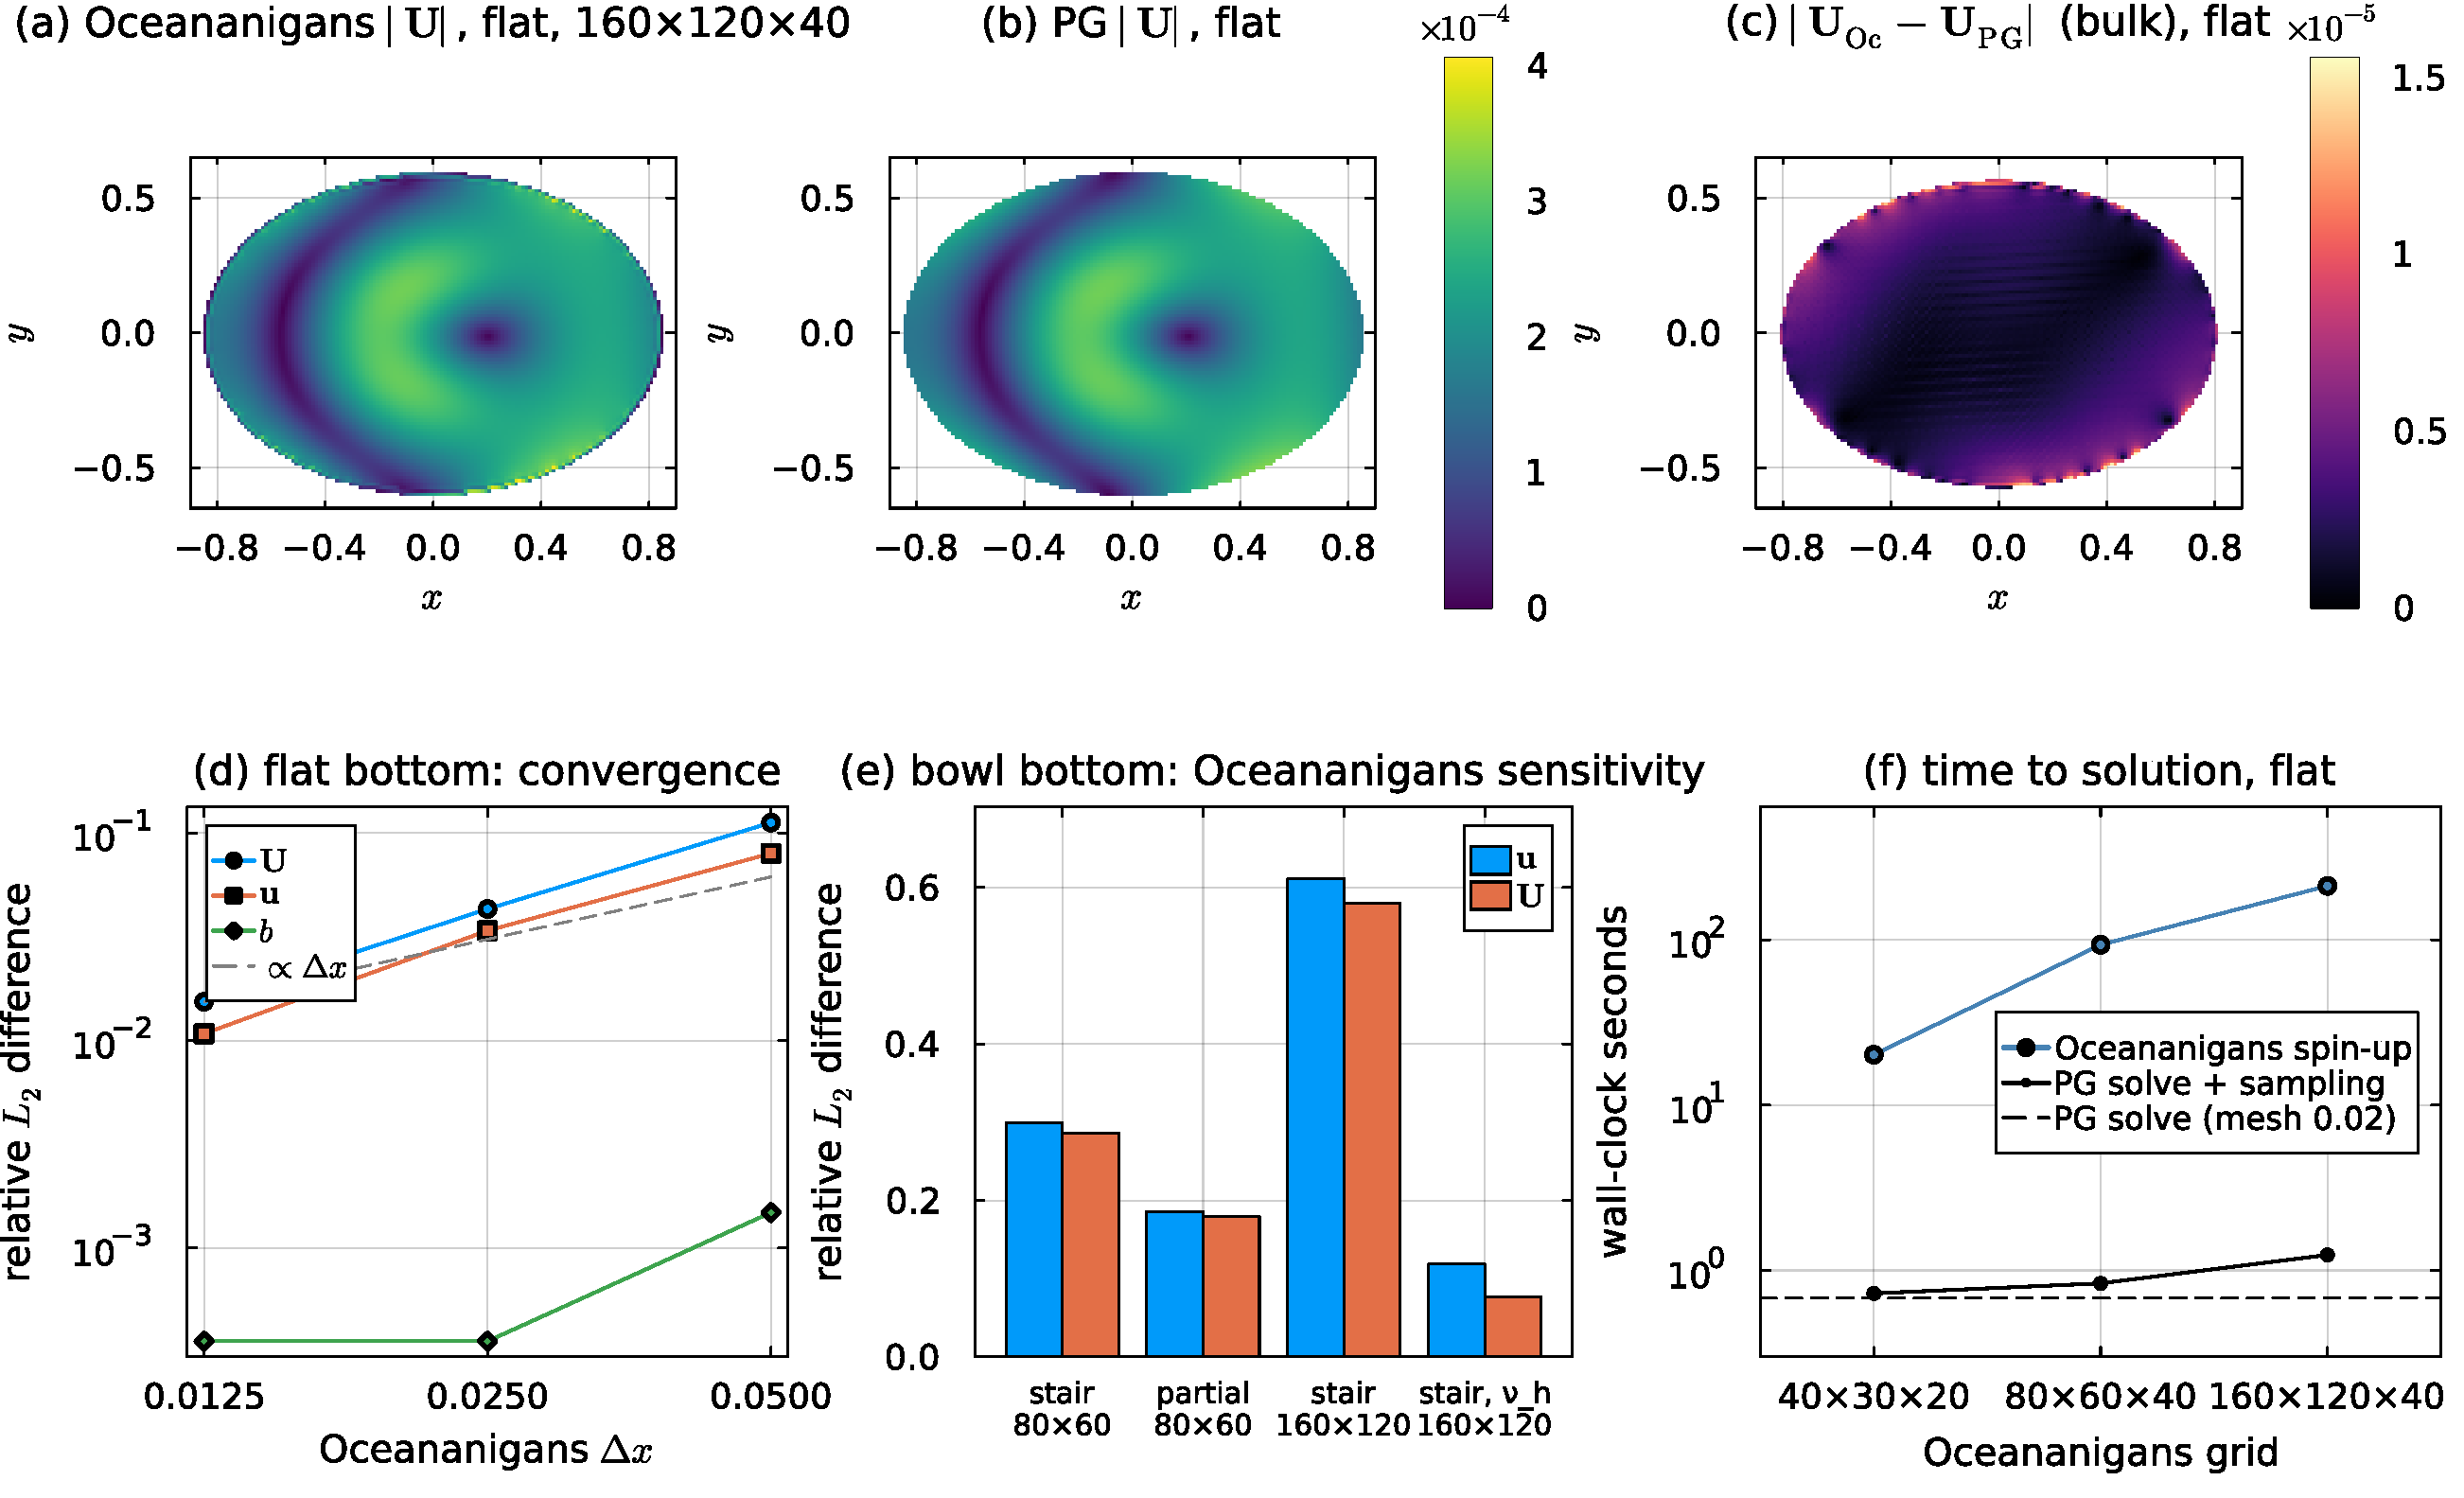
\includegraphics[width=16cm]{oceananigans_comparison.pdf}
\caption{\added[id=CL]{\label{fig:oceananigans_comparison} Comparison with \texttt{Oceananigans.jl}.
(a) \texttt{Oceananigans.jl} and (b) PG depth-integrated transport magnitude $|\mathbf{U}|$ for the flat-bottom basin on the $160 \times 120 \times 40$ grid, and (c) their difference over the comparison columns.
(d) Relative $L_2$ differences for the flat bottom against the \texttt{Oceananigans.jl} grid spacing; the gray line is proportional to $\Delta x$.
(e) Relative $L_2$ differences in $\mathbf{u}$ and $\mathbf{U}$ for the Gaussian-bowl bottom with stair-stepped and partial bottom cells, and with a horizontal viscosity $\nu_h = 10^{-4}$.
(f) Wall-clock time to solution for the flat bottom.}}
\end{figure}

\bibliographystyle{ametsoc2014}
\bibliography{references}

\end{document}